% !TeX program = xelatex
% 以本目录为工作目录，连续运行两次 xelatex main.tex。
% 不直接用 fontset=fandol 类选项：ctex 在载入文档类时套用字体集，此时 xeCJK 的默认
% 字体特性 Script=CJK 尚未清掉，会在日志里产生 fontspec 的无害警告。改为以
% fontset=none 载入，在导言区清空默认特性后再套用同一套 fandol 字体集；字体、标点
% 映射与排版结果不变（逐页渲染比对一致），日志无警告。
\documentclass[UTF8,fontset=none,a4paper,zihao=-4]{ctexart}
\defaultCJKfontfeatures{}
\ctexset{fontset=fandol}
\usepackage[margin=2.5cm]{geometry}
\usepackage{amsmath,amssymb,booktabs,longtable,array,graphicx,float}
\usepackage[section]{placeins}
\usepackage{enumitem,caption,subcaption,fancyhdr,xcolor,listings,tikz,hyperref,etoolbox}
\usetikzlibrary{arrows.meta,positioning,shapes.geometric}
\hypersetup{hidelinks,unicode=true,pdftitle={基于线性规划与滚动优化的微网电力调控策略}}
\ctexset{section={format=\centering\bfseries\large,name={,、},aftername={},number=\chinese{section},beforeskip=10pt,afterskip=5pt},subsection={format=\bfseries\normalsize,name={,\hspace{0.5em}},aftername={},beforeskip=6pt,afterskip=3pt},subsubsection={format=\bfseries\normalsize,name={,\hspace{0.5em}},aftername={},beforeskip=4pt,afterskip=2pt}}
\renewcommand{\thesubsection}{\arabic{section}.\arabic{subsection}}
\renewcommand{\thesubsubsection}{\arabic{section}.\arabic{subsection}.\arabic{subsubsection}}
\setcounter{secnumdepth}{3}
\linespread{1.10}
\setlength{\parskip}{0pt}
\setcounter{topnumber}{3}\setcounter{bottomnumber}{2}\setcounter{totalnumber}{4}
\renewcommand{\topfraction}{.88}\renewcommand{\bottomfraction}{.8}\renewcommand{\textfraction}{.1}\renewcommand{\floatpagefraction}{.8}
\setlength{\emergencystretch}{1.5em}
\clubpenalty=10000\widowpenalty=10000\displaywidowpenalty=10000
\patchcmd{\thebibliography}{\section*{\refname}}{}{}{\PackageError{main}{thebibliography heading patch failed}{}}
\setlist{nosep,leftmargin=2em}
\captionsetup{font={small,bf},labelsep=quad,skip=4pt}
\setlength{\textfloatsep}{4pt}
\setlength{\intextsep}{4pt}
\pagestyle{fancy}\fancyhf{}\fancyfoot[C]{\thepage}\renewcommand{\headrulewidth}{0pt}
\newcommand{\pos}[1]{\left[#1\right]_+}
\newcommand{\dd}{\Delta t}
\newcommand{\Emin}{E_{\min}}
\newcommand{\Emax}{E_{\max}}
\newcommand{\unit}[1]{\,\mathrm{#1}}
\lstset{language=Python,basicstyle=\ttfamily\fontsize{8.2}{10}\selectfont,commentstyle=\color{black!65},keywordstyle=\bfseries,showstringspaces=false,breaklines=true,breakatwhitespace=false,columns=fullflexible,keepspaces=true,numbers=left,numberstyle=\tiny\color{gray},numbersep=5pt,frame=single,rulecolor=\color{black!20},tabsize=4,xleftmargin=1.5em,framexleftmargin=1em}
\makeatletter\renewcommand{\@endparenv}{}\makeatother% 居中/列表环境后的段落仍保留首行缩进
\newcommand{\rv}[2]{\csname result#1#2\endcsname}
% Automatically generated; do not edit numerical values by hand.
\expandafter\def\csname resultq2kind\endcsname{2}
\expandafter\def\csname resultq2history_days\endcsname{14}
\expandafter\def\csname resultq2eta\endcsname{0.90}
\expandafter\def\csname resultq2seconds\endcsname{6.43}
\expandafter\def\csname resultq2lp_seconds\endcsname{6.32}
\expandafter\def\csname resultq2solves\endcsname{365}
\expandafter\def\csname resultq2max_eq_residual\endcsname{0.00}
\expandafter\def\csname resultq2max_ub_violation\endcsname{0.00}
\expandafter\def\csname resultq2plan_cost\endcsname{13376186.67}
\expandafter\def\csname resultq2up_cost\endcsname{0.00}
\expandafter\def\csname resultq2down_cost\endcsname{0.00}
\expandafter\def\csname resultq2emergency_cost\endcsname{487678.99}
\expandafter\def\csname resultq2total_cost\endcsname{13863865.66}
\expandafter\def\csname resultq2plan_kwh\endcsname{21791003.35}
\expandafter\def\csname resultq2grid_kwh\endcsname{21791003.35}
\expandafter\def\csname resultq2ch_kwh\endcsname{6267428.92}
\expandafter\def\csname resultq2dis_kwh\endcsname{5083626.76}
\expandafter\def\csname resultq2emergency_kwh\endcsname{85480.79}
\expandafter\def\csname resultq2spill_kwh\endcsname{2753492.48}
\expandafter\def\csname resultq2emergency_periods\endcsname{733}
\expandafter\def\csname resultq2emergency_days\endcsname{105}
\expandafter\def\csname resultq2start_energy\endcsname{9340.95}
\expandafter\def\csname resultq2end_energy\endcsname{1552.80}
\expandafter\def\csname resultq2up_kwh\endcsname{0.00}
\expandafter\def\csname resultq2down_kwh\endcsname{0.00}
\expandafter\def\csname resultq2equivalent_cycles\endcsname{587.98}
\expandafter\def\csname resultq2_nominalkind\endcsname{2}
\expandafter\def\csname resultq2_nominalhistory_days\endcsname{0}
\expandafter\def\csname resultq2_nominaleta\endcsname{0.90}
\expandafter\def\csname resultq2_nominalseconds\endcsname{1.65}
\expandafter\def\csname resultq2_nominallp_seconds\endcsname{1.58}
\expandafter\def\csname resultq2_nominalsolves\endcsname{365}
\expandafter\def\csname resultq2_nominalmax_eq_residual\endcsname{0.00}
\expandafter\def\csname resultq2_nominalmax_ub_violation\endcsname{0.00}
\expandafter\def\csname resultq2_nominalplan_cost\endcsname{12156938.16}
\expandafter\def\csname resultq2_nominalup_cost\endcsname{0.00}
\expandafter\def\csname resultq2_nominaldown_cost\endcsname{0.00}
\expandafter\def\csname resultq2_nominalemergency_cost\endcsname{3841536.66}
\expandafter\def\csname resultq2_nominaltotal_cost\endcsname{15998474.83}
\expandafter\def\csname resultq2_nominalplan_kwh\endcsname{19997187.20}
\expandafter\def\csname resultq2_nominalgrid_kwh\endcsname{19997187.20}
\expandafter\def\csname resultq2_nominalch_kwh\endcsname{6308038.25}
\expandafter\def\csname resultq2_nominaldis_kwh\endcsname{5115912.02}
\expandafter\def\csname resultq2_nominalemergency_kwh\endcsname{674346.09}
\expandafter\def\csname resultq2_nominalspill_kwh\endcsname{1540217.55}
\expandafter\def\csname resultq2_nominalemergency_periods\endcsname{4289}
\expandafter\def\csname resultq2_nominalemergency_days\endcsname{272}
\expandafter\def\csname resultq2_nominalstart_energy\endcsname{8347.72}
\expandafter\def\csname resultq2_nominalend_energy\endcsname{1235.46}
\expandafter\def\csname resultq2_nominalup_kwh\endcsname{0.00}
\expandafter\def\csname resultq2_nominaldown_kwh\endcsname{0.00}
\expandafter\def\csname resultq2_nominalequivalent_cycles\endcsname{591.75}
\expandafter\def\csname resultq3kind\endcsname{3}
\expandafter\def\csname resultq3history_days\endcsname{14}
\expandafter\def\csname resultq3eta\endcsname{0.90}
\expandafter\def\csname resultq3seconds\endcsname{17.46}
\expandafter\def\csname resultq3lp_seconds\endcsname{17.24}
\expandafter\def\csname resultq3solves\endcsname{1460}
\expandafter\def\csname resultq3max_eq_residual\endcsname{0.00}
\expandafter\def\csname resultq3max_ub_violation\endcsname{0.00}
\expandafter\def\csname resultq3plan_cost\endcsname{13564413.80}
\expandafter\def\csname resultq3up_cost\endcsname{164969.36}
\expandafter\def\csname resultq3down_cost\endcsname{-310478.47}
\expandafter\def\csname resultq3emergency_cost\endcsname{223957.35}
\expandafter\def\csname resultq3total_cost\endcsname{13642862.05}
\expandafter\def\csname resultq3plan_kwh\endcsname{22038277.07}
\expandafter\def\csname resultq3grid_kwh\endcsname{21172264.04}
\expandafter\def\csname resultq3ch_kwh\endcsname{6327180.88}
\expandafter\def\csname resultq3dis_kwh\endcsname{5132025.85}
\expandafter\def\csname resultq3emergency_kwh\endcsname{43270.28}
\expandafter\def\csname resultq3spill_kwh\endcsname{2081189.79}
\expandafter\def\csname resultq3emergency_periods\endcsname{612}
\expandafter\def\csname resultq3emergency_days\endcsname{96}
\expandafter\def\csname resultq3start_energy\endcsname{9340.95}
\expandafter\def\csname resultq3end_energy\endcsname{1552.80}
\expandafter\def\csname resultq3up_kwh\endcsname{156271.76}
\expandafter\def\csname resultq3down_kwh\endcsname{1022284.79}
\expandafter\def\csname resultq3equivalent_cycles\endcsname{593.58}
\expandafter\def\csname resultq3_dailykind\endcsname{3}
\expandafter\def\csname resultq3_dailyhistory_days\endcsname{14}
\expandafter\def\csname resultq3_dailyeta\endcsname{0.90}
\expandafter\def\csname resultq3_dailyseconds\endcsname{6.37}
\expandafter\def\csname resultq3_dailylp_seconds\endcsname{6.27}
\expandafter\def\csname resultq3_dailysolves\endcsname{365}
\expandafter\def\csname resultq3_dailymax_eq_residual\endcsname{0.00}
\expandafter\def\csname resultq3_dailymax_ub_violation\endcsname{0.00}
\expandafter\def\csname resultq3_dailyplan_cost\endcsname{13568930.46}
\expandafter\def\csname resultq3_dailyup_cost\endcsname{0.00}
\expandafter\def\csname resultq3_dailydown_cost\endcsname{0.00}
\expandafter\def\csname resultq3_dailyemergency_cost\endcsname{441424.54}
\expandafter\def\csname resultq3_dailytotal_cost\endcsname{14010355.00}
\expandafter\def\csname resultq3_dailyplan_kwh\endcsname{22048691.87}
\expandafter\def\csname resultq3_dailygrid_kwh\endcsname{22048691.87}
\expandafter\def\csname resultq3_dailych_kwh\endcsname{6240290.53}
\expandafter\def\csname resultq3_dailydis_kwh\endcsname{5061644.66}
\expandafter\def\csname resultq3_dailyemergency_kwh\endcsname{77341.11}
\expandafter\def\csname resultq3_dailyspill_kwh\endcsname{3008197.62}
\expandafter\def\csname resultq3_dailyemergency_periods\endcsname{729}
\expandafter\def\csname resultq3_dailyemergency_days\endcsname{118}
\expandafter\def\csname resultq3_dailystart_energy\endcsname{9340.95}
\expandafter\def\csname resultq3_dailyend_energy\endcsname{1552.80}
\expandafter\def\csname resultq3_dailyup_kwh\endcsname{0.00}
\expandafter\def\csname resultq3_dailydown_kwh\endcsname{0.00}
\expandafter\def\csname resultq3_dailyequivalent_cycles\endcsname{585.43}
\expandafter\def\csname resultq3_noonkind\endcsname{3}
\expandafter\def\csname resultq3_noonhistory_days\endcsname{14}
\expandafter\def\csname resultq3_nooneta\endcsname{0.90}
\expandafter\def\csname resultq3_noonseconds\endcsname{9.08}
\expandafter\def\csname resultq3_noonlp_seconds\endcsname{8.94}
\expandafter\def\csname resultq3_noonsolves\endcsname{730}
\expandafter\def\csname resultq3_noonmax_eq_residual\endcsname{0.00}
\expandafter\def\csname resultq3_noonmax_ub_violation\endcsname{0.00}
\expandafter\def\csname resultq3_noonplan_cost\endcsname{13564838.97}
\expandafter\def\csname resultq3_noonup_cost\endcsname{90237.60}
\expandafter\def\csname resultq3_noondown_cost\endcsname{-240050.46}
\expandafter\def\csname resultq3_noonemergency_cost\endcsname{324462.08}
\expandafter\def\csname resultq3_noontotal_cost\endcsname{13739488.19}
\expandafter\def\csname resultq3_noonplan_kwh\endcsname{22039263.65}
\expandafter\def\csname resultq3_noongrid_kwh\endcsname{21311018.70}
\expandafter\def\csname resultq3_noonch_kwh\endcsname{6253241.14}
\expandafter\def\csname resultq3_noondis_kwh\endcsname{5072134.66}
\expandafter\def\csname resultq3_noonemergency_kwh\endcsname{60126.17}
\expandafter\def\csname resultq3_noonspill_kwh\endcsname{2250848.89}
\expandafter\def\csname resultq3_noonemergency_periods\endcsname{677}
\expandafter\def\csname resultq3_noonemergency_days\endcsname{104}
\expandafter\def\csname resultq3_noonstart_energy\endcsname{9340.95}
\expandafter\def\csname resultq3_noonend_energy\endcsname{1552.80}
\expandafter\def\csname resultq3_noonup_kwh\endcsname{84330.60}
\expandafter\def\csname resultq3_noondown_kwh\endcsname{812575.56}
\expandafter\def\csname resultq3_noonequivalent_cycles\endcsname{586.65}
\expandafter\def\csname resultq3_additivekind\endcsname{3}
\expandafter\def\csname resultq3_additivehistory_days\endcsname{14}
\expandafter\def\csname resultq3_additiveeta\endcsname{0.90}
\expandafter\def\csname resultq3_additiveseconds\endcsname{14.97}
\expandafter\def\csname resultq3_additivelp_seconds\endcsname{14.78}
\expandafter\def\csname resultq3_additivesolves\endcsname{1460}
\expandafter\def\csname resultq3_additivemax_eq_residual\endcsname{0.00}
\expandafter\def\csname resultq3_additivemax_ub_violation\endcsname{0.00}
\expandafter\def\csname resultq3_additiveplan_cost\endcsname{13564340.98}
\expandafter\def\csname resultq3_additiveup_cost\endcsname{159758.44}
\expandafter\def\csname resultq3_additivedown_cost\endcsname{0.00}
\expandafter\def\csname resultq3_additiveemergency_cost\endcsname{210396.16}
\expandafter\def\csname resultq3_additivetotal_cost\endcsname{13934495.57}
\expandafter\def\csname resultq3_additiveplan_kwh\endcsname{22038108.09}
\expandafter\def\csname resultq3_additivegrid_kwh\endcsname{22191681.77}
\expandafter\def\csname resultq3_additivech_kwh\endcsname{6224826.76}
\expandafter\def\csname resultq3_additivedis_kwh\endcsname{5049119.01}
\expandafter\def\csname resultq3_additiveemergency_kwh\endcsname{41147.37}
\expandafter\def\csname resultq3_additivespill_kwh\endcsname{3117931.89}
\expandafter\def\csname resultq3_additiveemergency_periods\endcsname{610}
\expandafter\def\csname resultq3_additiveemergency_days\endcsname{96}
\expandafter\def\csname resultq3_additivestart_energy\endcsname{9340.95}
\expandafter\def\csname resultq3_additiveend_energy\endcsname{1552.80}
\expandafter\def\csname resultq3_additiveup_kwh\endcsname{153573.67}
\expandafter\def\csname resultq3_additivedown_kwh\endcsname{0.00}
\expandafter\def\csname resultq3_additiveequivalent_cycles\endcsname{583.98}
\expandafter\def\csname resultq4_2kind\endcsname{2}
\expandafter\def\csname resultq4_2history_days\endcsname{14}
\expandafter\def\csname resultq4_2eta\endcsname{0.90}
\expandafter\def\csname resultq4_2seconds\endcsname{5.55}
\expandafter\def\csname resultq4_2lp_seconds\endcsname{5.46}
\expandafter\def\csname resultq4_2solves\endcsname{365}
\expandafter\def\csname resultq4_2max_eq_residual\endcsname{0.00}
\expandafter\def\csname resultq4_2max_ub_violation\endcsname{0.00}
\expandafter\def\csname resultq4_2plan_cost\endcsname{14108637.49}
\expandafter\def\csname resultq4_2up_cost\endcsname{0.00}
\expandafter\def\csname resultq4_2down_cost\endcsname{0.00}
\expandafter\def\csname resultq4_2emergency_cost\endcsname{512777.68}
\expandafter\def\csname resultq4_2total_cost\endcsname{14621415.17}
\expandafter\def\csname resultq4_2plan_kwh\endcsname{21789163.61}
\expandafter\def\csname resultq4_2grid_kwh\endcsname{21789163.61}
\expandafter\def\csname resultq4_2ch_kwh\endcsname{6304696.37}
\expandafter\def\csname resultq4_2dis_kwh\endcsname{5113706.46}
\expandafter\def\csname resultq4_2emergency_kwh\endcsname{83563.75}
\expandafter\def\csname resultq4_2spill_kwh\endcsname{2742547.96}
\expandafter\def\csname resultq4_2emergency_periods\endcsname{731}
\expandafter\def\csname resultq4_2emergency_days\endcsname{101}
\expandafter\def\csname resultq4_2start_energy\endcsname{9218.19}
\expandafter\def\csname resultq4_2end_energy\endcsname{1548.85}
\expandafter\def\csname resultq4_2up_kwh\endcsname{0.00}
\expandafter\def\csname resultq4_2down_kwh\endcsname{0.00}
\expandafter\def\csname resultq4_2equivalent_cycles\endcsname{591.46}
\expandafter\def\csname resultq4_3kind\endcsname{3}
\expandafter\def\csname resultq4_3history_days\endcsname{14}
\expandafter\def\csname resultq4_3eta\endcsname{0.90}
\expandafter\def\csname resultq4_3seconds\endcsname{17.09}
\expandafter\def\csname resultq4_3lp_seconds\endcsname{16.87}
\expandafter\def\csname resultq4_3solves\endcsname{1460}
\expandafter\def\csname resultq4_3max_eq_residual\endcsname{0.00}
\expandafter\def\csname resultq4_3max_ub_violation\endcsname{0.00}
\expandafter\def\csname resultq4_3plan_cost\endcsname{14313292.55}
\expandafter\def\csname resultq4_3up_cost\endcsname{178114.40}
\expandafter\def\csname resultq4_3down_cost\endcsname{-330099.56}
\expandafter\def\csname resultq4_3emergency_cost\endcsname{242365.43}
\expandafter\def\csname resultq4_3total_cost\endcsname{14403672.82}
\expandafter\def\csname resultq4_3plan_kwh\endcsname{22043028.66}
\expandafter\def\csname resultq4_3grid_kwh\endcsname{21159936.53}
\expandafter\def\csname resultq4_3ch_kwh\endcsname{6367230.34}
\expandafter\def\csname resultq4_3dis_kwh\endcsname{5164358.98}
\expandafter\def\csname resultq4_3emergency_kwh\endcsname{43101.90}
\expandafter\def\csname resultq4_3spill_kwh\endcsname{2060977.57}
\expandafter\def\csname resultq4_3emergency_periods\endcsname{628}
\expandafter\def\csname resultq4_3emergency_days\endcsname{93}
\expandafter\def\csname resultq4_3start_energy\endcsname{9218.19}
\expandafter\def\csname resultq4_3end_energy\endcsname{1548.85}
\expandafter\def\csname resultq4_3up_kwh\endcsname{154102.64}
\expandafter\def\csname resultq4_3down_kwh\endcsname{1037194.76}
\expandafter\def\csname resultq4_3equivalent_cycles\endcsname{597.33}
\expandafter\def\csname resultq4_2_knownkind\endcsname{2}
\expandafter\def\csname resultq4_2_knownhistory_days\endcsname{14}
\expandafter\def\csname resultq4_2_knowneta\endcsname{0.90}
\expandafter\def\csname resultq4_2_knownseconds\endcsname{6.54}
\expandafter\def\csname resultq4_2_knownlp_seconds\endcsname{6.42}
\expandafter\def\csname resultq4_2_knownsolves\endcsname{365}
\expandafter\def\csname resultq4_2_knownmax_eq_residual\endcsname{0.00}
\expandafter\def\csname resultq4_2_knownmax_ub_violation\endcsname{0.00}
\expandafter\def\csname resultq4_2_knownplan_cost\endcsname{13983171.58}
\expandafter\def\csname resultq4_2_knownup_cost\endcsname{0.00}
\expandafter\def\csname resultq4_2_knowndown_cost\endcsname{0.00}
\expandafter\def\csname resultq4_2_knownemergency_cost\endcsname{533673.99}
\expandafter\def\csname resultq4_2_knowntotal_cost\endcsname{14516845.57}
\expandafter\def\csname resultq4_2_knownplan_kwh\endcsname{21848421.32}
\expandafter\def\csname resultq4_2_knowngrid_kwh\endcsname{21848421.32}
\expandafter\def\csname resultq4_2_knownch_kwh\endcsname{6631563.84}
\expandafter\def\csname resultq4_2_knowndis_kwh\endcsname{5378359.89}
\expandafter\def\csname resultq4_2_knownemergency_kwh\endcsname{86659.63}
\expandafter\def\csname resultq4_2_knownspill_kwh\endcsname{2742687.50}
\expandafter\def\csname resultq4_2_knownemergency_periods\endcsname{743}
\expandafter\def\csname resultq4_2_knownemergency_days\endcsname{120}
\expandafter\def\csname resultq4_2_knownstart_energy\endcsname{9080.29}
\expandafter\def\csname resultq4_2_knownend_energy\endcsname{1532.32}
\expandafter\def\csname resultq4_2_knownup_kwh\endcsname{0.00}
\expandafter\def\csname resultq4_2_knowndown_kwh\endcsname{0.00}
\expandafter\def\csname resultq4_2_knownequivalent_cycles\endcsname{622.10}
\expandafter\def\csname resultq4_3_knownkind\endcsname{3}
\expandafter\def\csname resultq4_3_knownhistory_days\endcsname{14}
\expandafter\def\csname resultq4_3_knowneta\endcsname{0.90}
\expandafter\def\csname resultq4_3_knownseconds\endcsname{15.38}
\expandafter\def\csname resultq4_3_knownlp_seconds\endcsname{15.19}
\expandafter\def\csname resultq4_3_knownsolves\endcsname{1460}
\expandafter\def\csname resultq4_3_knownmax_eq_residual\endcsname{0.00}
\expandafter\def\csname resultq4_3_knownmax_ub_violation\endcsname{0.00}
\expandafter\def\csname resultq4_3_knownplan_cost\endcsname{14183750.66}
\expandafter\def\csname resultq4_3_knownup_cost\endcsname{180082.39}
\expandafter\def\csname resultq4_3_knowndown_cost\endcsname{-323891.07}
\expandafter\def\csname resultq4_3_knownemergency_cost\endcsname{243379.58}
\expandafter\def\csname resultq4_3_knowntotal_cost\endcsname{14283321.56}
\expandafter\def\csname resultq4_3_knownplan_kwh\endcsname{22096268.63}
\expandafter\def\csname resultq4_3_knowngrid_kwh\endcsname{21237509.43}
\expandafter\def\csname resultq4_3_knownch_kwh\endcsname{6687940.81}
\expandafter\def\csname resultq4_3_knowndis_kwh\endcsname{5424025.23}
\expandafter\def\csname resultq4_3_knownemergency_kwh\endcsname{43877.11}
\expandafter\def\csname resultq4_3_knownspill_kwh\endcsname{2078281.47}
\expandafter\def\csname resultq4_3_knownemergency_periods\endcsname{647}
\expandafter\def\csname resultq4_3_knownemergency_days\endcsname{106}
\expandafter\def\csname resultq4_3_knownstart_energy\endcsname{9080.29}
\expandafter\def\csname resultq4_3_knownend_energy\endcsname{1532.32}
\expandafter\def\csname resultq4_3_knownup_kwh\endcsname{159408.46}
\expandafter\def\csname resultq4_3_knowndown_kwh\endcsname{1018167.66}
\expandafter\def\csname resultq4_3_knownequivalent_cycles\endcsname{627.39}
\expandafter\def\csname resultq4_3_additivekind\endcsname{3}
\expandafter\def\csname resultq4_3_additivehistory_days\endcsname{14}
\expandafter\def\csname resultq4_3_additiveeta\endcsname{0.90}
\expandafter\def\csname resultq4_3_additiveseconds\endcsname{14.99}
\expandafter\def\csname resultq4_3_additivelp_seconds\endcsname{14.80}
\expandafter\def\csname resultq4_3_additivesolves\endcsname{1460}
\expandafter\def\csname resultq4_3_additivemax_eq_residual\endcsname{0.00}
\expandafter\def\csname resultq4_3_additivemax_ub_violation\endcsname{0.00}
\expandafter\def\csname resultq4_3_additiveplan_cost\endcsname{14313150.95}
\expandafter\def\csname resultq4_3_additiveup_cost\endcsname{173002.22}
\expandafter\def\csname resultq4_3_additivedown_cost\endcsname{0.00}
\expandafter\def\csname resultq4_3_additiveemergency_cost\endcsname{225604.34}
\expandafter\def\csname resultq4_3_additivetotal_cost\endcsname{14711757.51}
\expandafter\def\csname resultq4_3_additiveplan_kwh\endcsname{22042699.70}
\expandafter\def\csname resultq4_3_additivegrid_kwh\endcsname{22194208.88}
\expandafter\def\csname resultq4_3_additivech_kwh\endcsname{6277993.60}
\expandafter\def\csname resultq4_3_additivedis_kwh\endcsname{5092077.22}
\expandafter\def\csname resultq4_3_additiveemergency_kwh\endcsname{40537.46}
\expandafter\def\csname resultq4_3_additivespill_kwh\endcsname{3109640.46}
\expandafter\def\csname resultq4_3_additiveemergency_periods\endcsname{622}
\expandafter\def\csname resultq4_3_additiveemergency_days\endcsname{92}
\expandafter\def\csname resultq4_3_additivestart_energy\endcsname{9218.19}
\expandafter\def\csname resultq4_3_additiveend_energy\endcsname{1548.85}
\expandafter\def\csname resultq4_3_additiveup_kwh\endcsname{151509.17}
\expandafter\def\csname resultq4_3_additivedown_kwh\endcsname{0.00}
\expandafter\def\csname resultq4_3_additiveequivalent_cycles\endcsname{588.96}
\expandafter\def\csname resultq3_history7kind\endcsname{3}
\expandafter\def\csname resultq3_history7history_days\endcsname{7}
\expandafter\def\csname resultq3_history7eta\endcsname{0.90}
\expandafter\def\csname resultq3_history7seconds\endcsname{10.55}
\expandafter\def\csname resultq3_history7lp_seconds\endcsname{10.37}
\expandafter\def\csname resultq3_history7solves\endcsname{1460}
\expandafter\def\csname resultq3_history7max_eq_residual\endcsname{0.00}
\expandafter\def\csname resultq3_history7max_ub_violation\endcsname{0.00}
\expandafter\def\csname resultq3_history7plan_cost\endcsname{13426769.89}
\expandafter\def\csname resultq3_history7up_cost\endcsname{177843.35}
\expandafter\def\csname resultq3_history7down_cost\endcsname{-276072.58}
\expandafter\def\csname resultq3_history7emergency_cost\endcsname{157987.57}
\expandafter\def\csname resultq3_history7total_cost\endcsname{13486528.22}
\expandafter\def\csname resultq3_history7plan_kwh\endcsname{21877168.47}
\expandafter\def\csname resultq3_history7grid_kwh\endcsname{21121333.37}
\expandafter\def\csname resultq3_history7ch_kwh\endcsname{6374141.97}
\expandafter\def\csname resultq3_history7dis_kwh\endcsname{5170100.13}
\expandafter\def\csname resultq3_history7emergency_kwh\endcsname{30405.57}
\expandafter\def\csname resultq3_history7spill_kwh\endcsname{2008507.61}
\expandafter\def\csname resultq3_history7emergency_periods\endcsname{453}
\expandafter\def\csname resultq3_history7emergency_days\endcsname{103}
\expandafter\def\csname resultq3_history7start_energy\endcsname{9175.29}
\expandafter\def\csname resultq3_history7end_energy\endcsname{1347.37}
\expandafter\def\csname resultq3_history7up_kwh\endcsname{167946.00}
\expandafter\def\csname resultq3_history7down_kwh\endcsname{923781.11}
\expandafter\def\csname resultq3_history7equivalent_cycles\endcsname{597.98}
\expandafter\def\csname resultq3_history28kind\endcsname{3}
\expandafter\def\csname resultq3_history28history_days\endcsname{28}
\expandafter\def\csname resultq3_history28eta\endcsname{0.90}
\expandafter\def\csname resultq3_history28seconds\endcsname{27.57}
\expandafter\def\csname resultq3_history28lp_seconds\endcsname{27.32}
\expandafter\def\csname resultq3_history28solves\endcsname{1460}
\expandafter\def\csname resultq3_history28max_eq_residual\endcsname{0.00}
\expandafter\def\csname resultq3_history28max_ub_violation\endcsname{0.00}
\expandafter\def\csname resultq3_history28plan_cost\endcsname{13599098.44}
\expandafter\def\csname resultq3_history28up_cost\endcsname{166926.76}
\expandafter\def\csname resultq3_history28down_cost\endcsname{-281351.53}
\expandafter\def\csname resultq3_history28emergency_cost\endcsname{253280.53}
\expandafter\def\csname resultq3_history28total_cost\endcsname{13737954.20}
\expandafter\def\csname resultq3_history28plan_kwh\endcsname{22076626.34}
\expandafter\def\csname resultq3_history28grid_kwh\endcsname{21288550.71}
\expandafter\def\csname resultq3_history28ch_kwh\endcsname{6301690.99}
\expandafter\def\csname resultq3_history28dis_kwh\endcsname{5111287.24}
\expandafter\def\csname resultq3_history28emergency_kwh\endcsname{49801.19}
\expandafter\def\csname resultq3_history28spill_kwh\endcsname{2208758.66}
\expandafter\def\csname resultq3_history28emergency_periods\endcsname{747}
\expandafter\def\csname resultq3_history28emergency_days\endcsname{101}
\expandafter\def\csname resultq3_history28start_energy\endcsname{9353.45}
\expandafter\def\csname resultq3_history28end_energy\endcsname{1667.29}
\expandafter\def\csname resultq3_history28up_kwh\endcsname{158747.50}
\expandafter\def\csname resultq3_history28down_kwh\endcsname{946823.13}
\expandafter\def\csname resultq3_history28equivalent_cycles\endcsname{591.18}
\expandafter\def\csname resultq3_blendkind\endcsname{3}
\expandafter\def\csname resultq3_blendhistory_days\endcsname{14}
\expandafter\def\csname resultq3_blendeta\endcsname{0.90}
\expandafter\def\csname resultq3_blendseconds\endcsname{16.74}
\expandafter\def\csname resultq3_blendlp_seconds\endcsname{16.49}
\expandafter\def\csname resultq3_blendsolves\endcsname{1460}
\expandafter\def\csname resultq3_blendmax_eq_residual\endcsname{0.00}
\expandafter\def\csname resultq3_blendmax_ub_violation\endcsname{0.00}
\expandafter\def\csname resultq3_blendplan_cost\endcsname{13292333.82}
\expandafter\def\csname resultq3_blendup_cost\endcsname{76437.83}
\expandafter\def\csname resultq3_blenddown_cost\endcsname{-145294.15}
\expandafter\def\csname resultq3_blendemergency_cost\endcsname{238269.27}
\expandafter\def\csname resultq3_blendtotal_cost\endcsname{13461746.78}
\expandafter\def\csname resultq3_blendplan_kwh\endcsname{21649494.23}
\expandafter\def\csname resultq3_blendgrid_kwh\endcsname{21176122.86}
\expandafter\def\csname resultq3_blendch_kwh\endcsname{6325611.90}
\expandafter\def\csname resultq3_blenddis_kwh\endcsname{5130754.98}
\expandafter\def\csname resultq3_blendemergency_kwh\endcsname{46172.34}
\expandafter\def\csname resultq3_blendspill_kwh\endcsname{2088248.78}
\expandafter\def\csname resultq3_blendemergency_periods\endcsname{638}
\expandafter\def\csname resultq3_blendemergency_days\endcsname{96}
\expandafter\def\csname resultq3_blendstart_energy\endcsname{9340.95}
\expandafter\def\csname resultq3_blendend_energy\endcsname{1552.80}
\expandafter\def\csname resultq3_blendup_kwh\endcsname{62442.55}
\expandafter\def\csname resultq3_blenddown_kwh\endcsname{535813.92}
\expandafter\def\csname resultq3_blendequivalent_cycles\endcsname{593.43}
\expandafter\def\csname resultq4_3_blendkind\endcsname{3}
\expandafter\def\csname resultq4_3_blendhistory_days\endcsname{14}
\expandafter\def\csname resultq4_3_blendeta\endcsname{0.90}
\expandafter\def\csname resultq4_3_blendseconds\endcsname{16.28}
\expandafter\def\csname resultq4_3_blendlp_seconds\endcsname{16.06}
\expandafter\def\csname resultq4_3_blendsolves\endcsname{1460}
\expandafter\def\csname resultq4_3_blendmax_eq_residual\endcsname{0.00}
\expandafter\def\csname resultq4_3_blendmax_ub_violation\endcsname{0.00}
\expandafter\def\csname resultq4_3_blendplan_cost\endcsname{14024694.81}
\expandafter\def\csname resultq4_3_blendup_cost\endcsname{83684.26}
\expandafter\def\csname resultq4_3_blenddown_cost\endcsname{-151450.13}
\expandafter\def\csname resultq4_3_blendemergency_cost\endcsname{250556.40}
\expandafter\def\csname resultq4_3_blendtotal_cost\endcsname{14207485.34}
\expandafter\def\csname resultq4_3_blendplan_kwh\endcsname{21650475.10}
\expandafter\def\csname resultq4_3_blendgrid_kwh\endcsname{21183710.28}
\expandafter\def\csname resultq4_3_blendch_kwh\endcsname{6365812.03}
\expandafter\def\csname resultq4_3_blenddis_kwh\endcsname{5163210.15}
\expandafter\def\csname resultq4_3_blendemergency_kwh\endcsname{44752.90}
\expandafter\def\csname resultq4_3_blendspill_kwh\endcsname{2086671.80}
\expandafter\def\csname resultq4_3_blendemergency_periods\endcsname{646}
\expandafter\def\csname resultq4_3_blendemergency_days\endcsname{92}
\expandafter\def\csname resultq4_3_blendstart_energy\endcsname{9218.19}
\expandafter\def\csname resultq4_3_blendend_energy\endcsname{1548.85}
\expandafter\def\csname resultq4_3_blendup_kwh\endcsname{62523.70}
\expandafter\def\csname resultq4_3_blenddown_kwh\endcsname{529288.52}
\expandafter\def\csname resultq4_3_blendequivalent_cycles\endcsname{597.19}
\expandafter\def\csname resultq3d0320plan\endcsname{71993.11}
\expandafter\def\csname resultq3d0320grid\endcsname{66853.81}
\expandafter\def\csname resultq3d0320emergency\endcsname{113.04}
\expandafter\def\csname resultq3d0320total\endcsname{43037.70}
\expandafter\def\csname resultq3d0320up_cost\endcsname{14.64}
\expandafter\def\csname resultq3d0320down_cost\endcsname{-1771.73}
\expandafter\def\csname resultq3d0320up\endcsname{13.38}
\expandafter\def\csname resultq3d0320down\endcsname{5152.68}
\expandafter\def\csname resultq3d0621plan\endcsname{35054.77}
\expandafter\def\csname resultq3d0621grid\endcsname{34929.74}
\expandafter\def\csname resultq3d0621emergency\endcsname{0.00}
\expandafter\def\csname resultq3d0621total\endcsname{20690.52}
\expandafter\def\csname resultq3d0621up_cost\endcsname{0.00}
\expandafter\def\csname resultq3d0621down_cost\endcsname{-52.61}
\expandafter\def\csname resultq3d0621up\endcsname{0.00}
\expandafter\def\csname resultq3d0621down\endcsname{125.03}
\expandafter\def\csname resultq3d0923plan\endcsname{72432.47}
\expandafter\def\csname resultq3d0923grid\endcsname{67541.88}
\expandafter\def\csname resultq3d0923emergency\endcsname{464.02}
\expandafter\def\csname resultq3d0923total\endcsname{46227.25}
\expandafter\def\csname resultq3d0923up_cost\endcsname{0.00}
\expandafter\def\csname resultq3d0923down_cost\endcsname{-1414.81}
\expandafter\def\csname resultq3d0923up\endcsname{0.00}
\expandafter\def\csname resultq3d0923down\endcsname{4890.59}
\expandafter\def\csname resultq3d1221plan\endcsname{99503.29}
\expandafter\def\csname resultq3d1221grid\endcsname{97280.92}
\expandafter\def\csname resultq3d1221emergency\endcsname{0.00}
\expandafter\def\csname resultq3d1221total\endcsname{63388.89}
\expandafter\def\csname resultq3d1221up_cost\endcsname{0.00}
\expandafter\def\csname resultq3d1221down_cost\endcsname{-696.53}
\expandafter\def\csname resultq3d1221up\endcsname{0.00}
\expandafter\def\csname resultq3d1221down\endcsname{2222.37}
\expandafter\def\csname resultq4_3d0320plan\endcsname{71871.84}
\expandafter\def\csname resultq4_3d0320grid\endcsname{66695.93}
\expandafter\def\csname resultq4_3d0320emergency\endcsname{114.06}
\expandafter\def\csname resultq4_3d0320total\endcsname{44535.29}
\expandafter\def\csname resultq4_3d0320up_cost\endcsname{21.02}
\expandafter\def\csname resultq4_3d0320down_cost\endcsname{-1911.07}
\expandafter\def\csname resultq4_3d0320up\endcsname{18.28}
\expandafter\def\csname resultq4_3d0320down\endcsname{5194.20}
\expandafter\def\csname resultq4_3d0621plan\endcsname{35397.64}
\expandafter\def\csname resultq4_3d0621grid\endcsname{35241.80}
\expandafter\def\csname resultq4_3d0621emergency\endcsname{0.00}
\expandafter\def\csname resultq4_3d0621total\endcsname{18088.21}
\expandafter\def\csname resultq4_3d0621up_cost\endcsname{0.00}
\expandafter\def\csname resultq4_3d0621down_cost\endcsname{-45.83}
\expandafter\def\csname resultq4_3d0621up\endcsname{0.00}
\expandafter\def\csname resultq4_3d0621down\endcsname{155.84}
\expandafter\def\csname resultq4_3d0923plan\endcsname{72586.44}
\expandafter\def\csname resultq4_3d0923grid\endcsname{67662.34}
\expandafter\def\csname resultq4_3d0923emergency\endcsname{466.14}
\expandafter\def\csname resultq4_3d0923total\endcsname{48346.91}
\expandafter\def\csname resultq4_3d0923up_cost\endcsname{0.00}
\expandafter\def\csname resultq4_3d0923down_cost\endcsname{-1375.50}
\expandafter\def\csname resultq4_3d0923up\endcsname{0.00}
\expandafter\def\csname resultq4_3d0923down\endcsname{4924.10}
\expandafter\def\csname resultq4_3d1221plan\endcsname{99343.17}
\expandafter\def\csname resultq4_3d1221grid\endcsname{97208.96}
\expandafter\def\csname resultq4_3d1221emergency\endcsname{0.00}
\expandafter\def\csname resultq4_3d1221total\endcsname{74630.49}
\expandafter\def\csname resultq4_3d1221up_cost\endcsname{0.00}
\expandafter\def\csname resultq4_3d1221down_cost\endcsname{-996.47}
\expandafter\def\csname resultq4_3d1221up\endcsname{0.00}
\expandafter\def\csname resultq4_3d1221down\endcsname{2134.21}
\expandafter\def\csname resultderivedcase_count\endcsname{15}
\expandafter\def\csname resultderivedfrequency_saving\endcsname{367492.96}
\expandafter\def\csname resultderivedfrequency_percent\endcsname{2.62}
\expandafter\def\csname resultderivednoon_saving\endcsname{96626.14}
\expandafter\def\csname resultderivednoon_percent\endcsname{0.70}
\expandafter\def\csname resultderivedq3_vs_q2_saving\endcsname{221003.61}
\expandafter\def\csname resultderivedq3_vs_q2_percent\endcsname{1.59}
\expandafter\def\csname resultderivedprice2_saving\endcsname{104569.60}
\expandafter\def\csname resultderivedprice2_percent\endcsname{0.72}
\expandafter\def\csname resultderivedprice3_saving\endcsname{120351.26}
\expandafter\def\csname resultderivedprice3_percent\endcsname{0.84}
\expandafter\def\csname resultderivedsettlement3_saving\endcsname{291633.53}
\expandafter\def\csname resultderivedsettlement3_percent\endcsname{2.09}
\expandafter\def\csname resultderivedsettlement4_saving\endcsname{308084.69}
\expandafter\def\csname resultderivedsettlement4_percent\endcsname{2.09}
\expandafter\def\csname resultderivedblend3_saving\endcsname{181115.27}
\expandafter\def\csname resultderivedblend3_percent\endcsname{1.33}
\expandafter\def\csname resultderivedblend4_saving\endcsname{196187.48}
\expandafter\def\csname resultderivedblend4_percent\endcsname{1.36}
\expandafter\def\csname resultderivedfrequency_em_percent\endcsname{44.05}
\expandafter\def\csname resultderivedcheaper\endcsname{261}
\expandafter\def\csname resultderivedmore_expensive\endcsname{67}
\expandafter\def\csname resultderivedsame\endcsname{6}

% Generated by refinement_evidence.py; no handwritten result values.
\expandafter\def\csname resultq2_terminalkind\endcsname{2}
\expandafter\def\csname resultq2_terminaleta\endcsname{0.90}
\expandafter\def\csname resultq2_terminalgamma\endcsname{0.00}
\expandafter\def\csname resultq2_terminalgate\endcsname{False}
\expandafter\def\csname resultq2_terminalstart_day\endcsname{31}
\expandafter\def\csname resultq2_terminalstop_day\endcsname{365}
\expandafter\def\csname resultq2_terminaldaily_oracle\endcsname{False}
\expandafter\def\csname resultq2_terminalseconds\endcsname{5.80}
\expandafter\def\csname resultq2_terminallp_seconds\endcsname{5.70}
\expandafter\def\csname resultq2_terminalsolves\endcsname{334}
\expandafter\def\csname resultq2_terminalaccepted\endcsname{0}
\expandafter\def\csname resultq2_terminalrejected\endcsname{0}
\expandafter\def\csname resultq2_terminalplan_cost\endcsname{13376186.67}
\expandafter\def\csname resultq2_terminalup_cost\endcsname{0.00}
\expandafter\def\csname resultq2_terminaldown_cost\endcsname{0.00}
\expandafter\def\csname resultq2_terminalemergency_cost\endcsname{487678.99}
\expandafter\def\csname resultq2_terminaltotal_cost\endcsname{13863865.66}
\expandafter\def\csname resultq2_terminalplan_kwh\endcsname{21791003.35}
\expandafter\def\csname resultq2_terminalgrid_kwh\endcsname{21791003.35}
\expandafter\def\csname resultq2_terminalch_kwh\endcsname{6267428.92}
\expandafter\def\csname resultq2_terminaldis_kwh\endcsname{5083626.76}
\expandafter\def\csname resultq2_terminalemergency_kwh\endcsname{85480.79}
\expandafter\def\csname resultq2_terminalspill_kwh\endcsname{2753492.48}
\expandafter\def\csname resultq2_terminalemergency_periods\endcsname{733}
\expandafter\def\csname resultq2_terminalemergency_days\endcsname{105}
\expandafter\def\csname resultq2_terminalstart_energy\endcsname{9340.95}
\expandafter\def\csname resultq2_terminalend_energy\endcsname{1552.80}
\expandafter\def\csname resultq2_terminalup_kwh\endcsname{0.00}
\expandafter\def\csname resultq2_terminaldown_kwh\endcsname{0.00}
\expandafter\def\csname resultq2_terminalequivalent_cycles\endcsname{587.98}
\expandafter\def\csname resultq2_economickind\endcsname{2}
\expandafter\def\csname resultq2_economiceta\endcsname{0.90}
\expandafter\def\csname resultq2_economicgamma\endcsname{0.00}
\expandafter\def\csname resultq2_economicgate\endcsname{False}
\expandafter\def\csname resultq2_economicstart_day\endcsname{31}
\expandafter\def\csname resultq2_economicstop_day\endcsname{365}
\expandafter\def\csname resultq2_economicdaily_oracle\endcsname{False}
\expandafter\def\csname resultq2_economicseconds\endcsname{5.41}
\expandafter\def\csname resultq2_economiclp_seconds\endcsname{5.33}
\expandafter\def\csname resultq2_economicsolves\endcsname{334}
\expandafter\def\csname resultq2_economicaccepted\endcsname{0}
\expandafter\def\csname resultq2_economicrejected\endcsname{0}
\expandafter\def\csname resultq2_economicplan_cost\endcsname{13406834.13}
\expandafter\def\csname resultq2_economicup_cost\endcsname{0.00}
\expandafter\def\csname resultq2_economicdown_cost\endcsname{0.00}
\expandafter\def\csname resultq2_economicemergency_cost\endcsname{451895.79}
\expandafter\def\csname resultq2_economictotal_cost\endcsname{13858729.92}
\expandafter\def\csname resultq2_economicplan_kwh\endcsname{21841056.21}
\expandafter\def\csname resultq2_economicgrid_kwh\endcsname{21841056.21}
\expandafter\def\csname resultq2_economicch_kwh\endcsname{6261401.62}
\expandafter\def\csname resultq2_economicdis_kwh\endcsname{5078744.65}
\expandafter\def\csname resultq2_economicemergency_kwh\endcsname{80511.05}
\expandafter\def\csname resultq2_economicspill_kwh\endcsname{2799720.80}
\expandafter\def\csname resultq2_economicemergency_periods\endcsname{747}
\expandafter\def\csname resultq2_economicemergency_days\endcsname{113}
\expandafter\def\csname resultq2_economicstart_energy\endcsname{9340.95}
\expandafter\def\csname resultq2_economicend_energy\endcsname{1552.80}
\expandafter\def\csname resultq2_economicup_kwh\endcsname{0.00}
\expandafter\def\csname resultq2_economicdown_kwh\endcsname{0.00}
\expandafter\def\csname resultq2_economicequivalent_cycles\endcsname{587.41}
\expandafter\def\csname resultq2_mae_controlkind\endcsname{2}
\expandafter\def\csname resultq2_mae_controleta\endcsname{0.90}
\expandafter\def\csname resultq2_mae_controlgamma\endcsname{0.00}
\expandafter\def\csname resultq2_mae_controlgate\endcsname{False}
\expandafter\def\csname resultq2_mae_controlstart_day\endcsname{31}
\expandafter\def\csname resultq2_mae_controlstop_day\endcsname{365}
\expandafter\def\csname resultq2_mae_controldaily_oracle\endcsname{False}
\expandafter\def\csname resultq2_mae_controlseconds\endcsname{5.67}
\expandafter\def\csname resultq2_mae_controllp_seconds\endcsname{5.58}
\expandafter\def\csname resultq2_mae_controlsolves\endcsname{334}
\expandafter\def\csname resultq2_mae_controlaccepted\endcsname{0}
\expandafter\def\csname resultq2_mae_controlrejected\endcsname{0}
\expandafter\def\csname resultq2_mae_controlplan_cost\endcsname{13364612.38}
\expandafter\def\csname resultq2_mae_controlup_cost\endcsname{0.00}
\expandafter\def\csname resultq2_mae_controldown_cost\endcsname{0.00}
\expandafter\def\csname resultq2_mae_controlemergency_cost\endcsname{487678.99}
\expandafter\def\csname resultq2_mae_controltotal_cost\endcsname{13852291.37}
\expandafter\def\csname resultq2_mae_controlplan_kwh\endcsname{21774732.61}
\expandafter\def\csname resultq2_mae_controlgrid_kwh\endcsname{21774732.61}
\expandafter\def\csname resultq2_mae_controlch_kwh\endcsname{6273340.83}
\expandafter\def\csname resultq2_mae_controldis_kwh\endcsname{5088415.41}
\expandafter\def\csname resultq2_mae_controlemergency_kwh\endcsname{85480.79}
\expandafter\def\csname resultq2_mae_controlspill_kwh\endcsname{2736098.48}
\expandafter\def\csname resultq2_mae_controlemergency_periods\endcsname{733}
\expandafter\def\csname resultq2_mae_controlemergency_days\endcsname{105}
\expandafter\def\csname resultq2_mae_controlstart_energy\endcsname{9340.95}
\expandafter\def\csname resultq2_mae_controlend_energy\endcsname{1552.80}
\expandafter\def\csname resultq2_mae_controlup_kwh\endcsname{0.00}
\expandafter\def\csname resultq2_mae_controldown_kwh\endcsname{0.00}
\expandafter\def\csname resultq2_mae_controlequivalent_cycles\endcsname{588.53}
\expandafter\def\csname resultq2_daily_oraclekind\endcsname{2}
\expandafter\def\csname resultq2_daily_oracleeta\endcsname{0.90}
\expandafter\def\csname resultq2_daily_oraclegamma\endcsname{0.00}
\expandafter\def\csname resultq2_daily_oraclegate\endcsname{False}
\expandafter\def\csname resultq2_daily_oraclestart_day\endcsname{31}
\expandafter\def\csname resultq2_daily_oraclestop_day\endcsname{365}
\expandafter\def\csname resultq2_daily_oracledaily_oracle\endcsname{True}
\expandafter\def\csname resultq2_daily_oracleseconds\endcsname{1.62}
\expandafter\def\csname resultq2_daily_oraclelp_seconds\endcsname{1.55}
\expandafter\def\csname resultq2_daily_oraclesolves\endcsname{334}
\expandafter\def\csname resultq2_daily_oracleaccepted\endcsname{0}
\expandafter\def\csname resultq2_daily_oraclerejected\endcsname{0}
\expandafter\def\csname resultq2_daily_oracleplan_cost\endcsname{12250938.36}
\expandafter\def\csname resultq2_daily_oracleup_cost\endcsname{0.00}
\expandafter\def\csname resultq2_daily_oracledown_cost\endcsname{0.00}
\expandafter\def\csname resultq2_daily_oracleemergency_cost\endcsname{0.00}
\expandafter\def\csname resultq2_daily_oracletotal_cost\endcsname{12250938.36}
\expandafter\def\csname resultq2_daily_oracleplan_kwh\endcsname{20180770.30}
\expandafter\def\csname resultq2_daily_oraclegrid_kwh\endcsname{20180770.30}
\expandafter\def\csname resultq2_daily_oraclech_kwh\endcsname{6624945.09}
\expandafter\def\csname resultq2_daily_oracledis_kwh\endcsname{5373532.38}
\expandafter\def\csname resultq2_daily_oracleemergency_kwh\endcsname{0.00}
\expandafter\def\csname resultq2_daily_oraclespill_kwh\endcsname{990168.09}
\expandafter\def\csname resultq2_daily_oracleemergency_periods\endcsname{0}
\expandafter\def\csname resultq2_daily_oracleemergency_days\endcsname{0}
\expandafter\def\csname resultq2_daily_oraclestart_energy\endcsname{9340.95}
\expandafter\def\csname resultq2_daily_oracleend_energy\endcsname{1200.00}
\expandafter\def\csname resultq2_daily_oracleup_kwh\endcsname{0.00}
\expandafter\def\csname resultq2_daily_oracledown_kwh\endcsname{0.00}
\expandafter\def\csname resultq2_daily_oracleequivalent_cycles\endcsname{621.51}
\expandafter\def\csname resultq2_full_oraclekind\endcsname{2}
\expandafter\def\csname resultq2_full_oracleeta\endcsname{0.90}
\expandafter\def\csname resultq2_full_oracleseconds\endcsname{3.27}
\expandafter\def\csname resultq2_full_oraclesolves\endcsname{1}
\expandafter\def\csname resultq2_full_oracleplan_cost\endcsname{12226776.72}
\expandafter\def\csname resultq2_full_oracleup_cost\endcsname{0.00}
\expandafter\def\csname resultq2_full_oracledown_cost\endcsname{0.00}
\expandafter\def\csname resultq2_full_oracleemergency_cost\endcsname{0.00}
\expandafter\def\csname resultq2_full_oracletotal_cost\endcsname{12226776.72}
\expandafter\def\csname resultq2_full_oracleplan_kwh\endcsname{20181162.30}
\expandafter\def\csname resultq2_full_oraclegrid_kwh\endcsname{20181162.30}
\expandafter\def\csname resultq2_full_oraclech_kwh\endcsname{6636079.91}
\expandafter\def\csname resultq2_full_oracledis_kwh\endcsname{5382234.06}
\expandafter\def\csname resultq2_full_oracleemergency_kwh\endcsname{0.00}
\expandafter\def\csname resultq2_full_oraclespill_kwh\endcsname{988126.95}
\expandafter\def\csname resultq2_full_oracleemergency_periods\endcsname{0}
\expandafter\def\csname resultq2_full_oracleemergency_days\endcsname{0}
\expandafter\def\csname resultq2_full_oraclestart_energy\endcsname{9340.95}
\expandafter\def\csname resultq2_full_oracleend_energy\endcsname{1552.80}
\expandafter\def\csname resultq2_full_oracleup_kwh\endcsname{0.00}
\expandafter\def\csname resultq2_full_oracledown_kwh\endcsname{0.00}
\expandafter\def\csname resultq2_full_oracleequivalent_cycles\endcsname{622.54}
\expandafter\def\csname resultq4_2_terminalkind\endcsname{2}
\expandafter\def\csname resultq4_2_terminaleta\endcsname{0.90}
\expandafter\def\csname resultq4_2_terminalgamma\endcsname{0.50}
\expandafter\def\csname resultq4_2_terminalgate\endcsname{False}
\expandafter\def\csname resultq4_2_terminalstart_day\endcsname{31}
\expandafter\def\csname resultq4_2_terminalstop_day\endcsname{365}
\expandafter\def\csname resultq4_2_terminaldaily_oracle\endcsname{False}
\expandafter\def\csname resultq4_2_terminalseconds\endcsname{5.45}
\expandafter\def\csname resultq4_2_terminallp_seconds\endcsname{5.36}
\expandafter\def\csname resultq4_2_terminalsolves\endcsname{334}
\expandafter\def\csname resultq4_2_terminalaccepted\endcsname{0}
\expandafter\def\csname resultq4_2_terminalrejected\endcsname{0}
\expandafter\def\csname resultq4_2_terminalplan_cost\endcsname{14096536.97}
\expandafter\def\csname resultq4_2_terminalup_cost\endcsname{0.00}
\expandafter\def\csname resultq4_2_terminaldown_cost\endcsname{0.00}
\expandafter\def\csname resultq4_2_terminalemergency_cost\endcsname{512430.47}
\expandafter\def\csname resultq4_2_terminaltotal_cost\endcsname{14608967.43}
\expandafter\def\csname resultq4_2_terminalplan_kwh\endcsname{21791157.77}
\expandafter\def\csname resultq4_2_terminalgrid_kwh\endcsname{21791157.77}
\expandafter\def\csname resultq4_2_terminalch_kwh\endcsname{6295054.63}
\expandafter\def\csname resultq4_2_terminaldis_kwh\endcsname{5105899.30}
\expandafter\def\csname resultq4_2_terminalemergency_kwh\endcsname{83551.31}
\expandafter\def\csname resultq4_2_terminalspill_kwh\endcsname{2746364.25}
\expandafter\def\csname resultq4_2_terminalemergency_periods\endcsname{730}
\expandafter\def\csname resultq4_2_terminalemergency_days\endcsname{101}
\expandafter\def\csname resultq4_2_terminalstart_energy\endcsname{9218.19}
\expandafter\def\csname resultq4_2_terminalend_energy\endcsname{1545.92}
\expandafter\def\csname resultq4_2_terminalup_kwh\endcsname{0.00}
\expandafter\def\csname resultq4_2_terminaldown_kwh\endcsname{0.00}
\expandafter\def\csname resultq4_2_terminalequivalent_cycles\endcsname{590.56}
\expandafter\def\csname resultq4_2_economickind\endcsname{2}
\expandafter\def\csname resultq4_2_economiceta\endcsname{0.90}
\expandafter\def\csname resultq4_2_economicgamma\endcsname{0.00}
\expandafter\def\csname resultq4_2_economicgate\endcsname{False}
\expandafter\def\csname resultq4_2_economicstart_day\endcsname{31}
\expandafter\def\csname resultq4_2_economicstop_day\endcsname{365}
\expandafter\def\csname resultq4_2_economicdaily_oracle\endcsname{False}
\expandafter\def\csname resultq4_2_economicseconds\endcsname{5.41}
\expandafter\def\csname resultq4_2_economiclp_seconds\endcsname{5.32}
\expandafter\def\csname resultq4_2_economicsolves\endcsname{334}
\expandafter\def\csname resultq4_2_economicaccepted\endcsname{0}
\expandafter\def\csname resultq4_2_economicrejected\endcsname{0}
\expandafter\def\csname resultq4_2_economicplan_cost\endcsname{14136640.51}
\expandafter\def\csname resultq4_2_economicup_cost\endcsname{0.00}
\expandafter\def\csname resultq4_2_economicdown_cost\endcsname{0.00}
\expandafter\def\csname resultq4_2_economicemergency_cost\endcsname{477543.19}
\expandafter\def\csname resultq4_2_economictotal_cost\endcsname{14614183.70}
\expandafter\def\csname resultq4_2_economicplan_kwh\endcsname{21836981.27}
\expandafter\def\csname resultq4_2_economicgrid_kwh\endcsname{21836981.27}
\expandafter\def\csname resultq4_2_economicch_kwh\endcsname{6300422.25}
\expandafter\def\csname resultq4_2_economicdis_kwh\endcsname{5110244.43}
\expandafter\def\csname resultq4_2_economicemergency_kwh\endcsname{78832.98}
\expandafter\def\csname resultq4_2_economicspill_kwh\endcsname{2786446.93}
\expandafter\def\csname resultq4_2_economicemergency_periods\endcsname{753}
\expandafter\def\csname resultq4_2_economicemergency_days\endcsname{110}
\expandafter\def\csname resultq4_2_economicstart_energy\endcsname{9218.19}
\expandafter\def\csname resultq4_2_economicend_energy\endcsname{1548.85}
\expandafter\def\csname resultq4_2_economicup_kwh\endcsname{0.00}
\expandafter\def\csname resultq4_2_economicdown_kwh\endcsname{0.00}
\expandafter\def\csname resultq4_2_economicequivalent_cycles\endcsname{591.06}
\expandafter\def\csname resultq4_2_mae_controlkind\endcsname{2}
\expandafter\def\csname resultq4_2_mae_controleta\endcsname{0.90}
\expandafter\def\csname resultq4_2_mae_controlgamma\endcsname{0.00}
\expandafter\def\csname resultq4_2_mae_controlgate\endcsname{False}
\expandafter\def\csname resultq4_2_mae_controlstart_day\endcsname{31}
\expandafter\def\csname resultq4_2_mae_controlstop_day\endcsname{365}
\expandafter\def\csname resultq4_2_mae_controldaily_oracle\endcsname{False}
\expandafter\def\csname resultq4_2_mae_controlseconds\endcsname{5.34}
\expandafter\def\csname resultq4_2_mae_controllp_seconds\endcsname{5.25}
\expandafter\def\csname resultq4_2_mae_controlsolves\endcsname{334}
\expandafter\def\csname resultq4_2_mae_controlaccepted\endcsname{0}
\expandafter\def\csname resultq4_2_mae_controlrejected\endcsname{0}
\expandafter\def\csname resultq4_2_mae_controlplan_cost\endcsname{14095358.89}
\expandafter\def\csname resultq4_2_mae_controlup_cost\endcsname{0.00}
\expandafter\def\csname resultq4_2_mae_controldown_cost\endcsname{0.00}
\expandafter\def\csname resultq4_2_mae_controlemergency_cost\endcsname{512910.45}
\expandafter\def\csname resultq4_2_mae_controltotal_cost\endcsname{14608269.34}
\expandafter\def\csname resultq4_2_mae_controlplan_kwh\endcsname{21772679.24}
\expandafter\def\csname resultq4_2_mae_controlgrid_kwh\endcsname{21772679.24}
\expandafter\def\csname resultq4_2_mae_controlch_kwh\endcsname{6311417.66}
\expandafter\def\csname resultq4_2_mae_controldis_kwh\endcsname{5119150.71}
\expandafter\def\csname resultq4_2_mae_controlemergency_kwh\endcsname{83582.10}
\expandafter\def\csname resultq4_2_mae_controlspill_kwh\endcsname{2724804.90}
\expandafter\def\csname resultq4_2_mae_controlemergency_periods\endcsname{732}
\expandafter\def\csname resultq4_2_mae_controlemergency_days\endcsname{101}
\expandafter\def\csname resultq4_2_mae_controlstart_energy\endcsname{9218.19}
\expandafter\def\csname resultq4_2_mae_controlend_energy\endcsname{1548.85}
\expandafter\def\csname resultq4_2_mae_controlup_kwh\endcsname{0.00}
\expandafter\def\csname resultq4_2_mae_controldown_kwh\endcsname{0.00}
\expandafter\def\csname resultq4_2_mae_controlequivalent_cycles\endcsname{592.09}
\expandafter\def\csname resultq4_2_daily_oraclekind\endcsname{2}
\expandafter\def\csname resultq4_2_daily_oracleeta\endcsname{0.90}
\expandafter\def\csname resultq4_2_daily_oraclegamma\endcsname{0.00}
\expandafter\def\csname resultq4_2_daily_oraclegate\endcsname{False}
\expandafter\def\csname resultq4_2_daily_oraclestart_day\endcsname{31}
\expandafter\def\csname resultq4_2_daily_oraclestop_day\endcsname{365}
\expandafter\def\csname resultq4_2_daily_oracledaily_oracle\endcsname{True}
\expandafter\def\csname resultq4_2_daily_oracleseconds\endcsname{1.54}
\expandafter\def\csname resultq4_2_daily_oraclelp_seconds\endcsname{1.46}
\expandafter\def\csname resultq4_2_daily_oraclesolves\endcsname{334}
\expandafter\def\csname resultq4_2_daily_oracleaccepted\endcsname{0}
\expandafter\def\csname resultq4_2_daily_oraclerejected\endcsname{0}
\expandafter\def\csname resultq4_2_daily_oracleplan_cost\endcsname{12838166.23}
\expandafter\def\csname resultq4_2_daily_oracleup_cost\endcsname{0.00}
\expandafter\def\csname resultq4_2_daily_oracledown_cost\endcsname{0.00}
\expandafter\def\csname resultq4_2_daily_oracleemergency_cost\endcsname{0.00}
\expandafter\def\csname resultq4_2_daily_oracletotal_cost\endcsname{12838166.23}
\expandafter\def\csname resultq4_2_daily_oracleplan_kwh\endcsname{20235798.44}
\expandafter\def\csname resultq4_2_daily_oraclegrid_kwh\endcsname{20235798.44}
\expandafter\def\csname resultq4_2_daily_oraclech_kwh\endcsname{6913985.38}
\expandafter\def\csname resultq4_2_daily_oracledis_kwh\endcsname{5607544.53}
\expandafter\def\csname resultq4_2_daily_oracleemergency_kwh\endcsname{0.00}
\expandafter\def\csname resultq4_2_daily_oraclespill_kwh\endcsname{990168.09}
\expandafter\def\csname resultq4_2_daily_oracleemergency_periods\endcsname{0}
\expandafter\def\csname resultq4_2_daily_oracleemergency_days\endcsname{0}
\expandafter\def\csname resultq4_2_daily_oraclestart_energy\endcsname{9218.19}
\expandafter\def\csname resultq4_2_daily_oracleend_energy\endcsname{1200.00}
\expandafter\def\csname resultq4_2_daily_oracleup_kwh\endcsname{0.00}
\expandafter\def\csname resultq4_2_daily_oracledown_kwh\endcsname{0.00}
\expandafter\def\csname resultq4_2_daily_oracleequivalent_cycles\endcsname{648.60}
\expandafter\def\csname resultq4_2_full_oraclekind\endcsname{2}
\expandafter\def\csname resultq4_2_full_oracleeta\endcsname{0.90}
\expandafter\def\csname resultq4_2_full_oracleseconds\endcsname{3.54}
\expandafter\def\csname resultq4_2_full_oraclesolves\endcsname{1}
\expandafter\def\csname resultq4_2_full_oracleplan_cost\endcsname{12779898.60}
\expandafter\def\csname resultq4_2_full_oracleup_cost\endcsname{0.00}
\expandafter\def\csname resultq4_2_full_oracledown_cost\endcsname{0.00}
\expandafter\def\csname resultq4_2_full_oracleemergency_cost\endcsname{0.00}
\expandafter\def\csname resultq4_2_full_oracletotal_cost\endcsname{12779898.60}
\expandafter\def\csname resultq4_2_full_oracleplan_kwh\endcsname{20229563.01}
\expandafter\def\csname resultq4_2_full_oraclegrid_kwh\endcsname{20229563.01}
\expandafter\def\csname resultq4_2_full_oraclech_kwh\endcsname{6883596.42}
\expandafter\def\csname resultq4_2_full_oracledis_kwh\endcsname{5582615.51}
\expandafter\def\csname resultq4_2_full_oracleemergency_kwh\endcsname{0.00}
\expandafter\def\csname resultq4_2_full_oraclespill_kwh\endcsname{989392.60}
\expandafter\def\csname resultq4_2_full_oracleemergency_periods\endcsname{0}
\expandafter\def\csname resultq4_2_full_oracleemergency_days\endcsname{0}
\expandafter\def\csname resultq4_2_full_oraclestart_energy\endcsname{9218.19}
\expandafter\def\csname resultq4_2_full_oracleend_energy\endcsname{1548.85}
\expandafter\def\csname resultq4_2_full_oracleup_kwh\endcsname{0.00}
\expandafter\def\csname resultq4_2_full_oracledown_kwh\endcsname{0.00}
\expandafter\def\csname resultq4_2_full_oracleequivalent_cycles\endcsname{645.74}
\expandafter\def\csname resultq3_gatekind\endcsname{3}
\expandafter\def\csname resultq3_gateeta\endcsname{0.90}
\expandafter\def\csname resultq3_gategamma\endcsname{0.00}
\expandafter\def\csname resultq3_gategate\endcsname{True}
\expandafter\def\csname resultq3_gatestart_day\endcsname{31}
\expandafter\def\csname resultq3_gatestop_day\endcsname{365}
\expandafter\def\csname resultq3_gatedaily_oracle\endcsname{False}
\expandafter\def\csname resultq3_gateseconds\endcsname{16.05}
\expandafter\def\csname resultq3_gatelp_seconds\endcsname{14.01}
\expandafter\def\csname resultq3_gatesolves\endcsname{1336}
\expandafter\def\csname resultq3_gateaccepted\endcsname{612}
\expandafter\def\csname resultq3_gaterejected\endcsname{390}
\expandafter\def\csname resultq3_gateplan_cost\endcsname{13565008.92}
\expandafter\def\csname resultq3_gateup_cost\endcsname{153032.71}
\expandafter\def\csname resultq3_gatedown_cost\endcsname{-311590.67}
\expandafter\def\csname resultq3_gateemergency_cost\endcsname{230781.99}
\expandafter\def\csname resultq3_gatetotal_cost\endcsname{13637232.96}
\expandafter\def\csname resultq3_gateplan_kwh\endcsname{22039659.29}
\expandafter\def\csname resultq3_gategrid_kwh\endcsname{21159946.13}
\expandafter\def\csname resultq3_gatech_kwh\endcsname{6329708.17}
\expandafter\def\csname resultq3_gatedis_kwh\endcsname{5134072.95}
\expandafter\def\csname resultq3_gateemergency_kwh\endcsname{44275.40}
\expandafter\def\csname resultq3_gatespill_kwh\endcsname{2069396.82}
\expandafter\def\csname resultq3_gateemergency_periods\endcsname{616}
\expandafter\def\csname resultq3_gateemergency_days\endcsname{98}
\expandafter\def\csname resultq3_gatestart_energy\endcsname{9340.95}
\expandafter\def\csname resultq3_gateend_energy\endcsname{1552.80}
\expandafter\def\csname resultq3_gateup_kwh\endcsname{143030.96}
\expandafter\def\csname resultq3_gatedown_kwh\endcsname{1022744.12}
\expandafter\def\csname resultq3_gateequivalent_cycles\endcsname{593.82}
\expandafter\def\csname resultq4_3_gatekind\endcsname{3}
\expandafter\def\csname resultq4_3_gateeta\endcsname{0.90}
\expandafter\def\csname resultq4_3_gategamma\endcsname{0.00}
\expandafter\def\csname resultq4_3_gategate\endcsname{True}
\expandafter\def\csname resultq4_3_gatestart_day\endcsname{31}
\expandafter\def\csname resultq4_3_gatestop_day\endcsname{365}
\expandafter\def\csname resultq4_3_gatedaily_oracle\endcsname{False}
\expandafter\def\csname resultq4_3_gateseconds\endcsname{16.26}
\expandafter\def\csname resultq4_3_gatelp_seconds\endcsname{14.18}
\expandafter\def\csname resultq4_3_gatesolves\endcsname{1336}
\expandafter\def\csname resultq4_3_gateaccepted\endcsname{609}
\expandafter\def\csname resultq4_3_gaterejected\endcsname{393}
\expandafter\def\csname resultq4_3_gateplan_cost\endcsname{14314019.33}
\expandafter\def\csname resultq4_3_gateup_cost\endcsname{166137.99}
\expandafter\def\csname resultq4_3_gatedown_cost\endcsname{-330161.28}
\expandafter\def\csname resultq4_3_gateemergency_cost\endcsname{247074.98}
\expandafter\def\csname resultq4_3_gatetotal_cost\endcsname{14397071.03}
\expandafter\def\csname resultq4_3_gateplan_kwh\endcsname{22044770.48}
\expandafter\def\csname resultq4_3_gategrid_kwh\endcsname{21149445.58}
\expandafter\def\csname resultq4_3_gatech_kwh\endcsname{6369806.48}
\expandafter\def\csname resultq4_3_gatedis_kwh\endcsname{5166445.65}
\expandafter\def\csname resultq4_3_gateemergency_kwh\endcsname{43799.31}
\expandafter\def\csname resultq4_3_gatespill_kwh\endcsname{2050694.57}
\expandafter\def\csname resultq4_3_gateemergency_periods\endcsname{634}
\expandafter\def\csname resultq4_3_gateemergency_days\endcsname{93}
\expandafter\def\csname resultq4_3_gatestart_energy\endcsname{9218.19}
\expandafter\def\csname resultq4_3_gateend_energy\endcsname{1548.85}
\expandafter\def\csname resultq4_3_gateup_kwh\endcsname{141015.23}
\expandafter\def\csname resultq4_3_gatedown_kwh\endcsname{1036340.13}
\expandafter\def\csname resultq4_3_gateequivalent_cycles\endcsname{597.57}
\expandafter\def\csname resultextraq2oracle_gap\endcsname{1637088.94}
\expandafter\def\csname resultextraq2terminal_saving\endcsname{0.00}
\expandafter\def\csname resultextraq2economic_saving\endcsname{-6438.55}
\expandafter\def\csname resultextraq2economic_increase\endcsname{6438.55}
\expandafter\def\csname resultextraq4_2oracle_gap\endcsname{1841516.57}
\expandafter\def\csname resultextraq4_2terminal_saving\endcsname{12447.74}
\expandafter\def\csname resultextraq4_2economic_saving\endcsname{-5914.36}
\expandafter\def\csname resultextraq4_2economic_increase\endcsname{5914.36}
\expandafter\def\csname resultextraq3gate_saving\endcsname{5629.09}
\expandafter\def\csname resultextraq3gate_percent\endcsname{0.04}
\expandafter\def\csname resultextraq3gate_negative\endcsname{119}
\expandafter\def\csname resultextraq3gate_ties\endcsname{271}
\expandafter\def\csname resultextraq4_3gate_saving\endcsname{6601.79}
\expandafter\def\csname resultextraq4_3gate_percent\endcsname{0.05}
\expandafter\def\csname resultextraq4_3gate_negative\endcsname{130}
\expandafter\def\csname resultextraq4_3gate_ties\endcsname{263}

% Presentation precision and descriptive statistics; source arrays are unchanged.
\expandafter\def\csname resulteditorialq2_cost_wan\endcsname{1386.39}
\expandafter\def\csname resulteditorialq3_cost_wan\endcsname{1364.29}
\expandafter\def\csname resulteditorialq4_2_cost_wan\endcsname{1462.14}
\expandafter\def\csname resulteditorialq4_3_cost_wan\endcsname{1440.37}
\expandafter\def\csname resulteditorialmonthly_mean_wan\endcsname{3.34}
\expandafter\def\csname resulteditorialmonthly_sd_wan\endcsname{1.69}
\expandafter\def\csname resulteditorialmonthly_min_wan\endcsname{0.75}
\expandafter\def\csname resulteditorialmonthly_max_wan\endcsname{7.22}

% 新增：同一计划下日内执行上界的数值宏（来源 results/review_oracle_execution.json）
\expandafter\def\csname resultrevieworaclebase_wan\endcsname{1386.39}
\expandafter\def\csname resultrevieworacleoracle_wan\endcsname{1380.16}
\expandafter\def\csname resultrevieworaclecash_saving_wan\endcsname{6.23}
\expandafter\def\csname resultrevieworacleadj_saving_wan\endcsname{6.22}
\expandafter\def\csname resultrevieworaclepercent\endcsname{0.45}
\expandafter\def\csname resultrevieworaclebase_plan_wan\endcsname{1337.62}
\expandafter\def\csname resultrevieworaclebase_em_cost\endcsname{487678.99}
\expandafter\def\csname resultrevieworacleoracle_em_cost\endcsname{425383.80}
\expandafter\def\csname resultrevieworaclebase_em_wan\endcsname{8.55}
\expandafter\def\csname resultrevieworacleoracle_em_wan\endcsname{12.80}
\expandafter\def\csname resultrevieworaclebase_end\endcsname{1552.80}
\expandafter\def\csname resultrevieworacleoracle_end\endcsname{1200.00}

\lstset{literate={γ}{{$\gamma$}}1 {ρ}{{$\rho$}}1}
\begin{document}
\begin{center}
{\zihao{3}\bfseries 基于线性规划与滚动优化的微网电力调控策略}\par
\vspace{0.7em}{\zihao{4}\bfseries 摘\quad 要}
\end{center}
本文针对微网中光伏、储能与外购电协同的日内调度问题，在储能容量1200--10800 kWh、充放电功率上限5000 kW、单程效率0.9、调度间隔10 min等约束下，以购电费、合同调整费与紧急补电费之和最小为目标，建立了\textbf{线性规划模型}。四问共用同一套母线功率平衡、储能状态递推、分段结算和5倍紧急购电口径，差别只在于决策时刻可获得的信息：问题1为确定性单日计划，问题2引入了负荷与光伏的预测不确定性，问题3引入日内发布的光伏预报和合同调整，问题4引入逐日波动的价格信息。各方案均由附件数据连续回测，并与对应的可实施基准逐项对照。

\textbf{针对问题1：}给定单日负荷、光伏与电价，以功率平衡、储能递推、容量与功率边界、日初日末等电量为约束，我们建立了\textbf{确定性单日线性规划模型}，用HiGHS求解，并借同成本等价变换在不用二元变量的前提下排除同时充放电。两端电量均取6000 kWh时，全天购电量为\textbf{59482.70 kWh}，对应电费\textbf{35126.95元}；不配置储能、按净负荷直接购电要48052.05元，储能使单日电费下降\textbf{26.90\%}。

\textbf{针对问题2：}计划期延长为全年。以同星期历史值与近7日均值预测净负荷，用近14天误差构成15个场景，把缺额可能按5倍电价补购的代价写入目标函数，形成\textbf{两阶段情景线性规划}；情景缺额只作风险代理，实际执行按当前观测量反馈，储电量跨日连续传递。2月1日至12月31日总费用\textbf{1386.39万元}，紧急购电8.55万kWh，较点预测基准节省13.34\%，代价是常规购电偏多、未利用供给约275.35万kWh。缺额惩罚由5倍提高到8倍时紧急电量降至4.37万kWh，总费用反而增加了21.73万元。

\textbf{针对问题3：}在零时合同的基础上引入了0、6、12、18时发布的光伏预报，按履行、取消、追加三段结算（取消部分付50\%违约费、追加部分按1.5倍价），建立\textbf{滚动优化模型}，并用同一组情景与同一当前状态评价候选安排是否值得采纳。在零时预报相同的条件下，四次更新使全年费用由1401.04万元降至\textbf{1364.29万元}，节省了36.75万元（\textbf{2.62\%}），紧急电量由7.73万降至4.33万kWh，11个月费用均有所下降。若取消部分改按“原计划照付、另计50\%”理解，更新仍节省0.54\%，方向不变；再计入费用门控后，1002次调整机会采纳612次，另省约5629元。

\textbf{针对问题4：}在逐日波动价格下重新解决前两问，并区分价格在决策时刻是否可见。主设定以历史同星期价格预测排计划、按实际价格结算，日前与滚动方案分别为\textbf{1462.14万元}与\textbf{1440.37万元}；如果当天价格在零时完全已知，则为1451.68万元与1428.33万元，只低了0.72\%与0.84\%，储能等效循环由591、597次升到622、627次，可见价格信息本身的收益有限。

我们的创新点有三：一是以\textbf{共同名义储能轨迹加情景缺额}构成线性风险代理，带不确定性的全年回测因此仍可用稀疏LP求解；二是以同成本等价变换在连续变量框架内消除同时充放电；三是以同信息基准把信息价值、算法收益与结算口径分开计量。我们未把电池寿命损耗与日内价格预测误差计入模型，各项节省不可叠加；结论只适用于给定设备参数与交易机制下的费用比较。

\vspace{0.8em}\textbf{关键词：}线性规划；历史误差场景；滚动优化；储能调度；信息可得性
\newpage

\section{问题重述}
\subsection{问题背景}
微网由光伏发电、储能和外部购电共同满足小区负荷。储能的用处是把低价时段或光伏富余时段的电量挪到供电紧张时段，但它既装不下无限的电量，转移过程也有损耗。图\ref{fig:energy_network}标出我们采用的计量边界：功率在交流母线侧平衡，电池内部电量按充、放电效率递推。

我们讨论的调控目标是，在负荷得到满足且储能安全运行的条件下，使常规交易、紧急补电以及日内调整的总费用尽可能低。
\begin{figure}[htbp]\centering
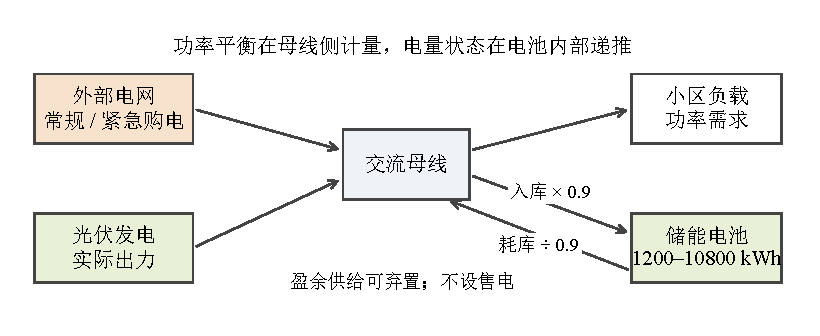
\includegraphics[width=.90\textwidth]{figures/energy_network.pdf}
\caption{微网结构与充放电效率的计量边界}\label{fig:energy_network}
\end{figure}

\subsection{问题任务}
题目以10分钟为调度间隔，每日共144个时段。问题1至3重复采用同一条日内电价曲线，问题4改用附件4的逐日实际价格。四问分别要求：

\textbf{问题1：}依据附件1给定的负荷、光伏预测与电价，制定单日购电和储能计划。日初日末电量均为6000 kWh，输出六个指定时段的购电量及4小时分组储能结果。

\textbf{问题2：}将日前计划扩展为全年连续运行。微网每天零时确定计划，实际缺额按当时交易电价的5倍补购；报告2月1日至12月31日的结果及四个指定日期。

\textbf{问题3：}使用0、6、12、18时发布的光伏预报调整未来执行安排，计入取消和追加购电的费用，并判断增加日内预报是否具有经济价值。

\textbf{问题4：}在附件4的波动电价下重新求解问题2、3，分别保存结果。未来价格何时可得会影响计划形成，我们把价格预测主方案与当天价格已知对照分开报告。

五份规定工作簿对应既定主模型；物理和因果性诊断用于核验，先知参照用于衡量信息与策略差距，门控、终端价值、预报融合及费用选型作为独立改进实验。

\section{问题分析}
四问使用同一物理基础与交易规则：功率在交流母线侧平衡，储能状态按单程效率递推，容量与功率受给定边界限制，常规购电按合同结算，缺额部分按5倍价格紧急补购。四问共用同一套母线功率平衡、储能递推与结算规则，差别只在信息条件：确定性输入、预测不确定性、日内预报更新与价格信息，我们按“先保证物理与结算可逐时核对、再逐个放宽信息条件”的顺序推进，每一步只作必要改动，使费用差异能够归因到明确来源。四问的继承关系、核心难点与所用方法汇总于表\ref{tab:analysis_map}，建模与评价流程见图\ref{fig:flow}。

\begin{table}[H]
\centering\footnotesize
\caption{四个问题的递进关系、核心难点与建模求解方法}
\label{tab:analysis_map}
\begin{tabular}{>{\raggedright\arraybackslash}p{0.9cm}>{\raggedright\arraybackslash}p{2.5cm}>{\raggedright\arraybackslash}p{4.0cm}>{\raggedright\arraybackslash}p{4.3cm}>{\raggedright\arraybackslash}p{2.0cm}}\toprule
问题 & 新增条件 & 本质与核心难点 & 建模与求解方法 & 主要输出\\\midrule
问题1 & 单日负荷、光伏与电价全部已知 & 本质是含储能的多时段能量调度；难点在功率与电量两组口径的衔接、同时充放电的排除，以及盈余供给的去向 & 确定性线性规划；HiGHS求解；用同成本等价变换代替0-1变量 & 指定时段购电量与4小时分组充放电量\\
问题2 & 负荷与光伏在计划时不可知；缺额按5倍价补购 & 本质是预测不确定性下的日前决策与跨日状态传递；难点是预测只能使用历史信息、风险必须提前计入目标 & 同星期与近7日均值预测，15个历史误差情景的两阶段线性规划，观测量反馈执行 & 2—12月总费用、紧急电量与事件清单\\
问题3 & 零时计划为结算基准；0、6、12、18时发布光伏预报 & 本质是分段结算下的滚动调整与采纳判断；难点是原计划不可改、每个时段只能结算一次 & 偏差变量的分段线性结算；滚动优化；同一情景下的费用门控 & 调整后购电量、调整费与紧急事件\\
问题4 & 附件4逐日波动价格，发布时点未声明 & 本质是价格信息可得性对计划的影响；难点是决策与结算必须使用不同价格设定 & 沿用前三问模型替换价格系数；价格预测主设定与当天价格已知对照 & 两套全年工作簿与价格信息价值度量\\
\bottomrule\end{tabular}
\end{table}

\textbf{问题1的分析：}问题1的输入曲线完全给定，本质是含储能的多时段能量调度：在储能动态、容量与功率边界、日初日末等电量约束下，在低价时段或光伏富余时段充电以替代高价时段购电，可归结为线性规划。问题有三个难点：量纲与口径衔接，功率以kW、电量以kWh计量，须统一到10分钟步长，且附件的时间标记存在10分钟错位，必须先固定离散化约定再建模；储能“充电—放电—存量”由效率耦合，若不加处理，最优解可能在同一时段同时充电与放电，虚增损耗而费用不变；盈余电量必须有明确去向，否则模型可借充放抵消消耗任意多余电能。针对上述难点，我们引入可弃置供给变量给出盈余的物理去向，并用保持储能状态与费用不变的等价变换证明主模型参数下总存在互斥最优解，从而无需引入0-1变量。所用理论工具为线性规划的等价变换。

\textbf{问题2的分析：}问题2把计划期延长为全年，核心变化在信息条件：附件2给出的是实际负荷与光伏，属于当天零时的未来量，直接作为已知输入即构成前视偏差。由此产生了两个难点。首先是预测：只能在历史信息下构造净负荷预测，并按时间顺序验证，避免用未来数据训练。其次是决策与风险的耦合：少购1 kWh省下的常规电费，可能不足以支付同量缺额的5倍紧急电费，所以应把未来缺额的可能代价提前计入目标。我们以历史误差轨迹构造情景，把这一权衡写成两阶段模型，其确定性等价形式仍为线性规划。第三个难点是跨日状态传递：日末电量必须来自实际执行结果，每日重置为6000 kWh等价于凭空注入或抽走能量。

\textbf{问题3的分析：}问题3在问题2之上增加两项条件：零时计划成为结算基准，日内只能调整未执行安排；0、6、12、18时各发布一次光伏预报，用于重排剩余时段。难点在于信息与合同的相互作用。一方面，新预报既可能降低缺额，也可能使原计划显得保守，是否调整取决于偏差费用与紧急风险的大小，须在同一费用口径下比较；另一方面，原计划一经签订即为基准，多个时点反复优化只能改变尚未执行的安排，且每个时段最终只结算一次，否则会重复计费。我们把三段结算写成关于偏差变量的分段线性函数，使调整问题不引入整数变量仍为线性规划；求解上采用“更新状态、优化未来、只实施前一段”的滚动优化，并设置费用门控，只有预计更便宜的候选安排才会被采纳。所用理论工具为模型预测控制的滚动时域原理。

\textbf{问题4的分析：}问题4把电价由重复曲线改为附件4的逐日波动价格。难点不在价格进入目标（它只是目标系数的变化），而在价格信息的时点：附件4只给出价格数值，并未声明何时发布。若按实际价格排计划，等价于假设零时即可预知当天价格，与问题2的因果性要求冲突；若按未知处理，又需要价格预测器，而题目未提供价格预报数据。我们因此把两种设定分开报告：主设定以历史同星期价格预测决策、按实际价格结算，与问题2保持同一信息约束；对照设定把当天价格视为零时已知，只放宽价格信息而保留负荷与光伏未知，用于量化价格信息的价值。低价充电、高价放电虽有经济动机，但容量边界、净负荷水平和价格预测误差会共同限制收益，该问题的结论因而必须与储能循环强度同时报告。

四问的递进关系体现为模型的可扩展性：问题2在问题1的物理约束上加入历史误差情景与执行反馈，问题3在问题2的跨日框架内加入合同偏差变量与日内更新，问题4只替换价格系数并区分信息设定。每后一问完整继承前一问的储能动态、边界条件与结算规则，新增部分均以独立基准对照检验。各项节省分别记账、不作叠加，也不以报告期费用反选主模型。
\begin{figure}[htbp]\centering
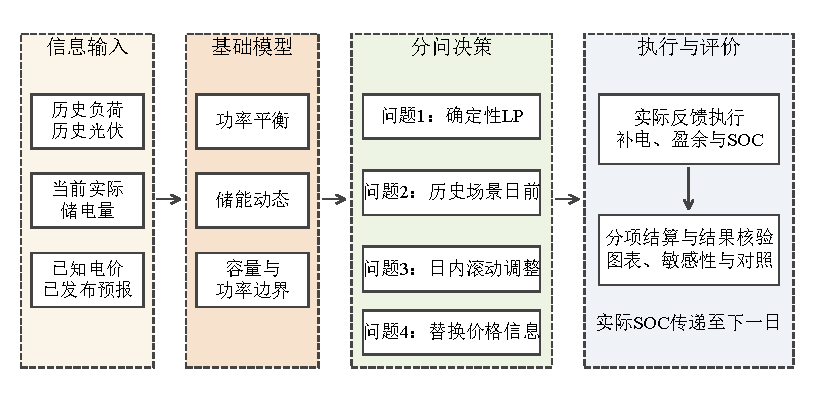
\includegraphics[width=.90\textwidth]{figures/study_flow.pdf}
\caption{四个问题的建模联系与计划—执行—评价流程}\label{fig:flow}
\end{figure}

\section{模型假设}
我们只保留进入模型或结果解释所必需的简化，列出以下九条假设，并说明每条的用途与依据。
\begin{enumerate}[label=（\arabic*）]
\item \textbf{时段内功率恒定：}每个10分钟时段内负荷、光伏、购电与充放电功率均视为常数，\(\dd=1/6\) h。（题目以10分钟为调度间隔，离散化后电量可由功率与步长相乘直接得到。）
\item \textbf{损耗只计充放电环节：}充电与放电效率均取常数0.9，线路损耗、自放电、温度变化和辅助耗电暂不计入。（题面只给出一个90\%的数值，我们取常数以与本模型的时段长度相容；第5.3.3节对效率的其他解释另作对照。）
\item \textbf{两侧计量口径分离：}充、放电功率按交流母线侧计量，储电量按电池内部计量；安全电量范围为1200--10800 kWh，最大充、放电功率均为5000 kW。（与题目给定边界一致，也避免把功率上限与容量上限混用。）
\item \textbf{同一时段不同时充放电：}执行阶段的反馈规则天然互斥，计划阶段则通过等价变换取互斥最优解。（同时充放只增加损耗、不改变费用，排除后既符合运行实际，又无需引入0-1变量。）
\item \textbf{外网只购不售：}不引入题面未给出的售电收益、并网功率上限或需量费；光伏富余与无法利用的已购电量允许弃置，已承诺电量仍按交易规则结算。（自行添加售电价格或接入容量会改变各方案的费用比较口径。）
\item \textbf{只使用决策时刻已可得的信息：}计划不得使用未来实际量；1月份用于初始化与方法选择，2月至12月用于报告，不用报告期实际费用反选主模型参数。（这是四问费用差异可归因于信息条件的前提。）
\item \textbf{储能状态跨日连续：}问题1两端电量均固定为6000 kWh；问题2至4仅在1月1日零时初始化一次，次日接续上一日的实际电量。（每日重置会凭空注入或抽走能量，与全年连续运行的要求不符。）
\item \textbf{合同偏差分段结算：}以零时合同为基准，履行量按原价、取消量按原价50\%付违约费、新增量按1.5倍原价购入，最终偏差只结算一次；原费不退且另罚的解释单列对照。（对应题面的三段措辞，两种文字解释在第9.2节分别重算。）
\item \textbf{执行优先保证负荷：}实际执行先满足负荷，再在容量与功率边界内决定充放电，不为追踪名义充电功率额外购买紧急电；供电不足部分按实际交易价格的5倍结算。（5倍价对应题面规定，该规则只依赖当前观测量，是可实施的因果策略。）
\end{enumerate}

效率在第（2）项中按单程解释，故回路效率为0.81。例如母线侧输入100 kWh，内部只增加90 kWh；母线侧输出100 kWh，内部减少约111.1 kWh。我们把这一区别只放在状态动态中处理，输出电量不再重复扣除效率。

\section{符号说明}
令日期索引\(d=1,\ldots,365\)，报告期为\(\mathcal D=\{32,\ldots,365\}\)；时段索引\(t=1,\ldots,144\)，\(t=1\)对应0:00--0:10，状态\(E_{d,t}\)为第\(t\)个时段结束时的电量，\(E_{d,0}\)为零时电量。发布时刻\(k\in\{0,6,12,18\}\)，误差场景索引为\(s\)。单日推导省略日期下标。我们按集合与索引、输入与预测、设备参数、决策变量、费用与评价五类分组列出符号，同类量采用统一的字母约定：\(P\)表示功率、\(E\)表示电量、\(\lambda\)表示电价、\(C\)表示费用。
\begin{center}\small
\begin{longtable}{p{3.7cm}p{8.0cm}p{2.0cm}}
\toprule 符号 & 说明 & 单位\\\midrule\endfirsthead
\toprule 符号 & 说明 & 单位\\\midrule\endhead
\multicolumn{3}{l}{\textbf{（一）集合与索引}}\\
\(\mathcal D\) & 报告期日期集合，即第32日至第365日 & --\\
\(d,t,k,s\) & 日期、时段、预报发布时刻、误差场景索引 & --\\
\(\mathcal I_{d,0}\) & 第\(d\)日零时可用的信息集合 & --\\
\(p^0,g^{\mathrm{keep}},g^*\) & 原计划、当前执行安排、候选安排的功率向量 & kW\\
\midrule
\multicolumn{3}{l}{\textbf{（二）输入与实际量}}\\
\(P_{\mathrm{load},d,t},P_{\mathrm{pv},d,t}\) & 实际负载功率、实际光伏功率 & kW\\
\(\widehat P_{\mathrm{load},d,t}\) & 当日零时形成的负载预测 & kW\\
\(\widehat P_{\mathrm{pv},d,t}^{(k)}\) & 发布时刻\(k\)对应的光伏预测 & kW\\
\(n_{d,t},\widehat n_{d,t}^{(k)}\) & 实际净负荷、预测净负荷，均为负载减光伏 & kW\\
\(n_{d,t,s}^{(k)}\) & 场景净负荷 & kW\\
\(\lambda_{d,t},\widehat\lambda_{d,t}\) & 实际交易电价、日前预测电价 & 元/kWh\\
\midrule
\multicolumn{3}{l}{\textbf{（三）设备与时间参数}}\\
\(\eta_c,\eta_d\) & 充电、放电效率，均为0.9 & --\\
\(\dd\) & 时间步长，等于1/6 & h\\
\(\Emin,\Emax\) & 允许储电量下限1200、上限10800 & kWh\\
\(P_{\max}\) & 最大充电、放电功率，均为5000 & kW\\
\midrule
\multicolumn{3}{l}{\textbf{（四）决策与派生变量}}\\
\(P_{\mathrm{grid},d,t}^{0}\) & 零时原始计划购电功率 & kW\\
\(P_{\mathrm{grid},d,t}\) & 最终生效的常规购电功率，不含紧急补电 & kW\\
\(P_{\mathrm{ch},d,t},P_{\mathrm{dis},d,t}\) & 母线侧充电输入、放电输出功率 & kW\\
\(E_{d,t}\) & 实际或模型中明确指定的边界储电量 & kWh\\
\(P_{\mathrm{em},d,t}\) & 实际紧急购电功率 & kW\\
\(P_{\mathrm{sp},d,t}\) & 弃光或未利用的已付费供给功率 & kW\\
\(u_{d,t,s}\) & 计划模型中的场景缺额补救变量 & kW\\
\(y_{d,t}^{+},y_{d,t}^{-}\) & 相对零时计划的上调、下调功率 & kW\\
\midrule
\multicolumn{3}{l}{\textbf{（五）费用与评价指标}}\\
\(C_{\mathrm{total}}\) & 报告期实际总费用 & 元\\
\(v_d,\gamma\) & 电池内部单位库存价值、无量纲调节系数 & 元/kWh，--\\
\(\widehat V_k(g)\) & 更新时刻对剩余安排的预计反馈费用 & 元\\
\bottomrule
\end{longtable}\end{center}
\par\textbf{计划状态与实际状态：}
优化阶段的充放电变量与状态描述名义储能计划；实际执行时，以反馈规则重新计算充放电与状态。必要时我们分别加上标\(\mathrm{pl}\)和\(\mathrm{act}\)。场景缺额\(u\)只是优化目标中的风险代理量，不与实际紧急功率\(P_{\mathrm{em}}\)混用。

\par\textbf{费用口径：}
我们定义原计划费用\(C_0\)、上调费用\(C_+\)、下调净费用\(C_-\)与实际紧急费用\(C_{\mathrm{em}}\)，总费用为
\begin{equation}\label{eq:total}
C_{\mathrm{total}}=C_0+C_++C_-+C_{\mathrm{em}}.
\end{equation}

主口径中\(C_-\le0\)，表示先扣回取消电量的全额原电费，再收取50\%违约费后的净减少额。违约费用本身仍非负。保留原费的对照口径中\(C_-\ge0\)。
\par\textbf{储能利用指标：}
为统一表征储能使用强度，定义基于9600 kWh可用容量的能量吞吐等效循环次数
\begin{equation}\label{eq:cycle}
N_{\mathrm{eq}}=\frac{\sum_{d\in\mathcal D,t}\bigl(\eta_cP_{\mathrm{ch},d,t}+P_{\mathrm{dis},d,t}/\eta_d\bigr)\dd}{2(\Emax-\Emin)}.
\end{equation}

它只刻画运行强度，并不等同于寿命模型里的电池循环计数，我们也没有据此假设折旧成本。

\section{问题1的模型建立与求解}
\subsection{模型准备}
\subsubsection{附件读取与时段对齐}
四份附件的规模为：附件1共144个时段，附件2有365天负荷与实际光伏，附件3有1460条整点预报，附件4有365组日内电价。读取时先核对日期、时段与预报发布顺序，再检查维度、缺失值和非负性，四份附件全部通过。

附件1电价介于0.3713--1.3952元/kWh，附件4介于0.0076--1.7936元/kWh。

原始输入的时间字段从0:10到次日0:00，共144个值；我们按区间末端标记解释，即0:10对应0:00--0:10的平均功率。附件5的部分模板却从0:10--0:20开始，末行延伸到次日0:10，与完整自然日边界存在10分钟错位。输出保留原有工作表名称及字段结构，将144个时段标签统一为0:00--0:10至23:50--24:00，不平移数值，这是明确的时间离散化约定；若另有权威时标解释，应据此重新映射并重新计算。

对功率\(P_t\)，时段电量为\(q_t=P_t\dd\)。例如4小时分组包含24个时段，其充电量等于24个充电功率之和乘以\(1/6\)。输出工作簿以kWh计量，填表前统一做这一步换算。

\subsection{模型建立}
\subsubsection{决策变量与目标函数}
单日模型的主要变量为\(P_{\mathrm{grid},t}\)、\(P_{\mathrm{ch},t}\)、\(P_{\mathrm{dis},t}\)与\(E_t\)，并引入非负盈余处理量\(P_{\mathrm{sp},t}\)。购电只发生在外网方向，目标函数为
\begin{equation}\label{eq:q1obj}
\min C_1=\sum_{t=1}^{144}\lambda_t P_{\mathrm{grid},t}\dd.
\end{equation}

价格与时长都是已知系数，目标对购电功率线性。题目未给定的寿命费、售电收益与峰值需量费不进入本次计算。

\subsubsection{功率平衡与储能边界}
母线功率平衡及储能动态分别为
\begin{align}
P_{\mathrm{grid},t}+P_{\mathrm{pv},t}+P_{\mathrm{dis},t}
&=P_{\mathrm{load},t}+P_{\mathrm{ch},t}+P_{\mathrm{sp},t},\label{eq:balance}\\
E_t&=E_{t-1}+\eta_cP_{\mathrm{ch},t}\dd-\frac{P_{\mathrm{dis},t}\dd}{\eta_d}.\label{eq:soc}
\end{align}

式\eqref{eq:balance}使富余供给具有明确去向；消去\(P_{\mathrm{sp},t}\ge0\)后，可等价写为供给不低于负荷和充电需求的不等式。式\eqref{eq:soc}中的充电量需乘效率，放电输出需除以效率，且始终使用\(E_{t-1}\)与\(E_t\)连接相邻边界。
\begin{align}
1200\le E_t\le10800,&\qquad t=0,\ldots,144,\label{eq:boundE}\\
0\le P_{\mathrm{ch},t}\le5000,&\qquad0\le P_{\mathrm{dis},t}\le5000,\label{eq:boundP}\\
P_{\mathrm{grid},t}\ge0,&\qquad P_{\mathrm{sp},t}\ge0,\label{eq:positive}\\
E_0=E_{144}&=6000.\label{eq:cyclic}
\end{align}

上述目标、等式和不等式均为线性表达式，故在暂不添加乘积互斥约束的情况下，可构成线性规划\cite{boyd}。将式\eqref{eq:q1obj}与约束\eqref{eq:balance}--\eqref{eq:cyclic}汇总，问题1的模型为
\begin{equation}\label{eq:q1model}
\left\{\begin{aligned}
\min\quad & C_1=\sum_{t=1}^{144}\lambda_tP_{\mathrm{grid},t}\dd\\
\text{s.t.}\quad
& P_{\mathrm{grid},t}+P_{\mathrm{pv},t}+P_{\mathrm{dis},t}=P_{\mathrm{load},t}+P_{\mathrm{ch},t}+P_{\mathrm{sp},t},\\
& E_t=E_{t-1}+\eta_cP_{\mathrm{ch},t}\dd-P_{\mathrm{dis},t}\dd/\eta_d,\\
& \Emin\le E_t\le\Emax,\\
& 0\le P_{\mathrm{ch},t}\le P_{\max},\qquad0\le P_{\mathrm{dis},t}\le P_{\max},\\
& P_{\mathrm{grid},t}\ge0,\qquad P_{\mathrm{sp},t}\ge0,\\
& E_0=E_{144}=6000,
\end{aligned}\right.\qquad t=1,\ldots,144
\end{equation}

其中购电功率、充放电功率与储电量为决策变量，负荷、光伏与电价为已知系数，模型规模为\(4\times144=576\)个连续变量。

\subsubsection{线性性质与同时充放电处理}
电价为正并不能自动保证LP最优解不同时充放电；我们在允许零成本弃置、效率为常数的条件下，给出一个保持状态与费用的显式消除方法。设某时段\(c=P_{\mathrm{ch},t}>0\)、\(p=P_{\mathrm{dis},t}>0\)，取
\begin{equation}\label{eq:remove}
\delta=\min\left(c,\frac{p}{\eta_c\eta_d}\right),\qquad
c'=c-\delta,\quad p'=p-\eta_c\eta_d\delta.
\end{equation}

按上式调整后，至少有一个新功率为零，储能状态增量保持不变。购电功率保持不变，多出来的净供给\((1-\eta_c\eta_d)\delta\)交给弃电变量吸收即可：费用不变，各功率上界也照旧满足。因此，至少存在一个不同时充放电、费用相同的最优解。程序按式\eqref{eq:remove}处理求解结果，并核验所有时段确实互斥。

若将来引入弃电上限、售电收益、负价格或额外运行机制，上述等价性需重新判断；必要时可引入二元变量\(z_t\)，设置\(P_{\mathrm{ch},t}\le5000z_t\)、\(P_{\mathrm{dis},t}\le5000(1-z_t)\)，形成混合整数线性规划。我们的主模型不需要二元变量。

\subsection{模型求解与结果分析}
\subsubsection{稀疏线性规划求解}
输入数据读取后，按变量顺序组成稀疏约束矩阵，调用\texttt{scipy.optimize.linprog}并设置\texttt{method='highs'}\cite{scipy,highs}，检查求解成功标志、等式残差和不等式余量，再输出逐时功率、时段电量与分组汇总。固定初始状态后，消去盈余变量和固定为零的紧急变量，核心问题具有\(4\times144=576\)个连续变量。

\subsubsection{单日购电与储能调度}
单日最优购电量为\textbf{59482.70 kWh}，购电费用为\textbf{35126.95元}。指定结果见表\ref{tab:q1_purchase}和表\ref{tab:q1_storage}。
\begin{table}[H]\centering\small
\caption{问题1指定时段常规购电量（电量单位：kWh）}
\label{tab:q1_purchase}
\begin{tabular}{lrlrlr}\toprule
时段 & 购电量 & 时段 & 购电量 & 时段 & 购电量 \\\midrule
10:00--10:10 & 0.00 & 12:00--12:10 & 480.41 & 14:00--14:10 & 0.00 \\
16:00--16:10 & 445.43 & 18:00--18:10 & 531.89 & 20:00--20:10 & 0.00 \\
\midrule
\multicolumn{3}{l}{全天常规购电量：59482.70 kWh} & \multicolumn{3}{r}{全天总费用：35126.95 元}\\
\bottomrule\end{tabular}\end{table}

\begin{table}[H]\centering\small
\caption{问题1储能充放电量与边界电量（单位：kWh）}
\label{tab:q1_storage}
\begin{tabular}{lrrlrr}\toprule
时段 & 充电量 & 放电量 & 时段 & 充电量 & 放电量\\\midrule
0:00--4:00 & 4500.00 & 0.00 & 4:00--8:00 & 833.33 & 6365.84 \\
8:00--12:00 & 4787.96 & 1703.00 & 12:00--16:00 & 5286.04 & 91.10 \\
16:00--20:00 & 0.00 & 5780.13 & 20:00--24:00 & 5333.33 & 2859.87 \\
\midrule\multicolumn{3}{l}{0:00储电量：6000.00} & \multicolumn{3}{r}{24:00储电量：6000.00}\\
\bottomrule\end{tabular}\end{table}


购电表列出六个指定10分钟时段，储能表按4小时汇总。值得核对的是12:00--12:10：该段仍购入约480 kWh，而10:00、14:00和20:00的指定时段无需购电；日间购电与储能补充需求及后续价差有关，并非异常。

全天充电约2.074万kWh、放电约1.680万kWh，差额约3941 kWh。日初日末电量相等时，\(Q_{\mathrm{dis}}=\eta_c\eta_d Q_{\mathrm{ch}}\)，本次计算满足该关系，差额可归为充放电损耗。

4小时分组里同时出现充电和放电，只是说明组内不同10分钟时段发生了两类操作，并非同一时段两者并行。

\begin{figure}[htbp]\centering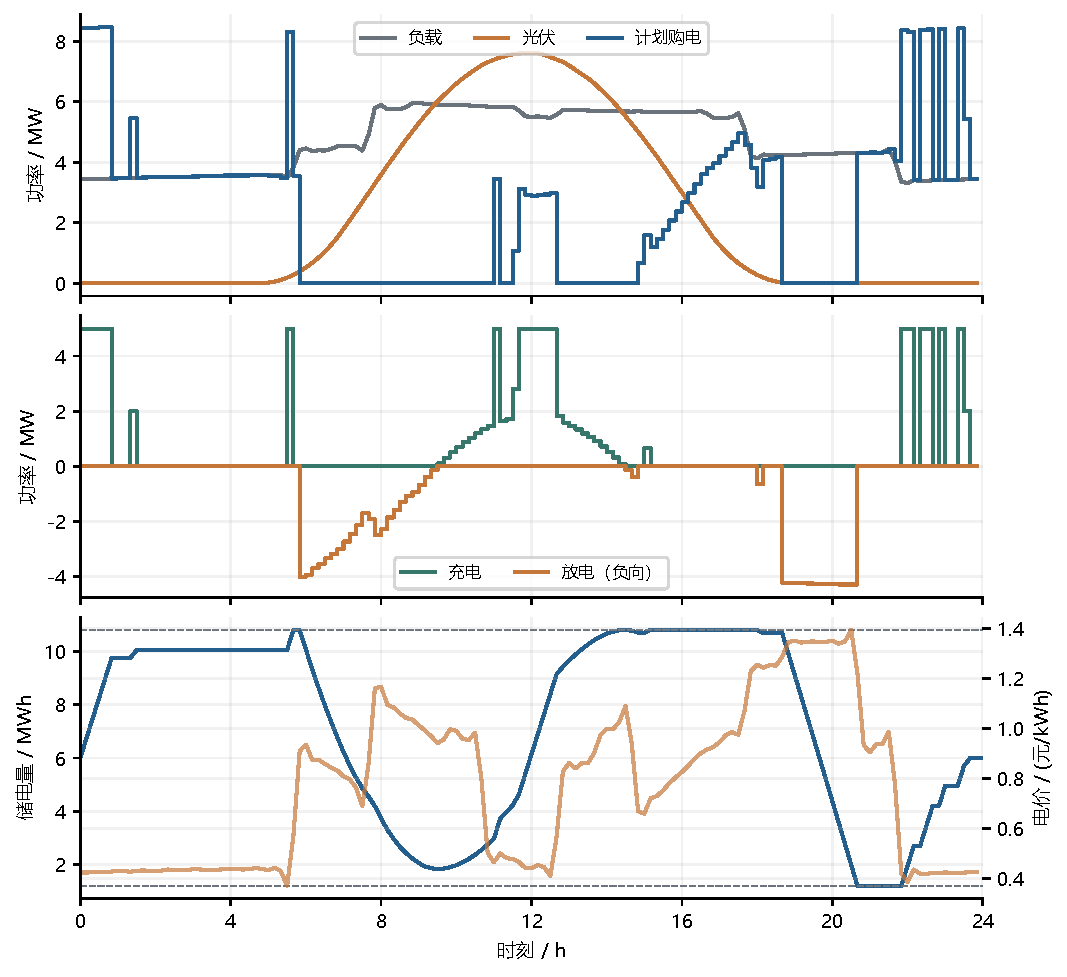
\includegraphics[width=.85\textwidth]{figures/q1_dispatch.pdf}\caption{附件1算例中，储能在容量与功率边界内转移购电需求}\label{fig:q1}\end{figure}
图\ref{fig:q1}中储电量多次贴近边界，可见低价购电与高价放电同时受9600 kWh可用容量和5000 kW功率上限的约束。同样输入下若不配储能、直接购买正净负荷，费用为48052.05元，本方案节省12925.10元、约26.9\%。该降幅只对应附件1单日算例，全年节省率见问题2。

\subsubsection{效率解释的敏感性}
我们把“充放电效率90\%”解释为两侧单程各0.9。为检验该解释的影响，以同一附件1独立构造LP，分别改变效率分配，其余约束与两端电量保持一致。若把0.9视为回路效率并对称分配，费用约为33801.50元，比主设定低3.77\%。仅在充电或放电侧计损耗时，费用分别约33416.53元和34168.61元。精确结果见附录D表\ref{tab:review_efficiency}。

相同的回路效率仍可能算出不同费用，因为两侧效率还决定了给定内部容量与母线功率下实际可充、可放的电量。图\ref{fig:efficiency_interpretation}显示效率口径对结果有实质影响，主计算维持两侧各0.9。

\begin{figure}[htbp]\centering
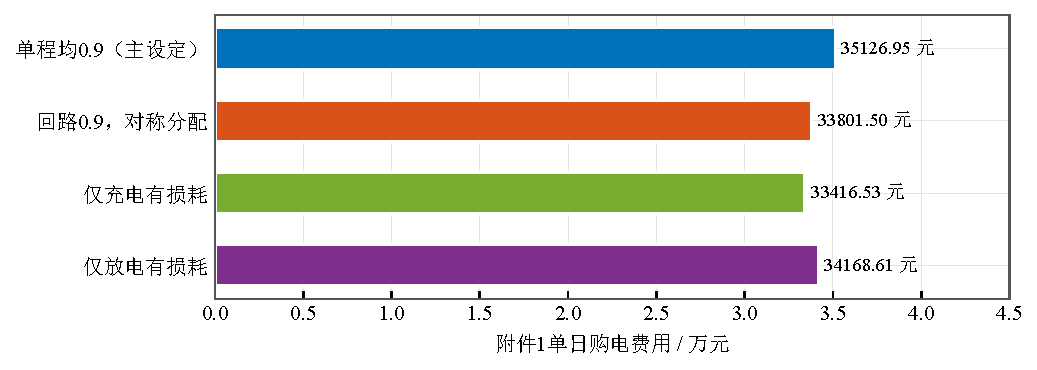
\includegraphics[width=.90\textwidth]{figures/efficiency_interpretation.pdf}
\caption{效率解释改变单日费用，全部比较保持容量与两端电量一致}\label{fig:efficiency_interpretation}\end{figure}

\section{问题2的模型建立与求解}
\subsection{数据特征与历史预测}
\begin{figure}[htbp]\centering
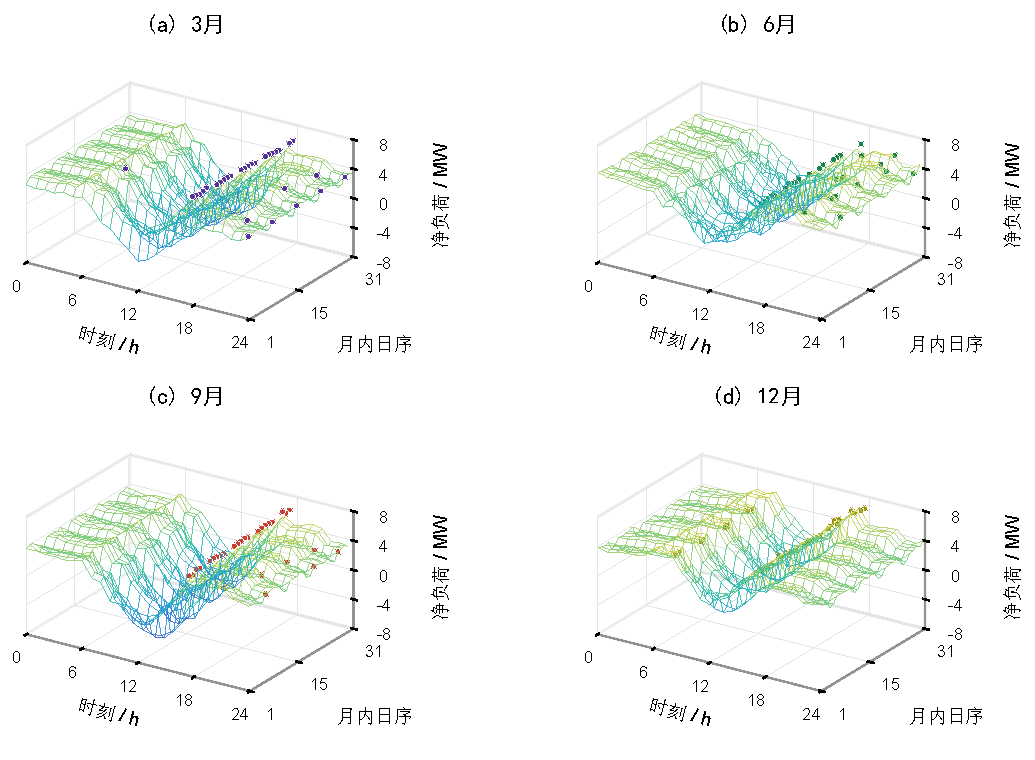
\includegraphics[width=.90\textwidth]{figures/input_profiles.pdf}
\caption{四个代表月份的实际净负荷曲面，散点标出每日峰值（统一纵轴尺度）}\label{fig:input_profiles}
\end{figure}

图\ref{fig:input_profiles}以日序、时刻和净负荷展示3、6、9、12月的实际变化。净负荷为负荷减光伏；细网格连接逐小时抽取的10分钟观测并保留末时段，散点取每日全部144时段的最大值。四图共用纵轴范围，网格不代表回归拟合。图示仅作事后描述，不作为零时已知输入；月内平均曲线另存于插图文件夹。季节差异仍需通过历史信息逐日跟踪。

验证按时间顺序进行，不随机打乱训练与验证数据\cite{forecast}。候选方法有前一日持久性、3日和7日移动平均、14日指数加权平均，以及过去最多四个同星期日期的均值，指数权重取\(\exp(-j/5)\)，\(j\)为距最新一天的天数。我们用1月15日至31日的逐日历史预测MAE选定方法，2月1日起固定方法、滚动更新历史输入；1月运行的热启动统一用持久性方法，1月1日历史不足时以附件1曲线作初始先验，保证1月的运行不依赖事后选型。

对任一待预测序列\(x_{d,t}\)，选出的同星期预测与7日均值分别为
\begin{align}
\widehat x_{d,t}^{\mathrm{week}}&=\frac{1}{|\mathcal L_d|}\sum_{\ell\in\mathcal L_d}x_{d-\ell,t},\quad \mathcal L_d=\{7,14,21,28\}\cap[1,d-1],\label{eq:week}\\
\widehat x_{d,t}^{\mathrm{mean7}}&=\frac{1}{m_d}\sum_{\ell=1}^{m_d}x_{d-\ell,t},\quad m_d=\min(7,d-1).\label{eq:mean}
\end{align}

历史不足一周时，同星期方法退化为最近七日的平均。各方法评价见表\ref{tab:forecast}；WAPE用绝对误差总和除以实际值总和，避免夜间光伏零值让MAPE失去定义。
\begin{table}[H]
\centering\small
\caption{历史预测误差（1月验证，2--12月测试）}
\label{tab:forecast}
\begin{tabular}{lrrrrr}\toprule
变量 & 选定方法 & 验证MAE & 测试MAE & 测试RMSE & 测试WAPE \\\midrule
负载/kW & 同星期均值 & 117.84 & 188.88 & 262.06 & 4.09\% \\
光伏/kW & 7日移动均值 & 96.18 & 153.40 & 303.86 & 6.45\% \\
电价/(元/kWh) & 同星期均值 & 0.03 & 0.0489 & 0.0696 & 6.45\% \\
\bottomrule\end{tabular}
\end{table}


1月验证选中了负载、价格的同星期均值和光伏的7日均值，与“负荷和电价按星期重复”的日常经验相符，但仅一个月的验证不足以证明该规律全年稳定。表\ref{tab:forecast}中的误差大小还要放到费用模型里检验：电量紧张时，几个连续时段的偏差可能比孤立的同量偏差更昂贵。
\begin{figure}[htbp]\centering
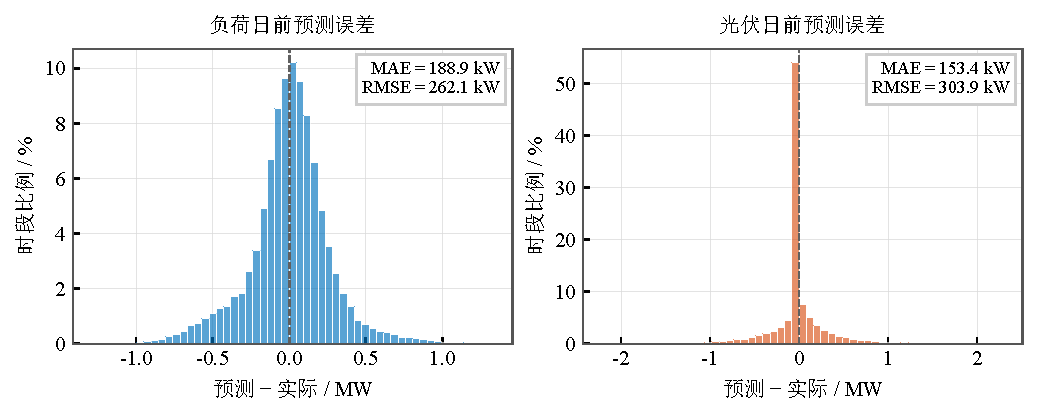
\includegraphics[width=.90\textwidth]{figures/forecast_errors.pdf}
\caption{报告期日前预测误差分布：误差较小的主体之外仍有偏离较大的时段}\label{fig:forecast_errors}
\end{figure}

图\ref{fig:forecast_errors}统计报告期全部48096个时段，误差定义为预测减实际，纵轴是各分组的时段占比。零误差附近的高度集中主要来自夜间——光伏此时接近零，白天时段的误差仍分布在更宽的范围，不能由该图推断白天预测同样准确。缺额风险还需要在费用目标中单独处理。

\subsection{模型建立}
\subsubsection{历史误差场景与费用目标}
令\(\varepsilon_{j,t}^{(k)}=n_{j,t}-\widehat n_{j,t}^{(k)}\)为过去日期\(j\)相同发布时刻的净负荷预测误差。主模型采用过去\(H=14\)天误差轨迹，加上一个零误差场景，得到
\begin{equation}\label{eq:scenario}
n_{d,t,s}^{(k)}=\widehat n_{d,t}^{(k)}+\varepsilon_{j_s,t}^{(k)},\qquad
\varepsilon_{j_0,t}^{(k)}=0.
\end{equation}

场景保留历史日内误差轨迹的形状并等权使用，成熟阶段场景数\(S=15\)；这是近期误差经验分布的近似，不宣称覆盖全部未来误差，也不额外假定正态分布，其窗口敏感性见第9节。

一次少购电所省下的常规电费，可能不足以支付同量缺额的5倍紧急电费。日前模型因而同时选择共同购电计划、共同名义充放电轨迹及各场景缺额变量\(u_{d,t,s}\)，目标为
\begin{equation}\label{eq:q2obj}
\min J_d=\sum_t\lambda_tP_{\mathrm{grid},d,t}^{0}\dd
+\frac1S\sum_s\sum_t5\lambda_tu_{d,t,s}\dd.
\end{equation}

对所有\(t,s\)设置
\begin{align}
P_{\mathrm{grid},d,t}^{0}+P_{\mathrm{dis},d,t}^{\mathrm{pl}}-P_{\mathrm{ch},d,t}^{\mathrm{pl}}+u_{d,t,s}
&\ge n_{d,t,s}^{(0)},\label{eq:scenarioineq}\\
u_{d,t,s}&\ge0.\label{eq:u}
\end{align}

名义储能满足式\eqref{eq:soc}--\eqref{eq:boundP}，以实际\(E_{d,0}^{\mathrm{act}}\)起步，日末电量自由。共同计划是第一阶段变量，场景缺额是第二阶段变量；各场景没有分别递推自己的电池状态。整理后，问题2的日前模型为
\begin{equation}\label{eq:q2model}
\left\{\begin{aligned}
\min\quad & J_d=\sum_t\lambda_tP_{\mathrm{grid},d,t}^{0}\dd+\frac1S\sum_s\sum_t5\lambda_tu_{d,t,s}\dd\\
\text{s.t.}\quad
& P_{\mathrm{grid},d,t}^{0}+P_{\mathrm{dis},d,t}^{\mathrm{pl}}-P_{\mathrm{ch},d,t}^{\mathrm{pl}}+u_{d,t,s}\ge n_{d,t,s}^{(0)},\quad\forall t,s,\\
& \text{式\eqref{eq:soc}--\eqref{eq:boundP}（共同名义储能与功率边界）},\\
& E_{d,0}^{\mathrm{pl}}=E_{d,0}^{\mathrm{act}},\qquad u_{d,t,s}\ge0,\\
& P_{\mathrm{grid},d,t}^{0}=\pi_t(\mathcal I_{d,0},E_{d,0}^{\mathrm{act}}),
\end{aligned}\right.\qquad t=1,\ldots,144,\ s=1,\ldots,S
\end{equation}

最后一式表示计划只能由零时已有信息与当前电量决定，是模型的可实施性约束\cite{birge}。

仅保留一个零误差场景时，模型退化为点预测基准，供给通常由较便宜的常规购电满足。

需要指出，\(J_d\)只是计划阶段的风险代理而非实际费用：运行时电池按当期供需反馈，实际紧急量未必等于LP中的\(u\)。因此最终费用由连续反馈仿真单独结算，第9节再用时间配对诊断、窗口敏感性和反馈对照核查这项近似的量级。

\subsubsection{实际反馈与跨日状态传递}
在执行时段\(t\)，以生效常规功率和实际净负荷计算
\begin{equation}\label{eq:residual}
R_{d,t}=P_{\mathrm{grid},d,t}+P_{\mathrm{pv},d,t}-P_{\mathrm{load},d,t}.
\end{equation}

若\(R_{d,t}\ge0\)，取
\begin{equation}\label{eq:chargefeedback}
P_{\mathrm{ch},d,t}=\min\left\{R_{d,t},P_{\max},\frac{\Emax-E_{d,t-1}}{\eta_c\dd}\right\},\quad
P_{\mathrm{dis},d,t}=P_{\mathrm{em},d,t}=0,
\end{equation}
并令\(P_{\mathrm{sp},d,t}=R_{d,t}-P_{\mathrm{ch},d,t}\)。若\(R_{d,t}<0\)，则
\begin{align}
P_{\mathrm{dis},d,t}&=\min\left\{-R_{d,t},P_{\max},\frac{\eta_d(E_{d,t-1}-\Emin)}{\dd}\right\},\label{eq:disfeedback}\\
P_{\mathrm{em},d,t}&=-R_{d,t}-P_{\mathrm{dis},d,t},\quad P_{\mathrm{ch},d,t}=P_{\mathrm{sp},d,t}=0.\label{eq:emfeedback}
\end{align}
再依据式\eqref{eq:soc}更新实际状态。该反馈规则不为维持原定充电功率而紧急购电，而是优先满足实际负荷；其计算只依赖当前已观测量。紧急电量和实际费用为
\begin{align}
Q_{\mathrm{em},d}&=\sum_tP_{\mathrm{em},d,t}\dd,\label{eq:emenergy}\\
C_d&=\sum_t\lambda_tP_{\mathrm{grid},d,t}^{0}\dd+\sum_t5\lambda_tP_{\mathrm{em},d,t}\dd.\label{eq:q2cost}
\end{align}

次日初值为\(E_{d+1,0}^{\mathrm{act}}=E_{d,144}^{\mathrm{act}}\)。主方案从1月1日连续运行，2月1日零时实际电量约9341 kWh，年末约1553 kWh。

6000 kWh只在1月1日零时使用一次；若每天恢复到该值，相当于每天凭空补入或移走一部分能量。
\begin{figure}[htbp]\centering
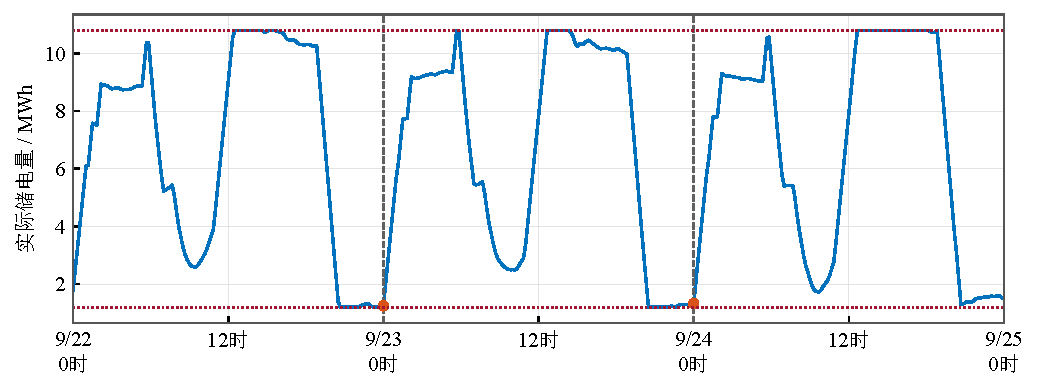
\includegraphics[width=.90\textwidth]{figures/soc_continuity.pdf}
\caption{9月22—24日实际储电量连续衔接，日初不重置为6000 kWh}\label{fig:soc_continuity}
\end{figure}

\subsubsection{终端库存价值的独立修正}
不强制日末恢复初值，可能使短时域模型过早耗用库存。为此在日前目标中加入线性终端价值项：
\begin{equation}\label{eq:terminal}
\min J_d^{\mathrm{term}}=J_d-v_dE_{d,144}^{\mathrm{pl}},\qquad
v_d=\gamma\eta_d\overline{\widehat\lambda}_{d+1}.
\end{equation}

其中\(v_d\)单位为元/电池内部kWh；\(\overline{\widehat\lambda}_{d+1}\)是零时可得的次日平均价估计。重复电价直接采用已知曲线均价；波动电价使用次日对应的过去同星期价格，\textbf{不使用当天尚未观测的价格}；该线性项仅改变目标系数，不增加整数变量，也不改变跨日实际状态传递。

\(\gamma\)从\(\{0,0.5,1,1.5\}\)里选，办法很直接：每个候选都从1月15日的实际电量出发模拟到1月31日，比谁的“现金费用减去期末库存价值”更低，库存价值按附件1零至6时平均电价乘\(\eta_d\)计算。2月起冻结选出的\(\gamma\)，接着1月末的实际电量继续往下跑，1月的历史不回头改。
各候选参数的1月份库存修正费用见附录D表\ref{tab:terminal_validation}，冻结参数后的报告期结果如下。

\begin{table}[H]\centering\small
\caption{所选终端价值仅在波动电价日前方案中降低报告期费用}\label{tab:terminal_results}
\begin{tabular}{lrrrr}\toprule
方案 & $\gamma$ & 总费用/元 & 紧急电量/kWh & 期末SOC/kWh \\\midrule
重复电价：原模型 & 0.00 & 13863865.66 & 85480.79 & 1552.80 \\
重复电价：终端价值 & 0.00 & 13863865.66 & 85480.79 & 1552.80 \\
波动电价：原模型 & 0.00 & 14621415.17 & 83563.75 & 1548.85 \\
波动电价：终端价值 & 0.50 & 14608967.43 & 83551.31 & 1545.92 \\
\bottomrule\end{tabular}\end{table}


重复电价选中\(\gamma=0\)，即验证期不支持额外的终端奖励。波动电价选中\(\gamma=0.5\)，报告期少支出约1.24万元。这说明库存价值值得继续考察，但单个系数能否普遍适用，证据还不够。

终端价值只是对次日价值的线性近似，并未真正求解未来48小时，因此不作为收入从电费中扣减。

\subsection{模型求解与结果分析}
\subsubsection{可实施策略与未来已知参照}
定义零时信息集\(\mathcal I_{d,0}\)包含截至前一日完成的观测及当时已知的交易规则，要求\(P_{\mathrm{grid},d,t}^{0}=\pi_t(\mathcal I_{d,0},E_{d,0}^{\mathrm{act}})\)。附件2的当日实际曲线不属于该集合。可实施的主策略按日期向前推进；当日先知参照则刻意放宽信息限制，在零时直接输入当天实际负荷、光伏和相应价格，逐日求解确定性LP，但仍只优化当天且连续传递实际SOC。

另设一条对照：把2--12月的全部实际曲线一次性交给一个全期LP，期初、期末电量分别钉在对应主策略的水平，得到全期先知的成本下界。物理约束相同，先知可以用便宜的常规电替代紧急电，所以这个下界不会高于主策略费用；但它需要整个报告期的未来信息，优化时域也不同，不是可执行的方案。
\begin{table}[H]\centering\small
\caption{先知参照费用更低，比较仍须区分信息与库存边界（费用/元，电量/kWh）}\label{tab:information_benchmark}
\begin{tabular}{lrrrr}\toprule
信息与策略 & 总费用 & 紧急电量 & 期初SOC & 期末SOC \\\midrule
重复价：可实施日前 & 13863865.66 & 85480.79 & 9340.95 & 1552.80 \\
重复价：当日先知 & 12250938.36 & 0.00 & 9340.95 & 1200.00 \\
重复价：全期先知 & 12226776.72 & 0.00 & 9340.95 & 1552.80 \\
波动价：可实施日前 & 14621415.17 & 83563.75 & 9218.19 & 1548.85 \\
波动价：当日先知 & 12838166.23 & 0.00 & 9218.19 & 1200.00 \\
波动价：全期先知 & 12779898.60 & 0.00 & 9218.19 & 1548.85 \\
\bottomrule\end{tabular}\end{table}


重复电价下，全期先知费用约1222.68万元，比主策略低约163.71万元。这笔差额里混着预测信息、风险代理与反馈策略三方面的影响，只能当作参考上界，而不是严格的完全信息期望价值。当日先知只优化当天，期末库存与主策略仍有差异，两者不能直接比较。

波动电价的全期参照还放宽了价格信息；第8.2.1节的对照只放宽价格信息，两者作用不同。

\subsubsection{四个指定日期的结果}
四个指定日期的完整指标见表\ref{tab:q2_daily_summary}。指定时段购电量、4小时分组储能量及紧急事件完整列于附录C；问题2无日内调整，原计划量与最终常规购电量相同，全天总费用含实际紧急补电费。
\begin{table}[H]
\centering\small
\caption{问题2典型日购电与费用汇总}
\label{tab:q2_daily_summary}
\begin{tabular}{lrrrr}\toprule
日期 & 原计划/kWh & 调整后/kWh & 紧急/kWh & 总费用/元 \\\midrule
03-20 & 68991.98 & 68991.98 & 0.00 & 41918.85 \\
06-21 & 36523.04 & 36523.04 & 0.00 & 21502.49 \\
09-23 & 68842.58 & 68842.58 & 1094.87 & 49439.26 \\
12-21 & 98355.39 & 98355.39 & 0.00 & 63456.61 \\
\bottomrule\end{tabular}
\end{table}


指定日期中，6月21日常规购电约3.65万kWh，12月21日约9.84万kWh，外购需求差异较大。9月23日约1095 kWh紧急电量中，约1018 kWh集中在20:20--21:30，发生在光伏退出后的晚间负荷阶段；紧急费约6905元，占该日总费近14\%。

其余三个指定日期没有发生紧急事件；作为典型日，它们不代表所在月份整月都没有缺额。

\subsubsection{报告期费用与紧急购电}
报告期覆盖334天、48096个时段，总费约1386.39万元，其中计划费约1337.62万元、紧急费约48.77万元。紧急购电共约8.55万kWh，分布在105天的733个时段。
\begin{table}[H]
\centering\small
\caption{计入缺额风险后，常规购电增加而总费用下降（本算例）}
\label{tab:risk}
\begin{tabular}{lrrrr}\toprule
方案 & 计划电量/万kWh & 紧急电量/kWh & 紧急天数 & 总费用/万元 \\\midrule
点预测基准 & 1999.72 & 674346.09 & 272 & 1599.85 \\
问题2 & 2179.10 & 85480.79 & 105 & 1386.39 \\
\bottomrule\end{tabular}
\end{table}


与点预测基准比较，风险代理方案多购约179万kWh常规电，少购约59万kWh紧急电，净节省约213万元。提前计入缺额代价，在本算例中比运行后才统计紧急费更有效。

风险预留也有代价。报告期常规购电2179.10万kWh，加上紧急电后共2187.65万kWh，较实际净负荷1793.92万kWh多21.95\%。这部分差额可由能量守恒核对：未利用供给约275.35万kWh、储能损耗约119.16万kWh，再扣除消耗的期初库存约0.779万kWh。预测偏差通过购电和弃电轨迹发挥作用，不应再作为第三种能量损耗重复相加；我们按这一恒等式核对全年能量，未见缺口。

334天全部存在未利用供给，累计量约为紧急电量的32.2倍。母线侧的电能没有可追踪的独立标签，来源只能靠约定划分：在光伏先供负荷之后，若优先用外购电充电，未利用的外购电为105.25万kWh；若优先用剩余光伏充电，则为126.29万kWh，按对应时段购电价折合约64.65万至74.43万元。图\ref{fig:unused_energy}给出两种分配的结果，该区间反映的是归属约定的差异，不是概率误差带；这笔电费已包含在原计划费中，不再单列。

\begin{figure}[htbp]\centering
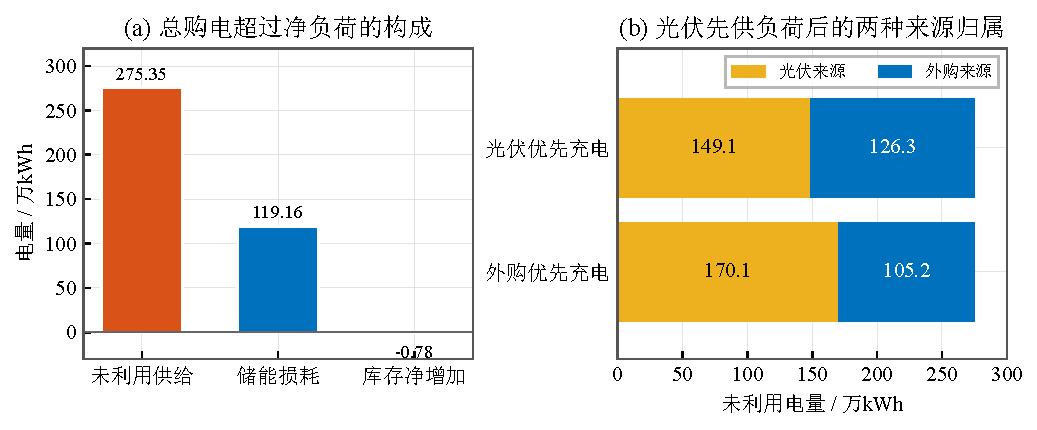
\includegraphics[width=.90\textwidth]{figures/unused_energy.pdf}
\caption{问题2多购电量由弃电、损耗和库存变化解释，弃电来源取决于分配约定}\label{fig:unused_energy}\end{figure}

\begin{figure}[htbp]\centering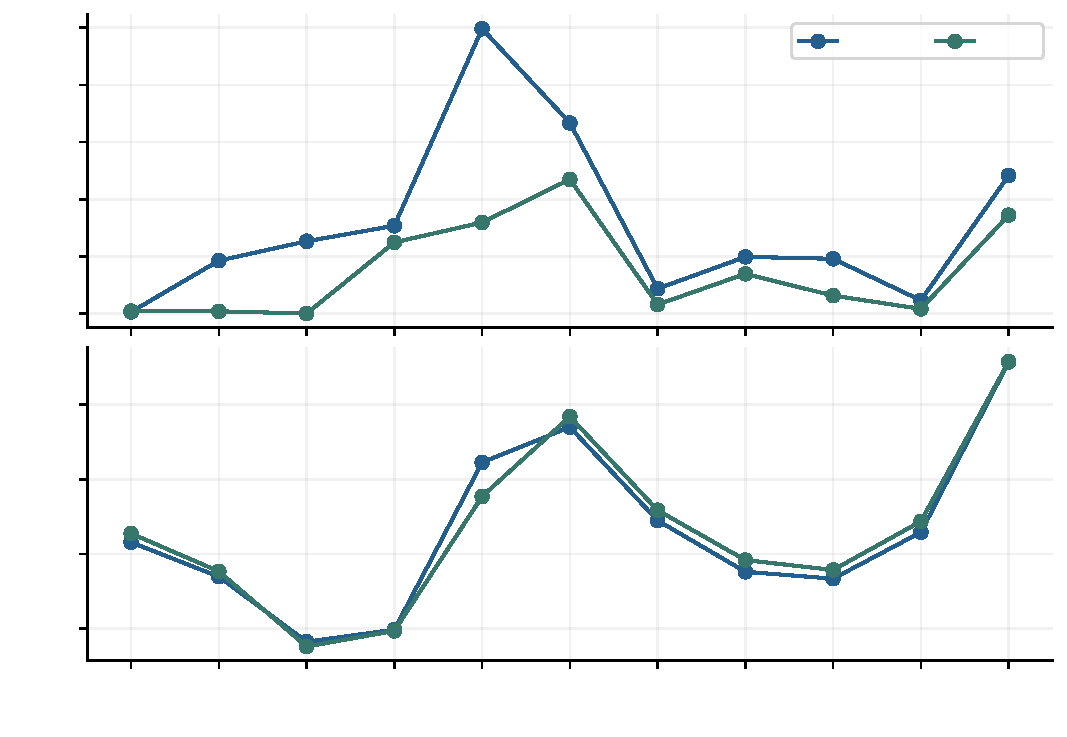
\includegraphics[width=.85\textwidth]{figures/monthly_comparison.pdf}\caption{问题2的紧急电量在6月最高，总费用峰值却出现在12月}\label{fig:monthly}\end{figure}
问题2的6月紧急购电约24.9 MWh，为各月最高；总费用最高的却是12月，约171万元。图\ref{fig:monthly}把这两个指标分开后可以看出，紧急量较少的月份仍可能因常规购电需求较大而更昂贵。


\begin{figure}[htbp]\centering
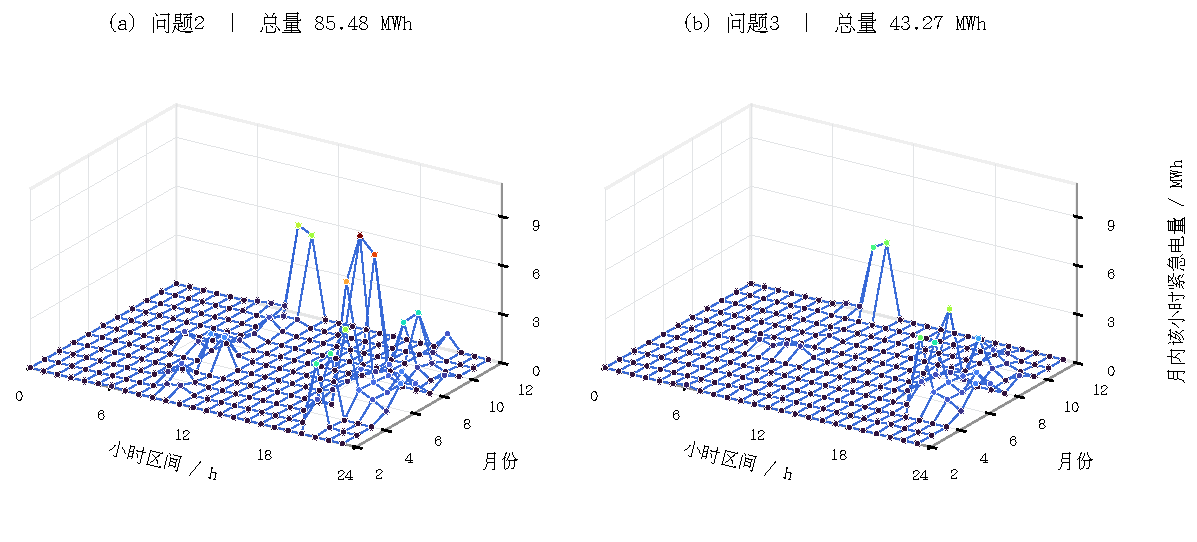
\includegraphics[width=.90\textwidth]{figures/emergency_heatmap.pdf}
\caption{问题2与问题3紧急购电的月内小时分布（三维网格，竖轴为当月该小时合计电量，两面板共用同一竖轴尺度）}\label{fig:emergency_heatmap}
\end{figure}

图\ref{fig:emergency_heatmap}把报告期的紧急购电按月、小时汇总，面板中同时标出报告期总量：问题2为85.48 MWh，问题3为43.27 MWh。两问的紧急补电都集中在少数月份的晚间时段，其余时段接近零；问题3的峰值低于问题2，但月度之内仍有局部缺额，年度紧急量下降不代表每天每个时段都改善。两套方案在零时信息和交易规则上都有差别，更新频率的净作用留到问题3的对照里单独衡量。

\subsubsection{计划保守程度与实际费用的权衡}
把式\eqref{eq:q2obj}中场景缺额的计划权重暂记为\(\rho\)，仅在独立试验中取2、3、5、8；实际紧急购电仍按题目要求的5倍电价结算。四组试验共享问题2在2月1日的实际初值及历史预测，逐日连续运行。\(\rho=5\)的重算轨迹与主结果逐项一致。

图\ref{fig:risk_tradeoff}中，权重提高使紧急量下降，未利用供给上升：由5提高到8时，紧急电量由8.55万降至4.37万kWh，但总费用增加约21.73万元；降到2时总费约1481.29万元，同样更高。四个离散试验中原权重5费用最低，我们据此不声称它在所有权重上都最优。完整数据见附录D表\ref{tab:review_risk}。

\begin{figure}[htbp]\centering
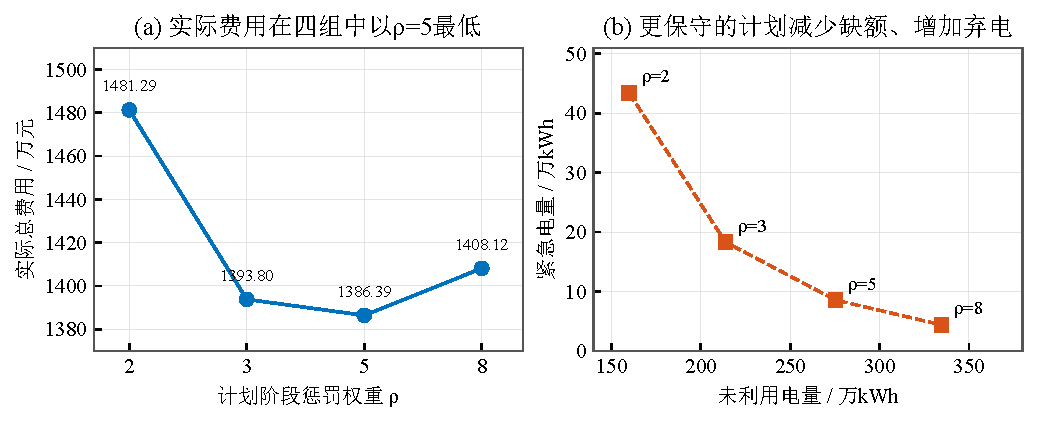
\includegraphics[width=.90\textwidth]{figures/risk_tradeoff.pdf}
\caption{实际结算倍率固定为5：更强风险预留减少紧急电，却未持续降低总费}\label{fig:risk_tradeoff}\end{figure}

\section{问题3的模型建立与求解}
\subsection{模型建立}
\subsubsection{合同基准与分段结算}
令\(P_{\mathrm{grid},d,t}^{0}\)为零时计划，\(P_{\mathrm{grid},d,t}^{(k)}\)为发布时刻\(k\)得到的调整方案，引入
\begin{equation}\label{eq:deviation}
P_{\mathrm{grid},d,t}^{(k)}-P_{\mathrm{grid},d,t}^{0}=y_{d,t}^{+}-y_{d,t}^{-},\quad y_{d,t}^{+},y_{d,t}^{-}\ge0.
\end{equation}

主口径B分别核算原计划内的履行量、取消量和新增量：履行量按原价，取消量按原价的50\%付违约费，新增量按1.5倍原价购入。原计划电量记为\(q_0\)，正式调整后的常规电量记为\(q\)，则
\begin{equation}\label{eq:piecewise}
c(q;q_0)=\begin{cases}
\lambda_tq+0.5\lambda_t(q_0-q),&0\le q\le q_0,\\
\lambda_tq_0+1.5\lambda_t(q-q_0),&q>q_0.
\end{cases}
\end{equation}

取消部分的50\%电价由第一行直接体现。用功率偏差变量整理，可得
\begin{equation}\label{eq:settleB}
C_d^{B}=\sum_t\lambda_t\left(P_{\mathrm{grid},d,t}^{0}+1.5y_{d,t}^{+}-0.5y_{d,t}^{-}+5P_{\mathrm{em},d,t}\right)\dd.
\end{equation}

下调项的负号来自“退回100\%原费、再收50\%违约费”两步合并，并非负的违约单价。例如单价1元/kWh时，原计划5 kWh正式下调至4 kWh，应付\(4+0.5\times1=4.5\)元；上调至6 kWh，应付\(5+1.5\times1=6.5\)元。若只是实际需求减少而未正式调整合同，则不产生退费。

作为原文字面解释的对照，口径A保留原计划全额电费，再收取下调违约费：
\begin{equation}\label{eq:settleA}
C_d^{A}=\sum_t\lambda_t\left(P_{\mathrm{grid},d,t}^{0}+1.5y_{d,t}^{+}+0.5y_{d,t}^{-}+5P_{\mathrm{em},d,t}\right)\dd.
\end{equation}

按口径A，5 kWh下调到4 kWh需付5.5元。允许免费处理盈余时，不下调而保留原购电始终不更差，下调不会改善目标。我们更倾向于口径B：它让取消部分的50\%价格直接发挥作用，也保留了双向调整的经济意义；口径A仍列为解释敏感性对照。
\begin{figure}[htbp]\centering
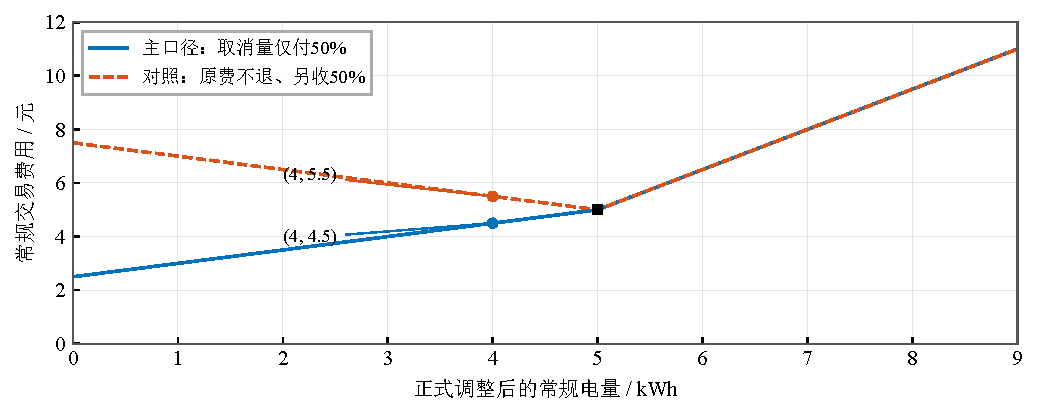
\includegraphics[width=.90\textwidth]{figures/settlement_curve.pdf}
\caption{同一原计划下两种结算解释的费用曲线（5 kWh，1元/kWh，不含紧急费）}\label{fig:settlement_curve}
\end{figure}

\subsubsection{预报更新与滚动目标}
问题3在发布时刻\(k\)读取相应预报行：发布时刻的观测记为第0个节点，其后24个整点预报为第1至24个节点，剩余10分钟区间按末端线性插值。各发布时刻分别构造误差历史——18时发布的数据绝不会出现在12时的决策里。负载预测仍在零时生成，日内不使用未来实际负载。

\begin{figure}[htbp]\centering
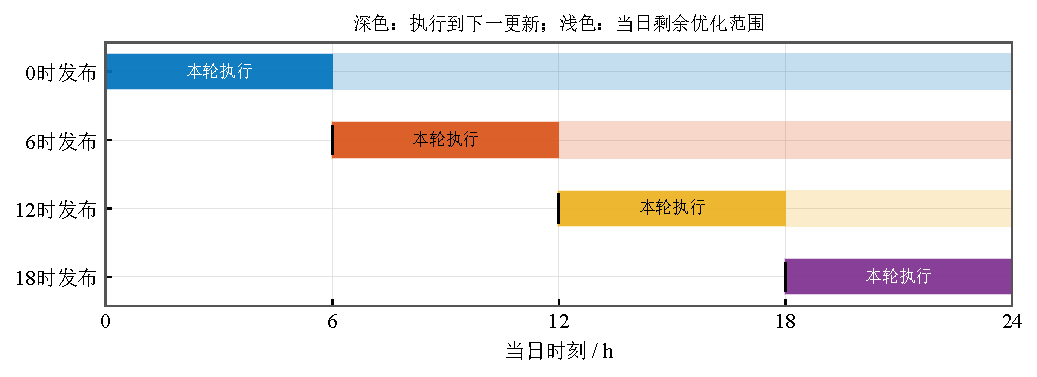
\includegraphics[width=.90\textwidth]{figures/information_timeline.pdf}
\caption{预报发布时间、剩余优化范围与本轮执行区间}\label{fig:information_timeline}
\end{figure}

零时用对应光伏预报与历史负载预测求解日前模型。对\(k=6,12,18\)，令剩余时段集合为\(\mathcal T_k=\{6k+1,\ldots,144\}\)。零时原计划一经形成就固定为结算基准，日内只更新尚未执行的安排，已执行时段不回改；原计划费在当前优化中是常数，可从目标中略去。主口径的剩余目标为
\begin{equation}\label{eq:mpc}
\min J_{d,k}=\sum_{t\in\mathcal T_k}\lambda_t(1.5y_{d,t}^{+}-0.5y_{d,t}^{-})\dd
+\frac1S\sum_s\sum_{t\in\mathcal T_k}5\lambda_tu_{d,t,s}\dd.
\end{equation}

约束包括式\eqref{eq:deviation}、更新场景下的式\eqref{eq:scenarioineq}、储能动态及功率容量边界，初始状态为发布时刻的实际电量。对照口径A把目标中的\(-0.5y^-\)换为\(+0.5y^-\)。对于主口径，同时减少等量\(y^+\)与\(y^-\)可降低目标且保持净偏差不变，因此正电价下最优解不会同时取正，无需额外二元变量，该分段线性费用可直接通过偏差变量构成LP。

本策略是有限日内剩余时域的滚动优化，遵循“更新状态、优化未来、只实施前一段”的控制思想\cite{mpc}，每轮按以下步骤执行：
\begin{center}\small
\begin{tabular}{@{}p{0.95\textwidth}@{}}
\toprule
\textbf{算法1\quad 光伏预报到达后的滚动调整与费用门控}\\
\midrule
\textbf{输入：}当前实际储电量\(E^{\mathrm{act}}_{d,0}\)，零时计划\(p^0\)，现行安排\(g^{\mathrm{keep}}\)，最新发布的光伏预报，历史误差轨迹，价格估计\(\widehat\lambda_{d,t}\)\\
\textbf{输出：}本时段执行的购电与充放电功率、更新后的安排\(g^{\mathrm{next}}\)、合同偏差结算\\
\textbf{Step 1}\quad 零时获取当前SOC、历史负载预测与零时光伏预报，形成原始全天购电计划\(p^0\)，按反馈规则执行至下一发布时刻；\\
\textbf{Step 2}\quad 读取刚发布的预报并对当日剩余时段插值，按同一发布时刻的历史误差重建场景\(n^{(k)}_{d,t,s}\)；\\
\textbf{Step 3}\quad 保持\(p^0\)不变，求解式\eqref{eq:mpc}得到剩余时段的候选安排\(g^*\)；\\
\textbf{Step 4}\quad 用同一组情景、同一当前SOC与同一价格估计，按式\eqref{eq:gate_value}比较\(\widehat V_k(g^{\mathrm{keep}})\)与\(\widehat V_k(g^*)\)，按式\eqref{eq:gate}决定采纳或保留；\\
\textbf{Step 5}\quad 只实施到下一发布时刻，按反馈规则更新实际充放电、紧急量与储电量，返回Step 2；\\
\textbf{Step 6}\quad 日末按最终生效购电量相对\(p^0\)的偏差结算一次费用，并传递实际SOC。\\
\bottomrule
\end{tabular}
\end{center}

附件预报覆盖未来24小时，本滚动基准只优化当日剩余时段，跨日部分未进入目标；终端价值在日前模型中单独检验。

\subsubsection{计入调整费的采纳规则}
预报更新并不必然触发购电调整。我们保存零时原计划\(p^0\)作为整日合同基准，另保存当前仍有效的执行安排\(g^{\mathrm{keep}}\)（可能来自上一轮已采纳的调整）。新预报到达后，式\eqref{eq:mpc}生成候选\(g^*\)；对这两条安排用同一组最新误差场景、同一当前实际SOC和同一价格估计，按式\eqref{eq:chargefeedback}--\eqref{eq:emfeedback}逐时模拟实际反馈，定义
\begin{equation}\label{eq:gate_value}
\widehat V_k(g)=\sum_{t\in\mathcal T_k}c(g_t\dd;p_t^0\dd)
+\frac1S\sum_s\sum_{t\in\mathcal T_k}5\widehat\lambda_{d,t}
P_{\mathrm{em},t,s}^{\mathrm{fb}}(g)\dd.
\end{equation}

\(c\)按式\eqref{eq:piecewise}及当时可用价格计算。紧急量\(P_{\mathrm{em}}^{\mathrm{fb}}\)由场景内连续反馈产生，与LP的共同储能轨迹不同，评分因此会受到误差发生先后次序的影响。采纳规则为
\begin{equation}\label{eq:gate}
g^{\mathrm{next}}=\begin{cases}
g^*,&\widehat V_k(g^{\mathrm{keep}})-\widehat V_k(g^*)>\epsilon,\\
g^{\mathrm{keep}},&\text{其他情形},
\end{cases}\qquad \epsilon=10^{-6}\text{元}.
\end{equation}

\(\epsilon\)只是数值容差，不是额外的固定调整费；候选评分本身已含剩余偏差费用，不会重复计费。未通过筛选时保留现行安排，原始合同\(p^0\)不变。

评分增加\(O(Sm)\)计算量，无需新增整数变量。它判断的是预测场景中的得失，实际运行仍可能出现相反结果。

\begin{figure}[htbp]\centering
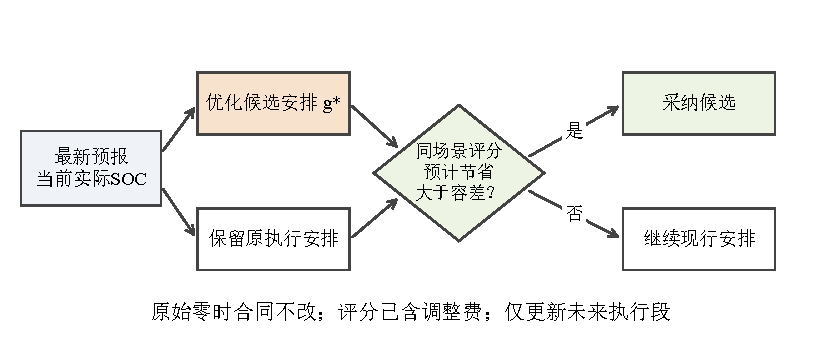
\includegraphics[width=.90\textwidth]{figures/gate_flow.pdf}
\caption{以同一信息比较候选与现行安排的日内调整采纳流程}\label{fig:gate_flow}
\end{figure}

\subsection{模型求解与结果分析}
\subsubsection{典型日的购电与操作区间}
典型日汇总见表\ref{tab:q3_daily_summary}，完整指定格式表与紧急事件见附录C。其中“调整后”表示最终生效的常规购电总量，并非相对原计划的差值。
\begin{table}[H]
\centering\small
\caption{问题3典型日购电与费用汇总}
\label{tab:q3_daily_summary}
\begin{tabular}{lrrrr}\toprule
日期 & 原计划/kWh & 调整后/kWh & 紧急/kWh & 总费用/元 \\\midrule
03-20 & 71993.11 & 66853.81 & 113.04 & 43037.70 \\
06-21 & 35054.77 & 34929.74 & 0.00 & 20690.52 \\
09-23 & 72432.47 & 67541.88 & 464.02 & 46227.25 \\
12-21 & 99503.29 & 97280.92 & 0.00 & 63388.89 \\
\bottomrule\end{tabular}
\end{table}


\begin{table}[H]
\centering\small
\caption{问题3 2025年3月20日指定时段计划与调整对照（kWh）}
\label{tab:q3_plan_adjust}
\begin{tabular}{lrrr}\toprule
时段 & 零时计划 & 最终生效 & 差额 \\\midrule
10:00--10:10 & 0.00 & 0.00 & 0.00 \\
12:00--12:10 & 674.37 & 558.17 & -116.21 \\
14:00--14:10 & 0.00 & 0.00 & 0.00 \\
16:00--16:10 & 680.86 & 537.66 & -143.20 \\
18:00--18:10 & 701.05 & 701.05 & 0.00 \\
20:00--20:10 & 0.00 & 0.00 & 0.00 \\
\bottomrule\end{tabular}
\end{table}


3月20日约7.20万kWh原计划经调整后变为约6.69万kWh。减少量主要来自下调：上调仅约13 kWh，下调约5153 kWh；相应上调费约15元、下调净退费约1772元。该日仍有约113 kWh紧急补电。

上、下调量先分时段计算再汇总费用，全天净减少量不直接套用下调费率。

9月23日，问题3紧急购电约464 kWh、总费约4.62万元；问题2约1095 kWh、4.94万元。不过两者的零时预报来源和交易规则都不一样，这笔差额不能全记在预报次数上，下节另设相同零时预报的频率对照来单独识别。
\begin{figure}[htbp]\centering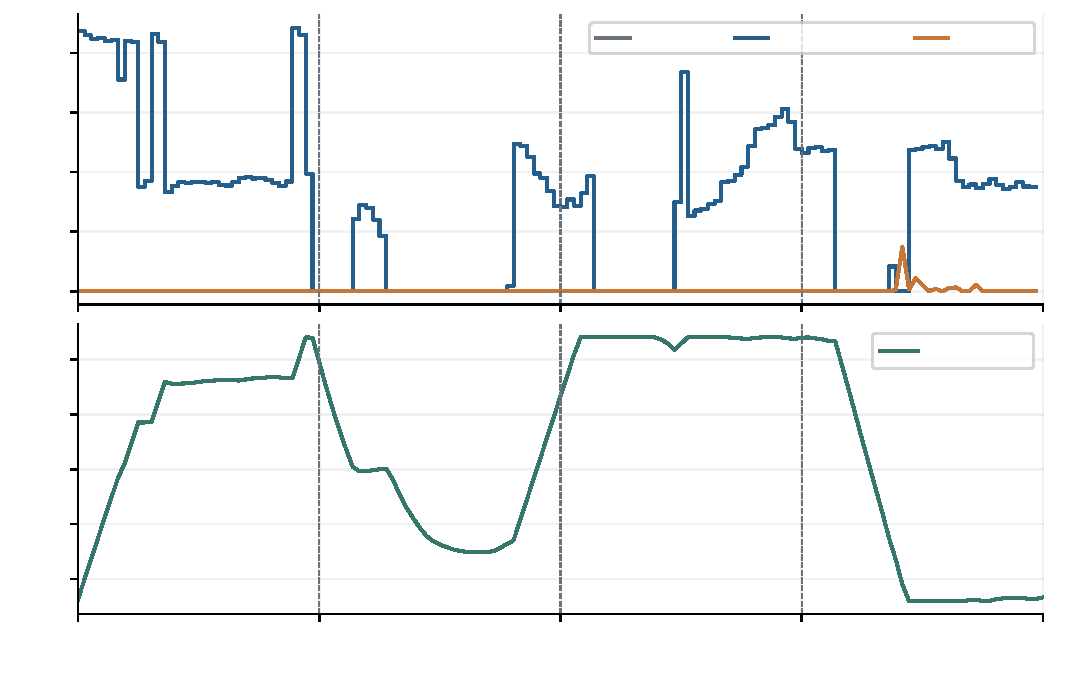
\includegraphics[width=.85\textwidth]{figures/q3_typical.pdf}\caption{3月20日多时段下调购电后仍需紧急补电；虚线标出预报更新时刻}\label{fig:q3}\end{figure}

\subsubsection{预报更新频率的经济价值}
为了单独识别日内更新的作用，使用相同零时预报、相同历史误差窗口和同一结算口径，比较仅零时决策、增加12时更新、使用全部四次预报三种方案。各方案均连续运行全年，实际SOC允许随其执行结果变化。
\begin{table}[H]
\centering\small
\caption{相同零时预报下，四次更新的报告期费用最低}
\label{tab:frequency}
\begin{tabular}{lrrrr}\toprule
预报时刻 & 上调费/元 & 下调净费/元 & 紧急电量/kWh & 总费用/元 \\\midrule
仅0时 & 0.00 & 0.00 & 77341.11 & 14010355.00 \\
0、12时 & 90237.60 & -240050.46 & 60126.17 & 13739488.19 \\
0、6、12、18时 & 164969.36 & -310478.47 & 43270.28 & 13642862.05 \\
\bottomrule\end{tabular}
\end{table}


四次更新相对仅零时决策节省约36.75万元（2.62\%），紧急电量由约7.73万kWh降至4.33万kWh。相对只在12时增加一次更新，使用6时与18时预报还少支出约9.66万元。

在附件预报不另收费、结算规则取我们主口径时，这组结果支持日内更新。若预报服务或交易另有费用，需从实际节省中扣除，不能直接沿用本次收益判断。

问题3总费约1364.29万元，比问题2低约22.10万元。但这一差额混入了零时预报来源与结算口径的变化，并非全是日内更新的收益：换用“原计划照付、另计50\%”的口径后，问题3为1393.45万元，反而比问题2高约7.06万元。日内更新的净贡献应以下节同一零时预报下的频率对照为准。费用分解方面，原计划费约1356.44万元，上调费约16.50万元，下调净退费约31.05万元，紧急费约22.40万元；下调净退费为负只是“退全费再罚一半”合并后的结果，该项已含在总费内。

附件3的零时预报并非在每个指标上都更好。其全天MAE约197 kW，高于历史预测的153 kW；但6时、12时更新对各自后续白天时段的MAE约为185 kW和140 kW，低于对应的零时预报误差（图\ref{fig:forecast_updates}；精确值见附录D表\ref{tab:issued_forecast}）。这提供了一种解释：新增信息可能改善较关键的白天时段，即使全天误差并不占优。是否节省费用仍须看实际结算，我们因此把它交给同一零时预报下的频率对照来判断。

11个月的费用差均为正，但334天中仍有67天更新后更贵，261天更便宜，6天基本相同。5月的紧急电量也有增加。

按月度费用差计算，月均节省\(\rv{editorial}{monthly_mean_wan}\pm\rv{editorial}{monthly_sd_wan}\)万元，范围\rv{editorial}{monthly_min_wan}--\rv{editorial}{monthly_max_wan}万元。其中\(\pm\)取11个月的样本标准差（分母为10），只刻画月间离散程度；各月长短、季节负荷与跨日库存都不同，该区间不能当作未来节省的置信区间。

\begin{figure}[htbp]\centering
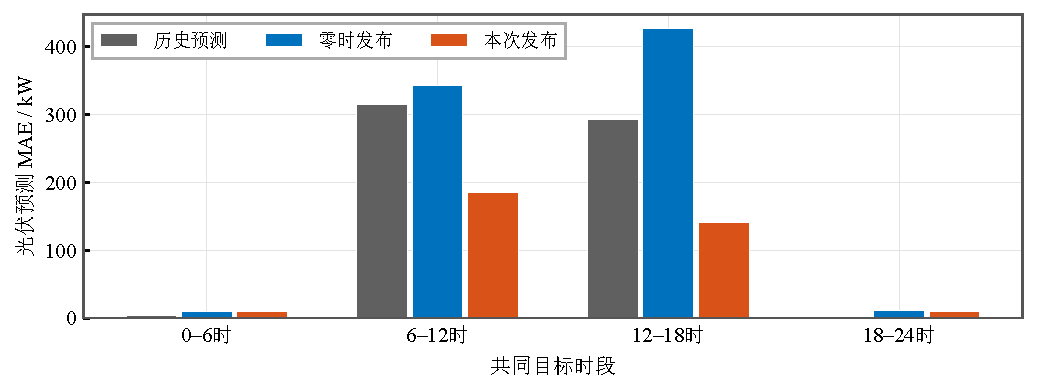
\includegraphics[width=.90\textwidth]{figures/forecast_updates.pdf}
\caption{相同目标区间内，6时和12时新预报降低了白天光伏预测MAE}\label{fig:forecast_updates}
\end{figure}

逐月费用差与紧急电量差列于附录D表\ref{tab:update_robustness}。

\begin{figure}[htbp]\centering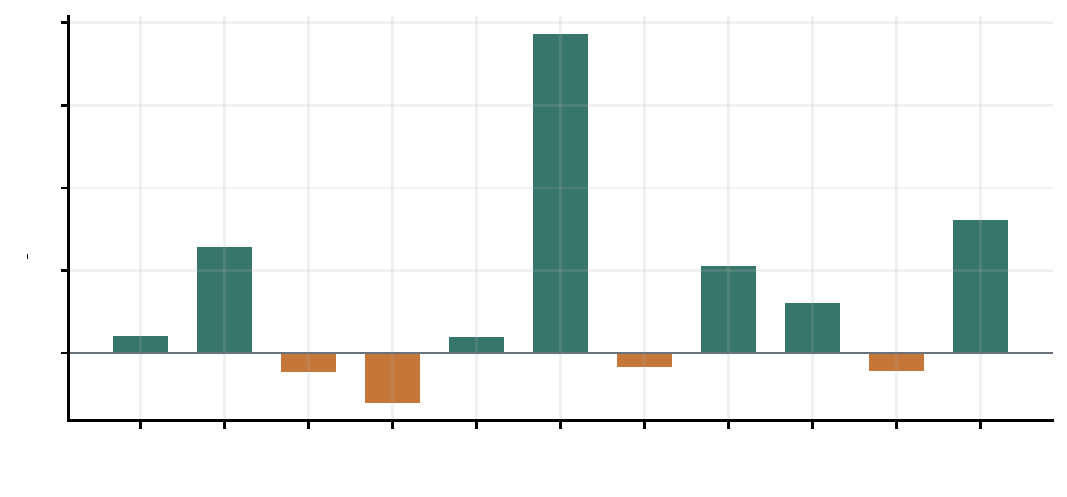
\includegraphics[width=.85\textwidth]{figures/update_robustness.pdf}\caption{四次更新在11个月均节省费用，月度幅度差异较大}\label{fig:update_robustness}\end{figure}

\subsubsection{调整采纳规则的实际收益}
\begin{table}[H]\centering\small
\caption{计费后筛选调整小幅节省总费，紧急电量略增（采纳、保留以次计）}\label{tab:gate_results}
\begin{tabular}{lrrrr}\toprule
方案 & 总费用/元 & 紧急电量/kWh & 采纳 & 保留 \\\midrule
重复价：直接滚动 & 13642862.05 & 43270.28 & 1002 & 0 \\
重复价：经济门控 & 13637232.96 & 44275.40 & 612 & 390 \\
波动价：直接滚动 & 14403672.82 & 43101.90 & 1002 & 0 \\
波动价：经济门控 & 14397071.03 & 43799.31 & 609 & 393 \\
\bottomrule\end{tabular}\end{table}


1002次日内机会中，重复电价方案采纳612次，另有119次候选预计更贵、271次预计费用基本相同。与直接滚动相比，最终节省约5629元，仅约0.04\%。波动电价下节省约6602元。收益并不大。

两种门控方案的紧急电量反而略有增加，净收益来自各项费用的共同变化；表中“直接滚动采纳1002次”指每次都采用优化解，不代表每次的购电量都真的变了。

门控与直接滚动的轨迹分别保存。五个规定工作簿仍采用直接滚动等既定主方案，便于逐项复核每个改动的效果。

\section{问题4的模型建立与求解}
附件4记录实际交易价格，却未说明何时发布。我们把未来价格未知作为主设定：历史价格预测参与计划，实际价格参与结算；当天完整价格已知的情形单列。两者都沿用前问的储能与功率约束。
\subsection{模型建立}
\subsubsection{未来价格未知的主设定}
价格未知时，把计划里用到的价格全部换成预测价\(\widehat\lambda_{d,t}\)；到了结算，再全部换回附件4的实际价\(\lambda_{d,t}\)。以问题4的滚动目标为例，替换后为
\begin{equation}\label{eq:priceobj}
\min\sum_{t\in\mathcal T_k}\widehat\lambda_{d,t}(1.5y_{d,t}^{+}-0.5y_{d,t}^{-})\dd
+\frac1S\sum_s\sum_{t\in\mathcal T_k}5\widehat\lambda_{d,t}u_{d,t,s}\dd.
\end{equation}

物理约束和偏差定义沿用前三问。价格按同星期均值预测，6、12、18时更新光伏时不更新价格预测。这里尚未构建日内价格预测器，即使更新时刻已经观测到当天此前价格，也不重估剩余价格，这一简化可能限制日内调节效果。两个问题4工作簿均使用该设定；把当天实际价格作为已公布曲线输入的情况仅出现在对照模型中。

\subsubsection{当天价格已知的对照设定}
对照模型在每天零时获知当天附件4价格曲线，令\(\widehat\lambda_{d,t}=\lambda_{d,t}\)，但未来负载与光伏实际量仍然未知。设置该方案是为了分离价格信息的影响；它不是全信息完美预测，其费用也不构成全年最优下界。

\subsection{模型求解与结果分析}
\subsubsection{价格信息与储能循环}
\begin{table}[H]
\centering\small
\caption{提前获知价格降低回测费用，并增加储能循环强度}
\label{tab:price_information}
\begin{tabular}{lrrrr}\toprule
模型与信息 & 计划费/万元 & 紧急电量/kWh & 总费用/万元 & 等效循环 \\\midrule
日前，价格预测 & 1410.86 & 83563.75 & 1462.14 & 591.46 \\
日前，价格已知 & 1398.32 & 86659.63 & 1451.68 & 622.10 \\
滚动，价格预测 & 1431.33 & 43101.90 & 1440.37 & 597.33 \\
滚动，价格已知 & 1418.38 & 43877.11 & 1428.33 & 627.39 \\
\bottomrule\end{tabular}
\end{table}


提前已知当天价格时，日前、滚动方案总费分别为1451.68万元、1428.33万元；相对价格预测主方案分别少支出约10.46万元、12.04万元，约为0.72\%、0.84\%。两套方案的储能等效循环分别由约591、597次增至622、627次。

更准确的价差信息增加了调节活动。我们把结论限定在交易费用层面：没有计入循环寿命成本，长期经济性尚不能据此确定。

价格预测设定继续对应\texttt{result4-2.xlsx}和\texttt{result4-3.xlsx}。价格已知的两份逐时结果以“补充\_价格已知”前缀单独提供。前者强调决策时的信息限制，后者对应把附件4直接作为已知价格参数的解读；我们把两套结果分别保存，不混填为一份答案。

\subsubsection{典型日及费用构成}
两套可实施方案的四个指定日期汇总见表\ref{tab:q4_2_daily_summary}和表\ref{tab:q4_3_daily_summary}，对应紧急事件见附录C表\ref{tab:q4_2_emergency}和表\ref{tab:q4_3_emergency}。完整的指定时段购电表和4小时充放电表列于附录C，全部334天结果写入所要求的两个工作簿。
\begin{table}[H]
\centering\small
\caption{问题4-2典型日购电与费用汇总}
\label{tab:q4_2_daily_summary}
\begin{tabular}{lrrrr}\toprule
日期 & 原计划/kWh & 调整后/kWh & 紧急/kWh & 总费用/元 \\\midrule
03-20 & 69026.66 & 69026.66 & 0.00 & 43411.08 \\
06-21 & 36837.19 & 36837.19 & 0.00 & 18609.89 \\
09-23 & 68830.77 & 68830.77 & 1076.53 & 51152.10 \\
12-21 & 98222.77 & 98222.77 & 0.00 & 74692.77 \\
\bottomrule\end{tabular}
\end{table}

\begin{table}[H]
\centering\small
\caption{问题4-3典型日购电与费用汇总}
\label{tab:q4_3_daily_summary}
\begin{tabular}{lrrrr}\toprule
日期 & 原计划/kWh & 调整后/kWh & 紧急/kWh & 总费用/元 \\\midrule
03-20 & 71871.84 & 66695.93 & 114.06 & 44535.29 \\
06-21 & 35397.64 & 35241.80 & 0.00 & 18088.21 \\
09-23 & 72586.44 & 67662.34 & 466.14 & 48346.91 \\
12-21 & 99343.17 & 97208.96 & 0.00 & 74630.49 \\
\bottomrule\end{tabular}
\end{table}


价格波动并未在每个日期都提高费用：6月21日，日前方案由重复电价下约2.15万元降至1.86万元，12月21日却由约6.35万元升至7.47万元。价格水平和价差出现的时段，与当时净负荷是否匹配，比“波动更大”这个概括更能解释差异。
\begin{figure}[htbp]\centering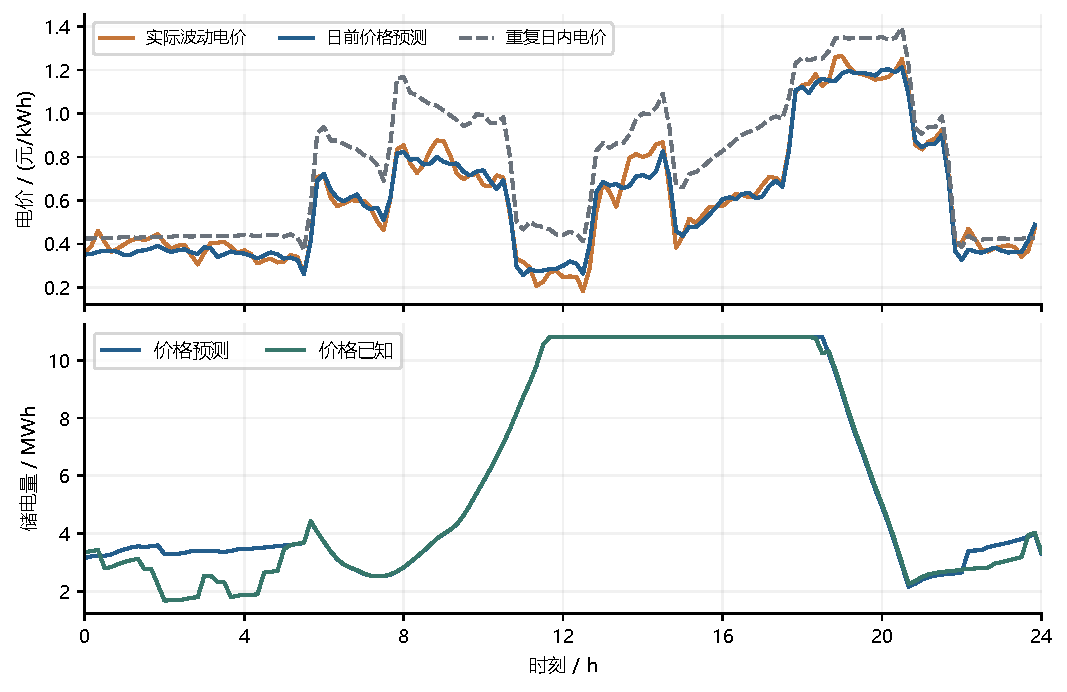
\includegraphics[width=.85\textwidth]{figures/q4_price.pdf}\caption{价格信息差异改变储能调度轨迹（6月21日）}\label{fig:q4}\end{figure}
\begin{table}[H]
\centering\small
\caption{本样本中，波动电价下两套主方案的费用均高于重复电价基准}
\label{tab:annual}
\begin{tabular}{lrrrrr}\toprule
模型 & 计划费 & 上调费 & 下调净费 & 紧急费 & 总费用 \\\midrule
问题2 & 1337.62 & 0.00 & 0.00 & 48.77 & 1386.39 \\
问题3 & 1356.44 & 16.50 & -31.05 & 22.40 & 1364.29 \\
问题4-2 & 1410.86 & 0.00 & 0.00 & 51.28 & 1462.14 \\
问题4-3 & 1431.33 & 17.81 & -33.01 & 24.24 & 1440.37 \\
\bottomrule\end{tabular}
\end{table}

\begin{figure}[htbp]\centering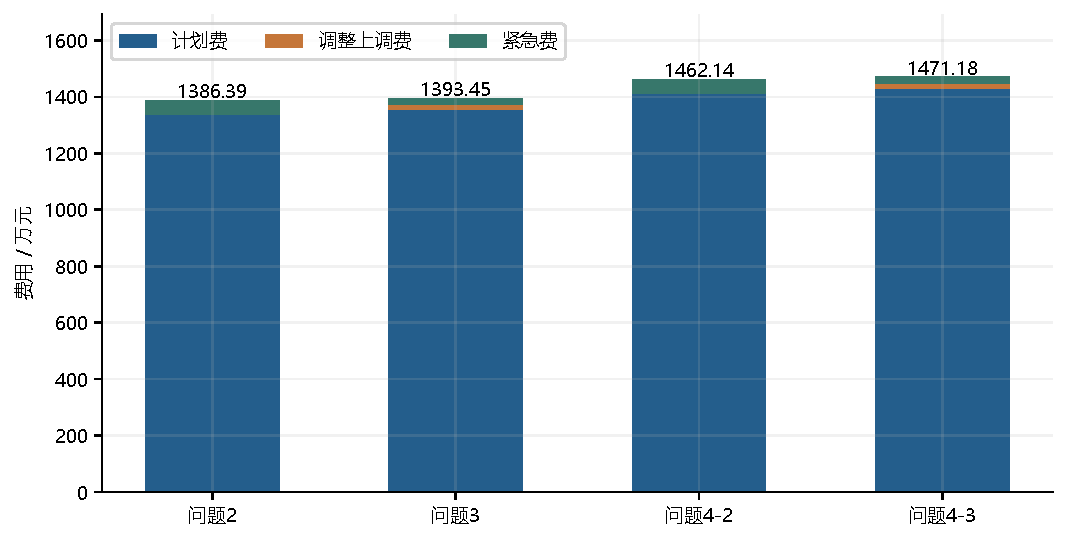
\includegraphics[width=.85\textwidth]{figures/annual_costs.pdf}\caption{本样本的波动电价方案总费更高，履行原计划费占主要部分}\label{fig:annual}\end{figure}
报告期内，波动电价两套主方案总费约1462.14万元和1440.37万元，均高于对应的重复电价基准。图\ref{fig:annual}把费用拆成履行原计划费、取消违约费、新增购电费、紧急费四个非负项，加起来恰等于表\ref{tab:annual}的总费；其中履行原计划费是\(C_0+2C_-\)、取消违约费是\(-C_-\)。注意表里\(C_-\)按负数记，两种拆法不能混着加。另外，换价格后调度轨迹本身也变了，费用差不能全部解读为价格预测损失。

\subsubsection{稀疏模型规模与计算耗时}
剩余时域为\(m\)个时段、场景数为\(S\)时，日前模型包含\((4+S)m\)个连续变量、\(m\)个状态等式与\(Sm\)个场景不等式；调整模型再增加\(2m\)个偏差变量与\(m\)个计划差等式。矩阵非零元数量和构造空间均为\(O(Sm)\)。成熟阶段\(S=15\)，全天日前模型有2736个连续变量；在6时更新时，\(m=108\)，调整模型有2268个变量。

全年逐日前模型共调用365次LP，四次预报滚动模型1460次；只计2月至12月分别为334次和1336次，其余用于1月初始化。求解时间受稀疏结构、退化性、算法选择和机器条件影响，不能由矩阵规模直接推出总运行时间也是\(O(Sm)\)。实测耗时见表\ref{tab:runtime}，其中不含依赖安装、绘图、工作簿输出与LaTeX编译。
\begin{table}[H]
\centering\small
\caption{主模型的实测运行时间（含全年初始化）}
\label{tab:runtime}
\begin{tabular}{lrrr}\toprule
模型 & LP次数 & LP耗时/s & 全年仿真/s \\\midrule
问题2 & 365 & 6.32 & 6.43 \\
问题3 & 1460 & 17.24 & 17.46 \\
问题4-2 & 365 & 5.46 & 5.55 \\
问题4-3 & 1460 & 16.87 & 17.09 \\
\bottomrule\end{tabular}
\end{table}


\section{模型检验与改进}
\subsection{物理约束、费用与信息时序核验}
核验记录显示，\rv{derived}{case_count}组主模型及对照中，实际功率平衡的最大残差不超过\(9.1\times10^{-13}\) kW，日费用复算差不超过\(5.9\times10^{-11}\)元，名义LP约束残差小于\(10^{-7}\)；SOC全程位于1200--10800 kWh，未出现实际同时充放电。这些数字说明的是计算实现与模型一致，与预测误差无关。

因果性检查把第181天之后的实际量与预报做了扰动，前180天的问题2决策逐项不变；对问题3的四个决策时刻分别扰动当时尚未发布的信息，当前解同样不变。结算规则另用5 kWh分别调到4、5、6、0 kWh的例子核对，单价1元时应付4.5、5、6.5、2.5元，与程序输出一致。工作簿保存后重新读取，与轨迹逐项核对无误。

时间配对诊断暴露了风险代理的一项局限。对9月23日的场景逐列独立打乱（随机种子20260911），LP代理目标几乎不变，实际反馈费用却改变了（表\ref{tab:scenario_diagnostic}）。原因在于LP共用储能轨迹，逐时缺额代价没有利用跨时段配对。

因此，我们只将其称为\textbf{逐时缺额风险代理}。保存了整条历史误差，并不等于优化器已经利用了误差的时间相关性。

\begin{figure}[htbp]\centering
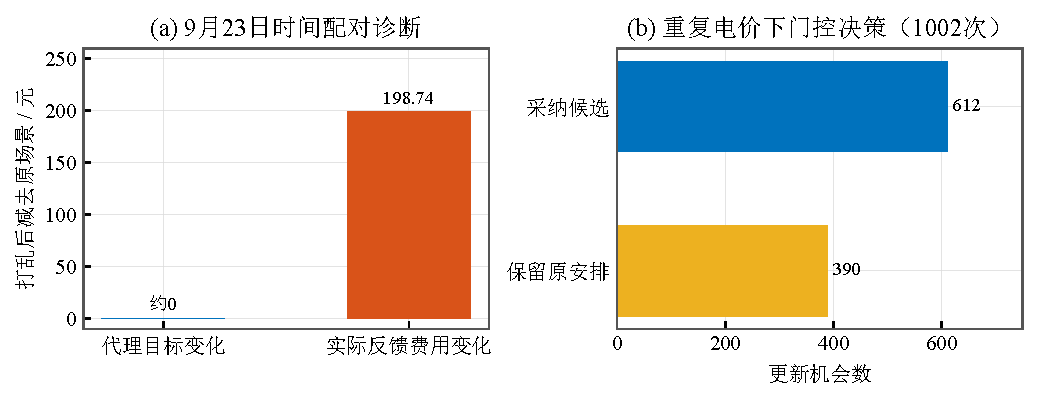
\includegraphics[width=.90\textwidth]{figures/proxy_and_gate.pdf}
\caption{代理目标与实际反馈可有不同响应，门控也会保留部分原安排}\label{fig:proxy_and_gate}\end{figure}
图\ref{fig:proxy_and_gate}(a)中，同一初值下代理目标变化约为零，实际反馈费用却增加约199元；(b)单独列出门控的采纳数量。两张图分别对应评价环节的两个侧面。

固定问题2常规购电计划后，另试验36时段储能保留规则：根据日前预测的后续缺额留电，再在容量和功率边界内放电。它使报告期总费增加约87.49万元，紧急购电增加约18万kWh；只有20天更便宜，214天更贵。

该对照未改善即时放电策略：保留规则增加了当期高价补电，却未在后续兑现足够收益，但单次对照不足以判定即时放电最优。

\subsection{结算与参数敏感性}
主模型与各项独立试验的关键参数及确定方式见表\ref{tab:key_params}：涉及信息与风险的参数均由已完成日期的验证结果选定，报告期不再调整；涉及题意歧义的参数则并列两种解释重新求解，不因某种解释结果更低而选用它。
\begin{table}[H]
\centering\small
\caption{关键参数的取值与确定方式}
\label{tab:key_params}
\begin{tabular}{>{\raggedright\arraybackslash}p{3.4cm}l>{\raggedright\arraybackslash}p{7.6cm}}\toprule
参数 & 取值 & 确定方式\\\midrule
误差回看窗口\(H\) & 14天 & 主模型事先设定，第9.2节比较7、14、28天窗口；属事后敏感性范围，不是置信区间\\
情景数\(S\) & 15 & 14条历史误差轨迹加1条零误差轨迹，等权重近似误差经验分布\\
缺额计划权重\(\rho\) & 5 & 与题面紧急购电的5倍电价一致；第6.3.4节另取2、3、5、8作保守度试验，结算始终按5倍\\
终端价值系数\(\gamma\) & 0或0.5 & 由1月15--31日验证期的库存修正费用选出，2月起冻结\\
预报融合权重\(\alpha_k\) & 0.25/0.50/0.75/0 & 由1月份各发布时刻的剩余当日光伏MAE选出，零时用整日误差评价\\
采纳容差\(\epsilon\) & \(10^{-6}\)元 & 数值容差，只用于判断候选是否严格更优，不是固定调整费\\
时间步长\(\dd\) & 1/6 h & 题目给定的10分钟调度间隔\\
充放电效率\(\eta_c,\eta_d\) & 0.9 & 题面90\%的单程解释；第5.3.3节并列回路效率等其他解释的单日费用\\
\bottomrule\end{tabular}
\end{table}
\begin{table}[H]
\centering\small
\caption{两种结算口径的敏感性比较}
\label{tab:settlement}
\begin{tabular}{lrrr}\toprule
价格条件与口径 & 下调电量/kWh & 下调净费/元 & 总费用/元 \\\midrule
重复日内价，主口径 & 0.00 & 0.00 & 13934495.57 \\
重复日内价，退费 & 1022284.79 & -310478.47 & 13642862.05 \\
波动电价，主口径 & 0.00 & 0.00 & 14711757.51 \\
波动电价，退费 & 1037194.76 & -330099.56 & 14403672.82 \\
\bottomrule\end{tabular}
\end{table}


口径B下，问题3累计下调约102万kWh，对应净退费约31.05万元；相对于原费不退且另罚的口径A，总费少约29.16万元，波动价滚动方案少约30.81万元。这里两种解释各自重新优化，费用差并非给同一轨迹简单换费率的结果。

两种口径的取舍最终取决于题意，而不是哪种算出来便宜；好在两种口径下日内更新都成立：口径A的问题3合计1393.45万元，仍比同一零时预报下不更新的1401.04万元低7.59万元（0.54\%），只是幅度远小于口径B的36.75万元。
附录D表\ref{tab:window}给出三个窗口的精确结果。

7、14、28天窗口的费用约为1348.65万、1364.29万、1373.80万元，越短的窗口在这个报告期表现越好。一种解释是较早的误差对当前分布的代表性在下降；但窗口长短也改变了跨日库存，单凭这组试验还分不清主因。

这三个值构成参数敏感性范围，不是重复实验的误差条。主窗口维持事先选定的14天；若想自适应选窗，每次决策前都只能用已完成日期验证。

不同策略在统计期边界保有的储能库存略有差异。为进行辅助比较，可取统一参考价值\(v=0.9\times0.4248\approx0.382\)元/kWh，定义库存调整费用
\begin{equation}\label{eq:inventory}
C_{\mathrm{adj}}=C_{\mathrm{total}}+vE_{32,0}-vE_{365,144}.
\end{equation}

该量仅作同一库存估值下的比较，不替代题目要求的实际现金费用。问题2报告期净消耗库存7788.15 kWh，按原参考值修正需增加约2978元，占现金费用约0.02\%。另以附件4全期价格范围乘放电效率，取统一估值\(v\in[0.007,1.614]\)元/内部kWh作事后敏感性分析，问题2修正量约为53至12572元。该范围不是决策时使用的价格信息，也不是置信区间。

在整个估值范围内，四套主模型的费用次序保持为问题3、问题2、问题4-3、问题4-2，价格已知相对预测价格的优势也没有反转。该次序仅针对这里列出的比较。
\begin{figure}[htbp]\centering
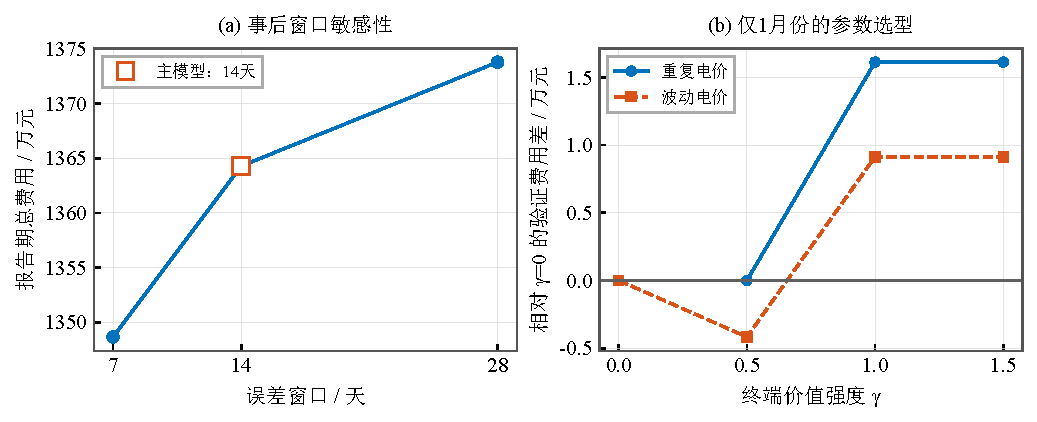
\includegraphics[width=.90\textwidth]{figures/parameter_sensitivity.pdf}
\caption{误差窗口的事后敏感性与终端价值的1月验证结果采用不同信息范围}\label{fig:parameter_sensitivity}
\end{figure}

\subsection{历史信息与发布预报融合}
发布预报在白天的优势较明显，历史预测对部分时段也有价值。我们用凸组合检验两类信息是否可以互补：
\begin{equation}\label{eq:blend}
\widehat P_{\mathrm{pv},d,t}^{(k),\mathrm{mix}}
=\alpha_k\widehat P_{\mathrm{pv},d,t}^{(k)}+(1-\alpha_k)\widehat P_{\mathrm{pv},d,t}^{\mathrm{hist}}.
\end{equation}

对每个发布时刻，\(\alpha_k\)从\(\{0,0.25,0.5,0.75,1\}\)中按1月15--31日剩余当日光伏预测的MAE选定，2月起固定，不用报告期费用反选权重。零时的权重按全天误差来评，免得夜间误差占了大头、选出不合适的白天权重。1月照旧用原发布预报热启动，融合从2月才开始用；算误差场景时，用各阶段实际采用的那套预测。
\begin{table}[H]
\centering\small
\caption{仅由1月15--31日剩余当日MAE确定的发布预报权重}
\label{tab:blend_weights}
\begin{tabular}{lrrr}\toprule
发布时间 & 发布预报权重 & 历史预测权重 & 验证MAE/kW \\\midrule
0时 & 0.25 & 0.75 & 78.59 \\
6时 & 0.50 & 0.50 & 102.31 \\
12时 & 0.75 & 0.25 & 47.89 \\
18时 & 0.00 & 1.00 & 0.00 \\
\bottomrule\end{tabular}
\end{table}

\begin{table}[H]
\centering\small
\caption{预报融合降低了总费，但紧急电量并未同步下降}
\label{tab:blend_results}
\begin{tabular}{lrrrr}\toprule
价格与预报 & 计划费/万元 & 调整净费/万元 & 紧急量/kWh & 总费用/万元 \\\midrule
重复价，发布预报 & 1356.44 & -14.55 & 43270.28 & 1364.29 \\
重复价，融合预报 & 1329.23 & -6.89 & 46172.34 & 1346.17 \\
波动价，发布预报 & 1431.33 & -15.20 & 43101.90 & 1440.37 \\
波动价，融合预报 & 1402.47 & -6.78 & 44752.90 & 1420.75 \\
\bottomrule\end{tabular}
\end{table}


融合方案在重复电价和波动电价下分别少支出约18.11万元、19.62万元，降幅约1.33\%、1.36\%。但重复电价下的紧急电量由约4.33万kWh升到4.62万kWh。总费下降与紧急量上升可以同时发生，选预测器时两个指标都得看。

融合结果单独报告，规定工作簿仍对应原发布预报主模型；一年的样本外结果尚不足以确认权重的跨年度稳定性。

\subsection{费用驱动的预测选型}
相同大小的预测误差，发生在不同价格和SOC条件下，费用代价可以相差很大。为检验误差选型是否合适，我们固定负荷预测、窗口和执行规则，仅更换光伏候选方法，按1月15--31日的实际费用选型，并以统一价格校正期末库存。
两类指标在1月份的候选得分见附录D表\ref{tab:economic_validation}。

两种价格条件下，费用选型均选择3日均值，而MAE选型选择7日均值。候选在1月份逐日只使用之前的观测；选型完成后固定方法，报告期仅滚动更新历史输入。为隔离“选型指标”本身，MAE对照同样使用全部候选的历史预测回放；两套策略共享原主模型1月末的实际SOC，其他物理约束、场景窗口与结算规则一致。
\begin{table}[H]\centering\small
\caption{相同历史回放下，费用选型未优于MAE选型（2--12月）}\label{tab:economic_results}
\begin{tabular}{lrrr}\toprule
选择规则 & 光伏方法 & 总费用/元 & 紧急电量/kWh \\\midrule
重复价：MAE选型 & 7日均值 & 13852291.37 & 85480.79 \\
重复价：费用选型 & 3日均值 & 13858729.92 & 80511.05 \\
波动价：MAE选型 & 7日均值 & 14608269.34 & 83582.10 \\
波动价：费用选型 & 3日均值 & 14614183.70 & 78832.98 \\
\bottomrule\end{tabular}\end{table}


结果与预期并不一致。1月份费用较低的3日均值，在报告期反而比同口径MAE选型多支出约6439元和5914元（分别对应两种价格）。短验证期的费用最优没有延续到全年，我们据此保留原主预测方案，不再用报告期挑选另一个赢家。

比较须使用表中的专设MAE对照：其历史回放从1月15日开始，与原主模型1月份的持久性预测缓存不同，直接对比会把缓存差异混入选型效果。

主模型与对照共27组年度配置，新增的12组轨迹均通过物理、费用与决策时序检查。各项改动的节省不可相加：终端价值、门控、费用选型与融合还没有做过组合验证。
\begin{figure}[htbp]\centering
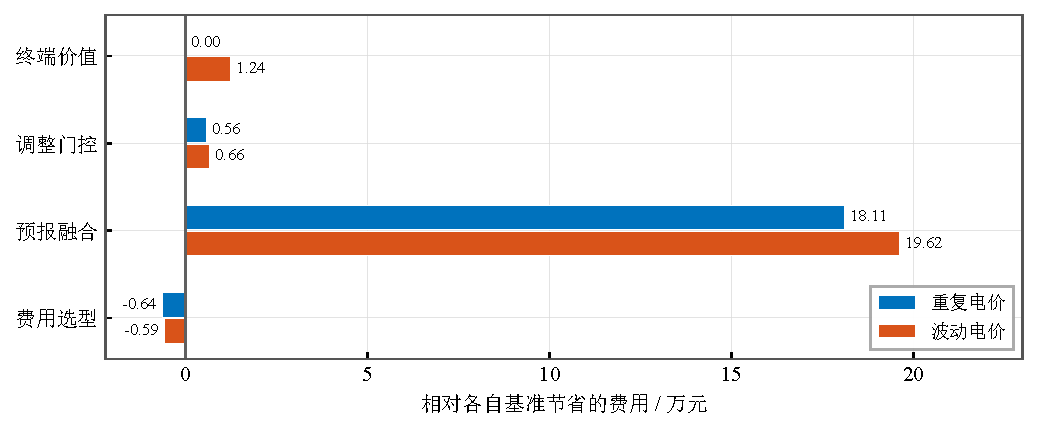
\includegraphics[width=.78\textwidth]{figures/strategy_gains.pdf}
\caption{独立改动相对各自基准的费用变化：费用选型未获改善，各项收益不可相加}\label{fig:strategy_gains}
\end{figure}

\section{模型评价与推广}
\subsection{主要创新点}
我们在建模、算法与评价三个层面都有区别于常规做法的处理。（1）建模层面，用共同名义储能轨迹加情景缺额变量构成线性风险代理，把缺额的期望代价写成目标函数中的线性项，带不确定性的全年回测因此仍可用稀疏LP求解，不必引入场景相关的储能状态与整数变量。（2）算法层面，给出保持储能状态与费用不变的同成本等价变换，证明主模型参数下总存在不同时充放电的最优解；同时以分段线性函数表达合同的三段结算，滚动调整问题保持线性。（3）评价层面，所有改进都以同信息、同物理约束、同结算口径的基准对照呈现，把信息价值、算法收益与结算口径的影响分开计量；对代理目标与执行反馈的不一致还给出定量上界，而不是笼统断言模型有效。
\subsection{主要结论}
（1）储能和日内预报更新都能降低电费，但幅度有限，也不是每个时段都成立：储能使问题1单日电费下降26.90\%；问题3的四次日内更新使全年费用降低36.75万元（2.62\%），334天里仍有67天更新后更贵；是否采纳某次更新要看评分，1002次机会采纳了612次。

（2）结论依赖结算口径与信息条件：取消费用改按“原费不退、另罚50\%”解释时，日内更新的节省从36.75万元缩到7.59万元，方向不变；当天价格从未知变为已知，全年费用也只再降0.72\%--0.84\%。结算规则或信息发布时点一变，策略就要重算。

（3）预测误差更小、紧急电量更少，都不等于总费用更低：融合试验里紧急电量上升而总费下降，费用选型里验证期更优的方法全年反而更贵。我们因此同时看误差指标与实际费用，不以单一指标替代调控目标。

\subsection{模型优点}
（1）四问共用同一套功率、能量与交易口径，每次只改动信息条件或交易规则中的一项，费用变化能明确归因；可实施策略、当日先知、全期先知三种信息水平分开建模，节省不与信息优势混记。稀疏LP使全年逐日回测可行，轨迹可逐时复核。

（2）把缺额按5倍电价补购的代价提前写进目标函数，让计划为预测误差留出余量：与点预测基准相比，问题2净节省约213万元，紧急电量由约67.4万kWh降到8.55万kWh，是各问中收益最大的一处设计。

（3）对容易歧义之处都做了对照计算：取消费用的两种解释、充放电效率的三种分配、风险权重与误差窗口敏感性、价格信息的两种可见性设定。主要结论在多种解释下方向一致，各表数字可复核、可复算。

\subsection{模型不足}
（1）场景缺额用一条共同的名义储能轨迹近似，实际电池却按观测反馈运行，代理目标与真实费用之间有系统差。以当日完全预知的执行为参照上界，报告期现金费用可由\rv{review}{oraclebase_wan}万元进一步降到\rv{review}{oracleoracle_wan}万元，相差\rv{review}{oraclecash_saving_wan}万元（约\rv{review}{oraclepercent}\%，见附录D表\ref{tab:review_oracle}）；差距不算大，但代理结构仍有改进空间，门控也保证不了真实天气下同样划算。

（2）电池循环寿命、温度与效率变化未进入模型，价格已知时等效循环升至627次，长期经济性无法判断；问题2常规购电峰值约10203 kW，高于负荷峰值约7979 kW，若实际并网容量受限，高负荷时段的方案需要重排。

（3）波动电价主方案没有日内价格预测器，日内调节因此受限；验证数据只有一年，终端奖励、短期费用选型、36时段保留规则在本数据集上都没有收益，分不清是确实无效还是仅在本样本无效。

\subsection{改进与推广}
（1）先校正风险代理，再扩展时域：引入分场景储能状态与非预见性约束\cite{stochastic}，检验代理目标与实际反馈费用的差距能否缩小，再把决策时域扩展到24--48小时，考察线性终端价值能替代多少跨日决策\cite{bertsekas}。

（2）获得电池循环寿命与温度资料后，把折旧成本计入目标，重新评价价格已知设定、融合方案等调节频繁策略的长期收益。

（3）方法与窗口按时间顺序、只用已完成日期重新验证，保留未参与选型的测试期；证据补齐之前，我们的结果适合作为可复核的调度基准，而不宜直接当作长期收益的承诺。

\section*{AI工具使用声明}
本参赛队在竞赛过程中使用了AI工具，主要用于模型讨论、代码生成与调试、数据核验、绘图及文字结构调整，详见支撑材料《AI工具使用详情》。我们把辅助范围限定在上述环节，所有由AI参与的输出都在写入论文前经我们逐项人工复核；该文件中的每条数值主张，我们都能回溯到工作簿或结果数组。

\section{参考文献}
我们的引用取自方法的原始文献、官方文档与所用求解器的正式出处，正文相应位置都给出了标注。我们只保留与建模、求解和检验直接相关的条目；凡是我们没有实际使用的方法，不列入凑数。
\begingroup
\renewcommand{\refname}{参考文献}
\begin{thebibliography}{9}\footnotesize\setlength{\itemsep}{0pt}\linespread{0.93}\selectfont
\bibitem{boyd} Boyd S, Vandenberghe L. Convex Optimization[M]. Cambridge: Cambridge University Press, 2004.
\bibitem{scipy} SciPy Developers. scipy.optimize.linprog: Linear programming[EB/OL]. [2026-09-10]. \url{https://docs.scipy.org/doc/scipy/reference/generated/scipy.optimize.linprog.html}.
\bibitem{highs} Huangfu Q, Hall J A J. Parallelizing the dual revised simplex method[J]. Mathematical Programming Computation, 2018, 10(1):119--142. DOI:10.1007/s12532-017-0130-5.
\bibitem{forecast} Hyndman R J, Athanasopoulos G. Forecasting: Principles and Practice[M/OL]. 3rd ed. Melbourne: OTexts, 2021. [2026-09-10]. \url{https://otexts.com/fpp3/}.
\bibitem{birge} Birge J R, Louveaux F. Introduction to Stochastic Programming[M]. 2nd ed. New York: Springer, 2011. DOI:10.1007/978-1-4614-0237-4.
\bibitem{mpc} Rawlings J B, Mayne D Q, Diehl M M. Model Predictive Control: Theory, Computation, and Design[M]. 2nd ed. Nob Hill Publishing, 2017.
\bibitem{stochastic} Shapiro A, Dentcheva D, Ruszczynski A. Lectures on Stochastic Programming: Modeling and Theory[M]. 3rd ed. Philadelphia: SIAM, 2021. DOI:10.1137/1.9781611976595.
\bibitem{bertsekas} Bertsekas D P. Dynamic Programming and Optimal Control, Volume I[M]. 4th ed. Nashua: Athena Scientific, 2017.
\end{thebibliography}
\endgroup
\clearpage
\section*{附录A\quad 支撑材料与程序实现说明}
\subsection*{A.1\quad 运行环境与文件组织}
计算结果来自所附程序的运行记录，环境为Python 3.12.14、NumPy 2.5.3、SciPy 1.18.1，openpyxl处理结果模板，Matplotlib绘图，XeLaTeX编译。论文保留27组主模型与对照结果，另用独立LP复算问题1，并补充效率与风险权重试验。

绘图程序读取核对后的轨迹，生成18个论文图组及源数据清单；补充程序生成复核数据和4个新图组；\texttt{verify\_consistency.py}只读取已有工作簿、表格与结果数组，重算论文数字与工作簿的对应关系，不产生新结果。描述统计、图表和补充试验均不改写原主结果，具体脚本见下表。

\begin{center}\small\begin{tabular}{>{\raggedright\arraybackslash}p{5.5cm}>{\raggedright\arraybackslash}p{8.5cm}}\toprule
文件或目录 & 内容\\\midrule
\texttt{main.tex} & 完整论文源码\\
\texttt{README.md} & 支撑材料总说明、目录结构与复现命令\\
\texttt{code/model.py} & 数据读取、历史预测、场景构造、稀疏LP、运行反馈与状态核验\\
\texttt{code/run\_experiments.py} & 单日求解、四套主模型、各类对照实验及计时\\
\texttt{code/export\_results.py} & 5个规定工作簿、2个价格已知补充表及保存后复核\\
\texttt{code/make\_evidence.py} & 由计算结果生成所有数值表格与矢量图形\\
\texttt{code/check\_model.py} & 功率、SOC、费用、边界及未来数据扰动检查\\
\texttt{code/diagnostics.py} & 附件3预报误差、场景配对及储能反馈对照诊断\\
\texttt{code/refinements.py} & 先知参照、终端价值、费用选型及门控实验与核验\\
\texttt{code/refinement\_evidence.py} & 新增实验表格与数值宏\\
\texttt{code/polish\_presentation.py} & 分析表标题与月度费用描述统计，不修改原结果\\
\texttt{code/paper\_figures.py} & 新版论文图组、源数据核验与绘图描述统计\\
\texttt{code/emergency\_surface.py} & 紧急购电月度小时分布的绘图程序（生成正文图\ref{fig:emergency_heatmap}）\\
\texttt{code/scientific\_style.py} & 绘图公共样式与导出设置，被上述绘图脚本调用\\
\texttt{code/requirements.txt} & Python依赖清单（含版本约束）\\
\texttt{结果/result1.xlsx} & 单日计划购电量与储能分组电量\\
\texttt{结果/result2.xlsx} & 日前计划、实际充放电及连续紧急事件\\
\texttt{结果/result3.xlsx} & 增加最终生效的调整后常规购电工作表\\
\texttt{结果/result4-2.xlsx}, \texttt{结果/result4-3.xlsx} & 价格预测主设定下对应问题2与3的结果\\
\texttt{code/review\_*.py} & 风险权重、效率、能量、库存诊断、日内执行上界对照及配套图表\\
\texttt{code/verify\_consistency.py} & 独立核验：摘要与正文数值、指定时段表、五份规定工作簿与结果数组逐项对账\\
\texttt{结果/补充/} & 当天价格已知条件的两份逐时工作簿\\
\texttt{AI工具使用详情.pdf}, \texttt{AI工具使用详情.tex} & 本次AI辅助环节、采纳范围和人工核验状态（含可编辑源码）\\
\texttt{results/*.json}, \texttt{daily\_summary.csv} & 参数、费用分解、典型日与独立核验记录\\
\texttt{tables/}, \texttt{figures/} & 论文直接调用的真实结果表及矢量图\\\bottomrule
\end{tabular}\end{center}

\subsection*{A.2\quad 运行流程与关键约束编码}
先安装依赖，再依次执行以下命令。其中\texttt{DATA}表示包含附件1至4及附件5文件夹的原始附件目录；原始附件不修改，也不需要预先填入结果。命令应在论文工程目录运行。
\begin{lstlisting}[language=bash,numbers=none]
python -m pip install -r code/requirements.txt
python code/run_experiments.py --data DATA
python code/export_results.py --data DATA
python code/check_model.py --data DATA
python code/diagnostics.py --data DATA
python code/make_evidence.py
python code/refinements.py --data DATA
python code/refinement_evidence.py
python code/polish_presentation.py
python code/paper_figures.py
python code/review_experiments.py
python code/review_figures.py
python code/emergency_surface.py
python code/review_oracle_execution.py
python code/verify_consistency.py
xelatex -interaction=nonstopmode main.tex
xelatex -interaction=nonstopmode main.tex
\end{lstlisting}
模型按购电、充电、放电、状态和场景缺额的顺序拼接变量。储能动态矩阵的状态部分为单位矩阵减去一阶下对角矩阵，充电与放电系数分别为\(-\eta_c\dd\)和\(\dd/\eta_d\)。场景功率约束采用重复单位矩阵组合，并将大于等于关系乘以负号转换为\texttt{A\_ub @ x <= b\_ub}。问题1将日末状态上下界均置为6000，紧急变量上下界均置为0；其余问题释放日末边界并传递实际初值。

批处理逐日执行，仅在一次优化中构建当日剩余时域的稀疏矩阵，不构造全年大规模稠密矩阵。读取后的数据和运行轨迹保存在数组中，结束后统一导出。各方案的全年仿真耗时见正文表\ref{tab:runtime}；具体设备和库版本变化可能导致耗时以及等价最优解的个别时段分配略有变化。

\subsection*{A.3\quad 工作簿口径与结果复现}
各结果工作簿均保留题目规定的工作表名称。问题3及问题4-3采用取消部分仅付50\%违约费的主口径B；融合、终端价值、费用选型和门控实验单独成表，不混入主结果表，\texttt{results/refinements.json}记录12组新增轨迹汇总、1月份选型得分及全部日内采纳记录。\texttt{计划购电量}记录零时原始计划，\texttt{调整购电量}记录最终生效的常规购电量，两处“全天购电费”填的都是当日实际总费（计划费、偏差净费用与紧急费合计）。两列是同一笔费用的重复展示，相加没有意义。\texttt{紧急购电量}按连续10分钟事件合并，电量为组成时段之和；没有事件的日期标注“无紧急购电”并填0。逐日费用分解见\texttt{daily\_summary.csv}，正文统一用总费用。

模板首个时段列为0:10--0:20，我们采用0:00--0:10；模板末列为次日0:00--0:10，我们采用23:50--24:00。输入值按区间末端标记对应，\textbf{只统一输出标签，不平移数值}。所有全天费用按同一个自然日计算。

\texttt{充放电量}按实际轨迹每4小时汇总，两端SOC是库存状态，不作时段求和。工作簿保留计算值、显示四位小数，指定表显示两位；正文按讨论尺度取约数，个别显示值直接相加可能出现末位舍入差，核对以底层数据为准。月度\(\pm\)项为样本标准差，不代表求解误差或未来费用区间。

\subsection*{A.4\quad 数值精度与描述统计口径}
题目要求电量与费用表保留两位小数，便于逐项核对；工作簿内部存储未按显示精度截断的数值。正文讨论规模时改用约数、万kWh或万元，日期、次数与设备边界仍用准确值。表中金额保留到分只是核算习惯，不代表费用预测能精确到分。

预测误差用第6.1节的MAE、RMSE描述，运行差异用第7.2.2节的月度均值、标准差和范围描述；误差窗口实验给出参数敏感性。我们未得到重复观测下的费用置信区间，不给每项年度费用附加缺乏依据的\(\pm\)值。

\clearpage
\section*{附录B\quad 核心可运行程序}
\begingroup\IfFontExistsTF{Consolas}{\setmonofont{Consolas}}{\setmonofont{DejaVu Sans Mono}}
我们按运行顺序完整列出求解、导出、诊断与绘图程序，源码与我们提交的支撑文件逐字节一致；若要复现我们的结果，按附录A.2的命令顺序执行即可。
\subsection*{B.1\quad 数据、预测、优化与反馈}
\lstinputlisting{code/model.py}
\subsection*{B.2\quad 实验驱动程序}
\lstinputlisting{code/run_experiments.py}
\subsection*{B.3\quad 结果工作簿导出}
\lstinputlisting{code/export_results.py}
\subsection*{B.4\quad 独立核验程序}
\lstinputlisting{code/check_model.py}
\subsection*{B.5\quad 图表生成程序}
\lstinputlisting{code/make_evidence.py}
\subsection*{B.6\quad 补充诊断程序}
\lstinputlisting{code/diagnostics.py}
\subsection*{B.7\quad 信息参照与策略迭代实验}
\lstinputlisting{code/refinements.py}
\subsection*{B.8\quad 新增实验证据生成}
\lstinputlisting{code/refinement_evidence.py}
\subsection*{B.9\quad 描述统计与表题}
\lstinputlisting{code/polish_presentation.py}
\subsection*{B.10\quad 论文图组}
\lstinputlisting{code/paper_figures.py}
\subsection*{B.11\quad 独立复核与敏感性计算}
\lstinputlisting{code/review_experiments.py}
\subsection*{B.12\quad 补充图表}
\lstinputlisting{code/review_figures.py}
\subsection*{B.13\quad 日内执行上界对照}
\lstinputlisting{code/review_oracle_execution.py}
\subsection*{B.14\quad 交付物一致性核验}
\lstinputlisting{code/verify_consistency.py}
\subsection*{B.15\quad 紧急购电分布图}
\lstinputlisting{code/emergency_surface.py}
\subsection*{B.16\quad 绘图公共样式}
\lstinputlisting{code/scientific_style.py}
\endgroup

\clearpage
\section*{附录C\quad 各问指定时段的完整结果}
我们把四问在四个指定日期的逐时购电量、4小时分组储能与紧急事件完整列出，数值与提交的五份规定工作簿逐格一致。为便于逐项核对，我们保留两位小数并分日期分表排布；若需要更高精度，请直接查看我们提交的工作簿。
\begingroup\setlength{\intextsep}{3pt}\captionsetup{skip=2.5pt}
\subsection*{C.1\quad 问题2指定结果}
\begin{table}[H]\centering\small
\caption{问题2：2025-03-20指定时段常规购电量（kWh）}
\label{tab:q2_0320_purchase}
\begin{tabular}{lrlrlr}\toprule
时段 & 购电量 & 时段 & 购电量 & 时段 & 购电量 \\\midrule
10:00--10:10 & 0.00 & 12:00--12:10 & 680.23 & 14:00--14:10 & 0.00 \\
16:00--16:10 & 489.95 & 18:00--18:10 & 701.46 & 20:00--20:10 & 0.00 \\
\midrule
\multicolumn{3}{l}{全天常规购电量：68991.98 kWh} & \multicolumn{3}{r}{全天总费用：41918.85 元}\\
\bottomrule\end{tabular}\end{table}

\begin{table}[H]\centering\small
\caption{问题2：2025-03-20实际充放电量（kWh）}
\label{tab:q2_0320_storage}
\begin{tabular}{lrrlrr}\toprule
时段 & 充电量 & 放电量 & 时段 & 充电量 & 放电量\\\midrule
0:00--4:00 & 8169.92 & 91.76 & 4:00--8:00 & 1955.56 & 5259.45 \\
8:00--12:00 & 6279.61 & 2777.38 & 12:00--16:00 & 3657.03 & 362.33 \\
16:00--20:00 & 260.66 & 5765.39 & 20:00--24:00 & 526.61 & 3011.58 \\
\midrule\multicolumn{3}{l}{0:00储电量：2058.88} & \multicolumn{3}{r}{24:00储电量：1636.78}\\
\bottomrule\end{tabular}\end{table}

\begin{table}[H]\centering\small
\caption{问题2：2025-06-21指定时段常规购电量（kWh）}
\label{tab:q2_0621_purchase}
\begin{tabular}{lrlrlr}\toprule
时段 & 购电量 & 时段 & 购电量 & 时段 & 购电量 \\\midrule
10:00--10:10 & 0.00 & 12:00--12:10 & 0.00 & 14:00--14:10 & 0.00 \\
16:00--16:10 & 230.93 & 18:00--18:10 & 0.00 & 20:00--20:10 & 0.00 \\
\midrule
\multicolumn{3}{l}{全天常规购电量：36523.04 kWh} & \multicolumn{3}{r}{全天总费用：21502.49 元}\\
\bottomrule\end{tabular}\end{table}

\begin{table}[H]\centering\small
\caption{问题2：2025-06-21实际充放电量（kWh）}
\label{tab:q2_0621_storage}
\begin{tabular}{lrrlrr}\toprule
时段 & 充电量 & 放电量 & 时段 & 充电量 & 放电量\\\midrule
0:00--4:00 & 990.61 & 57.57 & 4:00--8:00 & 1355.74 & 1719.95 \\
8:00--12:00 & 8311.86 & 0.00 & 12:00--16:00 & 0.00 & 0.00 \\
16:00--20:00 & 148.50 & 5265.68 & 20:00--24:00 & 1278.87 & 2485.90 \\
\midrule\multicolumn{3}{l}{0:00储电量：3182.63} & \multicolumn{3}{r}{24:00储电量：3471.76}\\
\bottomrule\end{tabular}\end{table}

\begin{table}[H]\centering\small
\caption{问题2：2025-09-23指定时段常规购电量（kWh）}
\label{tab:q2_0923_purchase}
\begin{tabular}{lrlrlr}\toprule
时段 & 购电量 & 时段 & 购电量 & 时段 & 购电量 \\\midrule
10:00--10:10 & 0.00 & 12:00--12:10 & 524.51 & 14:00--14:10 & 0.00 \\
16:00--16:10 & 526.03 & 18:00--18:10 & 762.12 & 20:00--20:10 & 0.00 \\
\midrule
\multicolumn{3}{l}{全天常规购电量：68842.58 kWh} & \multicolumn{3}{r}{全天总费用：49439.26 元}\\
\bottomrule\end{tabular}\end{table}

\begin{table}[H]\centering\small
\caption{问题2：2025-09-23实际充放电量（kWh）}
\label{tab:q2_0923_storage}
\begin{tabular}{lrrlrr}\toprule
时段 & 充电量 & 放电量 & 时段 & 充电量 & 放电量\\\midrule
0:00--4:00 & 9007.23 & 85.93 & 4:00--8:00 & 1885.31 & 5720.68 \\
8:00--12:00 & 5978.77 & 1896.62 & 12:00--16:00 & 3538.48 & 574.24 \\
16:00--20:00 & 75.44 & 6048.66 & 20:00--24:00 & 232.09 & 2384.32 \\
\midrule\multicolumn{3}{l}{0:00储电量：1246.18} & \multicolumn{3}{r}{24:00储电量：1324.59}\\
\bottomrule\end{tabular}\end{table}

\begin{table}[H]\centering\small
\caption{问题2：2025-12-21指定时段常规购电量（kWh）}
\label{tab:q2_1221_purchase}
\begin{tabular}{lrlrlr}\toprule
时段 & 购电量 & 时段 & 购电量 & 时段 & 购电量 \\\midrule
10:00--10:10 & 0.00 & 12:00--12:10 & 997.23 & 14:00--14:10 & 0.00 \\
16:00--16:10 & 859.25 & 18:00--18:10 & 734.81 & 20:00--20:10 & 0.00 \\
\midrule
\multicolumn{3}{l}{全天常规购电量：98355.39 kWh} & \multicolumn{3}{r}{全天总费用：63456.61 元}\\
\bottomrule\end{tabular}\end{table}

\begin{table}[H]\centering\small
\caption{问题2：2025-12-21实际充放电量（kWh）}
\label{tab:q2_1221_storage}
\begin{tabular}{lrrlrr}\toprule
时段 & 充电量 & 放电量 & 时段 & 充电量 & 放电量\\\midrule
0:00--4:00 & 8514.82 & 60.47 & 4:00--8:00 & 2166.44 & 1430.21 \\
8:00--12:00 & 5900.41 & 7059.00 & 12:00--16:00 & 6532.89 & 2220.11 \\
16:00--20:00 & 9.18 & 5612.85 & 20:00--24:00 & 538.84 & 2842.53 \\
\midrule\multicolumn{3}{l}{0:00储电量：1963.33} & \multicolumn{3}{r}{24:00储电量：1898.36}\\
\bottomrule\end{tabular}\end{table}

\begin{table}[H]\centering\scriptsize
\caption{问题2四个指定日期的连续紧急购电事件（kWh）}\label{tab:q2_emergency}
\begin{tabular}{lrlrlrlr}\toprule
\multicolumn{2}{c}{03-20} & \multicolumn{2}{c}{06-21} & \multicolumn{2}{c}{09-23} & \multicolumn{2}{c}{12-21} \\
时段 & 电量 & 时段 & 电量 & 时段 & 电量 & 时段 & 电量 \\\midrule
无 & 0.00 & 无 & 0.00 & 20:20--21:30 & 1018.46 & 无 & 0.00 \\
-- & -- & -- & -- & 21:40--22:00 & 40.39 & -- & -- \\
-- & -- & -- & -- & 22:20--22:30 & 36.02 & -- & -- \\
\bottomrule\end{tabular}\end{table}

\subsection*{C.2\quad 问题3指定结果}
\begin{table}[H]\centering\small
\caption{问题3：2025-03-20指定时段常规购电量（kWh）}
\label{tab:q3_0320_purchase}
\begin{tabular}{lrlrlr}\toprule
时段 & 购电量 & 时段 & 购电量 & 时段 & 购电量 \\\midrule
10:00--10:10 & 0.00 & 12:00--12:10 & 558.17 & 14:00--14:10 & 0.00 \\
16:00--16:10 & 537.66 & 18:00--18:10 & 701.05 & 20:00--20:10 & 0.00 \\
\midrule
\multicolumn{3}{l}{全天常规购电量：66853.81 kWh} & \multicolumn{3}{r}{全天总费用：43037.70 元}\\
\bottomrule\end{tabular}\end{table}

\begin{table}[H]\centering\small
\caption{问题3：2025-03-20实际充放电量（kWh）}
\label{tab:q3_0320_storage}
\begin{tabular}{lrrlrr}\toprule
时段 & 充电量 & 放电量 & 时段 & 充电量 & 放电量\\\midrule
0:00--4:00 & 8172.73 & 91.76 & 4:00--8:00 & 1738.24 & 6042.51 \\
8:00--12:00 & 5861.97 & 2664.33 & 12:00--16:00 & 5119.16 & 254.72 \\
16:00--20:00 & 0.00 & 5626.23 & 20:00--24:00 & 526.61 & 3011.58 \\
\midrule\multicolumn{3}{l}{0:00储电量：2056.35} & \multicolumn{3}{r}{24:00储电量：1676.37}\\
\bottomrule\end{tabular}\end{table}

\begin{table}[H]\centering\small
\caption{问题3：2025-06-21指定时段常规购电量（kWh）}
\label{tab:q3_0621_purchase}
\begin{tabular}{lrlrlr}\toprule
时段 & 购电量 & 时段 & 购电量 & 时段 & 购电量 \\\midrule
10:00--10:10 & 0.00 & 12:00--12:10 & 0.00 & 14:00--14:10 & 0.00 \\
16:00--16:10 & 197.95 & 18:00--18:10 & 0.00 & 20:00--20:10 & 0.00 \\
\midrule
\multicolumn{3}{l}{全天常规购电量：34929.74 kWh} & \multicolumn{3}{r}{全天总费用：20690.52 元}\\
\bottomrule\end{tabular}\end{table}

\begin{table}[H]\centering\small
\caption{问题3：2025-06-21实际充放电量（kWh）}
\label{tab:q3_0621_storage}
\begin{tabular}{lrrlrr}\toprule
时段 & 充电量 & 放电量 & 时段 & 充电量 & 放电量\\\midrule
0:00--4:00 & 790.41 & 59.57 & 4:00--8:00 & 1002.19 & 1719.95 \\
8:00--12:00 & 8774.71 & 0.00 & 12:00--16:00 & 0.00 & 0.00 \\
16:00--20:00 & 156.93 & 5265.68 & 20:00--24:00 & 1271.09 & 2485.90 \\
\midrule\multicolumn{3}{l}{0:00储电量：3266.66} & \multicolumn{3}{r}{24:00储电量：3472.35}\\
\bottomrule\end{tabular}\end{table}

\begin{table}[H]\centering\small
\caption{问题3：2025-09-23指定时段常规购电量（kWh）}
\label{tab:q3_0923_purchase}
\begin{tabular}{lrlrlr}\toprule
时段 & 购电量 & 时段 & 购电量 & 时段 & 购电量 \\\midrule
10:00--10:10 & 0.00 & 12:00--12:10 & 468.91 & 14:00--14:10 & 0.00 \\
16:00--16:10 & 609.22 & 18:00--18:10 & 773.62 & 20:00--20:10 & 0.00 \\
\midrule
\multicolumn{3}{l}{全天常规购电量：72432.47 kWh} & \multicolumn{3}{r}{全天总费用：47642.07 元}\\
\bottomrule\end{tabular}\end{table}

\begin{table}[H]\centering\small
\caption{问题3：2025-09-23实际充放电量（kWh）}
\label{tab:q3_0923_storage}
\begin{tabular}{lrrlrr}\toprule
时段 & 充电量 & 放电量 & 时段 & 充电量 & 放电量\\\midrule
0:00--4:00 & 8974.28 & 84.63 & 4:00--8:00 & 1908.11 & 6121.76 \\
8:00--12:00 & 6293.08 & 1896.62 & 12:00--16:00 & 3941.91 & 434.00 \\
16:00--20:00 & 196.75 & 5866.62 & 20:00--24:00 & 243.34 & 2981.17 \\
\midrule\multicolumn{3}{l}{0:00储电量：1246.18} & \multicolumn{3}{r}{24:00储电量：1331.44}\\
\bottomrule\end{tabular}\end{table}

\begin{table}[H]\centering\small
\caption{问题3：2025-12-21指定时段常规购电量（kWh）}
\label{tab:q3_1221_purchase}
\begin{tabular}{lrlrlr}\toprule
时段 & 购电量 & 时段 & 购电量 & 时段 & 购电量 \\\midrule
10:00--10:10 & 0.00 & 12:00--12:10 & 946.45 & 14:00--14:10 & 0.00 \\
16:00--16:10 & 873.78 & 18:00--18:10 & 734.81 & 20:00--20:10 & 0.00 \\
\midrule
\multicolumn{3}{l}{全天常规购电量：97280.92 kWh} & \multicolumn{3}{r}{全天总费用：63388.89 元}\\
\bottomrule\end{tabular}\end{table}

\begin{table}[H]\centering\small
\caption{问题3：2025-12-21实际充放电量（kWh）}
\label{tab:q3_1221_storage}
\begin{tabular}{lrrlrr}\toprule
时段 & 充电量 & 放电量 & 时段 & 充电量 & 放电量\\\midrule
0:00--4:00 & 8514.23 & 60.47 & 4:00--8:00 & 2166.43 & 1442.92 \\
8:00--12:00 & 5634.30 & 7116.51 & 12:00--16:00 & 6925.11 & 2252.05 \\
16:00--20:00 & 9.18 & 5612.85 & 20:00--24:00 & 538.84 & 2842.53 \\
\midrule\multicolumn{3}{l}{0:00储电量：1963.87} & \multicolumn{3}{r}{24:00储电量：1898.36}\\
\bottomrule\end{tabular}\end{table}

\begin{table}[H]\centering\scriptsize
\caption{问题3四个指定日期的连续紧急购电事件（kWh）}\label{tab:q3_emergency}
\begin{tabular}{lrlrlrlr}\toprule
\multicolumn{2}{c}{03-20} & \multicolumn{2}{c}{06-21} & \multicolumn{2}{c}{09-23} & \multicolumn{2}{c}{12-21} \\
时段 & 电量 & 时段 & 电量 & 时段 & 电量 & 时段 & 电量 \\\midrule
9:30--10:00 & 113.04 & 无 & 0.00 & 20:20--21:10 & 374.11 & 无 & 0.00 \\
-- & -- & -- & -- & 21:20--21:30 & 13.08 & -- & -- \\
-- & -- & -- & -- & 21:40--22:00 & 40.81 & -- & -- \\
-- & -- & -- & -- & 22:20--22:30 & 36.02 & -- & -- \\
\bottomrule\end{tabular}\end{table}

\subsection*{C.3\quad 波动电价日前主方案}
\begin{table}[H]\centering\small
\caption{问题4-2：2025-03-20指定时段常规购电量（kWh）}
\label{tab:q4_2_0320_purchase}
\begin{tabular}{lrlrlr}\toprule
时段 & 购电量 & 时段 & 购电量 & 时段 & 购电量 \\\midrule
10:00--10:10 & 0.00 & 12:00--12:10 & 680.23 & 14:00--14:10 & 0.00 \\
16:00--16:10 & 489.95 & 18:00--18:10 & 700.33 & 20:00--20:10 & 0.00 \\
\midrule
\multicolumn{3}{l}{全天常规购电量：69026.66 kWh} & \multicolumn{3}{r}{全天总费用：43411.08 元}\\
\bottomrule\end{tabular}\end{table}
\begin{table}[H]\centering\small
\caption{问题4-2：2025-03-20实际充放电量（kWh）}
\label{tab:q4_2_0320_storage}
\begin{tabular}{lrrlrr}\toprule
时段 & 充电量 & 放电量 & 时段 & 充电量 & 放电量\\\midrule
0:00--4:00 & 8877.96 & 44.72 & 4:00--8:00 & 1572.62 & 5599.32 \\
8:00--12:00 & 6279.61 & 2777.38 & 12:00--16:00 & 3570.65 & 366.38 \\
16:00--20:00 & 223.13 & 5715.34 & 20:00--24:00 & 536.76 & 3002.67 \\
\midrule\multicolumn{3}{l}{0:00储电量：2169.40} & \multicolumn{3}{r}{24:00储电量：1673.16}\\
\bottomrule\end{tabular}\end{table}

\begin{table}[H]\centering\small
\caption{问题4-2：2025-06-21指定时段常规购电量（kWh）}
\label{tab:q4_2_0621_purchase}
\begin{tabular}{lrlrlr}\toprule
时段 & 购电量 & 时段 & 购电量 & 时段 & 购电量 \\\midrule
10:00--10:10 & 0.00 & 12:00--12:10 & 0.00 & 14:00--14:10 & 0.00 \\
16:00--16:10 & 230.93 & 18:00--18:10 & 484.03 & 20:00--20:10 & 0.00 \\
\midrule
\multicolumn{3}{l}{全天常规购电量：36837.19 kWh} & \multicolumn{3}{r}{全天总费用：18609.89 元}\\
\bottomrule\end{tabular}\end{table}
\begin{table}[H]\centering\small
\caption{问题4-2：2025-06-21实际充放电量（kWh）}
\label{tab:q4_2_0621_storage}
\begin{tabular}{lrrlrr}\toprule
时段 & 充电量 & 放电量 & 时段 & 充电量 & 放电量\\\midrule
0:00--4:00 & 762.69 & 347.46 & 4:00--8:00 & 1339.92 & 1719.95 \\
8:00--12:00 & 8942.62 & 0.00 & 12:00--16:00 & 0.00 & 0.00 \\
16:00--20:00 & 0.00 & 5285.49 & 20:00--24:00 & 2025.68 & 3091.92 \\
\midrule\multicolumn{3}{l}{0:00储电量：3156.42} & \multicolumn{3}{r}{24:00储电量：3314.88}\\
\bottomrule\end{tabular}\end{table}

\begin{table}[H]\centering\small
\caption{问题4-2：2025-09-23指定时段常规购电量（kWh）}
\label{tab:q4_2_0923_purchase}
\begin{tabular}{lrlrlr}\toprule
时段 & 购电量 & 时段 & 购电量 & 时段 & 购电量 \\\midrule
10:00--10:10 & 0.00 & 12:00--12:10 & 475.98 & 14:00--14:10 & 0.00 \\
16:00--16:10 & 526.03 & 18:00--18:10 & 762.12 & 20:00--20:10 & 0.00 \\
\midrule
\multicolumn{3}{l}{全天常规购电量：68830.77 kWh} & \multicolumn{3}{r}{全天总费用：51152.10 元}\\
\bottomrule\end{tabular}\end{table}
\begin{table}[H]\centering\small
\caption{问题4-2：2025-09-23实际充放电量（kWh）}
\label{tab:q4_2_0923_storage}
\begin{tabular}{lrrlrr}\toprule
时段 & 充电量 & 放电量 & 时段 & 充电量 & 放电量\\\midrule
0:00--4:00 & 8239.20 & 31.29 & 4:00--8:00 & 2571.51 & 5701.24 \\
8:00--12:00 & 5978.77 & 1896.62 & 12:00--16:00 & 3475.00 & 520.38 \\
16:00--20:00 & 75.44 & 5901.94 & 20:00--24:00 & 275.95 & 2538.54 \\
\midrule\multicolumn{3}{l}{0:00储电量：1246.18} & \multicolumn{3}{r}{24:00储电量：1367.11}\\
\bottomrule\end{tabular}\end{table}

\begin{table}[H]\centering\small
\caption{问题4-2：2025-12-21指定时段常规购电量（kWh）}
\label{tab:q4_2_1221_purchase}
\begin{tabular}{lrlrlr}\toprule
时段 & 购电量 & 时段 & 购电量 & 时段 & 购电量 \\\midrule
10:00--10:10 & 0.00 & 12:00--12:10 & 986.10 & 14:00--14:10 & 0.00 \\
16:00--16:10 & 859.25 & 18:00--18:10 & 734.81 & 20:00--20:10 & 0.00 \\
\midrule
\multicolumn{3}{l}{全天常规购电量：98222.77 kWh} & \multicolumn{3}{r}{全天总费用：74692.77 元}\\
\bottomrule\end{tabular}\end{table}
\begin{table}[H]\centering\small
\caption{问题4-2：2025-12-21实际充放电量（kWh）}
\label{tab:q4_2_1221_storage}
\begin{tabular}{lrrlrr}\toprule
时段 & 充电量 & 放电量 & 时段 & 充电量 & 放电量\\\midrule
0:00--4:00 & 9500.24 & 60.47 & 4:00--8:00 & 1156.20 & 1430.21 \\
8:00--12:00 & 5796.89 & 6955.48 & 12:00--16:00 & 5902.39 & 1729.08 \\
16:00--20:00 & 7.46 & 5611.45 & 20:00--24:00 & 552.13 & 2842.53 \\
\midrule\multicolumn{3}{l}{0:00储电量：1985.68} & \multicolumn{3}{r}{24:00储电量：1910.32}\\
\bottomrule\end{tabular}\end{table}

\begin{table}[H]\centering\scriptsize
\caption{问题4-2四个指定日期的连续紧急购电事件（kWh）}\label{tab:q4_2_emergency}
\begin{tabular}{lrlrlrlr}\toprule
\multicolumn{2}{c}{03-20} & \multicolumn{2}{c}{06-21} & \multicolumn{2}{c}{09-23} & \multicolumn{2}{c}{12-21} \\
时段 & 电量 & 时段 & 电量 & 时段 & 电量 & 时段 & 电量 \\\midrule
无 & 0.00 & 无 & 0.00 & 20:10--21:30 & 1000.12 & 无 & 0.00 \\
-- & -- & -- & -- & 21:40--22:00 & 40.39 & -- & -- \\
-- & -- & -- & -- & 22:20--22:30 & 36.02 & -- & -- \\
\bottomrule\end{tabular}\end{table}

\subsection*{C.4\quad 波动电价滚动主方案}
\begin{table}[H]\centering\small
\caption{问题4-3：2025-03-20指定时段常规购电量（kWh）}
\label{tab:q4_3_0320_purchase}
\begin{tabular}{lrlrlr}\toprule
时段 & 购电量 & 时段 & 购电量 & 时段 & 购电量 \\\midrule
10:00--10:10 & 0.00 & 12:00--12:10 & 558.17 & 14:00--14:10 & 0.00 \\
16:00--16:10 & 537.66 & 18:00--18:10 & 700.12 & 20:00--20:10 & 0.00 \\
\midrule
\multicolumn{3}{l}{全天常规购电量：66695.93 kWh} & \multicolumn{3}{r}{全天总费用：44535.29 元}\\
\bottomrule\end{tabular}\end{table}
\begin{table}[H]\centering\small
\caption{问题4-3：2025-03-20实际充放电量（kWh）}
\label{tab:q4_3_0320_storage}
\begin{tabular}{lrrlrr}\toprule
时段 & 充电量 & 放电量 & 时段 & 充电量 & 放电量\\\midrule
0:00--4:00 & 8886.68 & 44.72 & 4:00--8:00 & 852.21 & 6045.86 \\
8:00--12:00 & 5669.48 & 2663.32 & 12:00--16:00 & 5266.98 & 272.67 \\
16:00--20:00 & 153.57 & 5617.08 & 20:00--24:00 & 536.76 & 3002.67 \\
\midrule\multicolumn{3}{l}{0:00储电量：2161.56} & \multicolumn{3}{r}{24:00储电量：1783.66}\\
\bottomrule\end{tabular}\end{table}

\begin{table}[H]\centering\small
\caption{问题4-3：2025-06-21指定时段常规购电量（kWh）}
\label{tab:q4_3_0621_purchase}
\begin{tabular}{lrlrlr}\toprule
时段 & 购电量 & 时段 & 购电量 & 时段 & 购电量 \\\midrule
10:00--10:10 & 0.00 & 12:00--12:10 & 0.00 & 14:00--14:10 & 0.00 \\
16:00--16:10 & 249.05 & 18:00--18:10 & 479.69 & 20:00--20:10 & 0.00 \\
\midrule
\multicolumn{3}{l}{全天常规购电量：35397.64 kWh} & \multicolumn{3}{r}{全天总费用：18134.04 元}\\
\bottomrule\end{tabular}\end{table}
\begin{table}[H]\centering\small
\caption{问题4-3：2025-06-21实际充放电量（kWh）}
\label{tab:q4_3_0621_storage}
\begin{tabular}{lrrlrr}\toprule
时段 & 充电量 & 放电量 & 时段 & 充电量 & 放电量\\\midrule
0:00--4:00 & 759.23 & 330.01 & 4:00--8:00 & 1406.10 & 1719.95 \\
8:00--12:00 & 8858.35 & 0.00 & 12:00--16:00 & 0.00 & 0.00 \\
16:00--20:00 & 0.00 & 5285.49 & 20:00--24:00 & 2017.91 & 3091.92 \\
\midrule\multicolumn{3}{l}{0:00储电量：3156.43} & \multicolumn{3}{r}{24:00储电量：3307.88}\\
\bottomrule\end{tabular}\end{table}

\begin{table}[H]\centering\small
\caption{问题4-3：2025-09-23指定时段常规购电量（kWh）}
\label{tab:q4_3_0923_purchase}
\begin{tabular}{lrlrlr}\toprule
时段 & 购电量 & 时段 & 购电量 & 时段 & 购电量 \\\midrule
10:00--10:10 & 0.00 & 12:00--12:10 & 468.91 & 14:00--14:10 & 0.00 \\
16:00--16:10 & 609.22 & 18:00--18:10 & 773.62 & 20:00--20:10 & 0.00 \\
\midrule
\multicolumn{3}{l}{全天常规购电量：72586.44 kWh} & \multicolumn{3}{r}{全天总费用：49722.41 元}\\
\bottomrule\end{tabular}\end{table}
\begin{table}[H]\centering\small
\caption{问题4-3：2025-09-23实际充放电量（kWh）}
\label{tab:q4_3_0923_storage}
\begin{tabular}{lrrlrr}\toprule
时段 & 充电量 & 放电量 & 时段 & 充电量 & 放电量\\\midrule
0:00--4:00 & 8249.85 & 31.29 & 4:00--8:00 & 2519.65 & 6073.63 \\
8:00--12:00 & 6293.08 & 1896.62 & 12:00--16:00 & 3929.52 & 434.00 \\
16:00--20:00 & 196.75 & 5730.12 & 20:00--24:00 & 282.98 & 3117.67 \\
\midrule\multicolumn{3}{l}{0:00储电量：1246.18} & \multicolumn{3}{r}{24:00储电量：1367.11}\\
\bottomrule\end{tabular}\end{table}

\begin{table}[H]\centering\small
\caption{问题4-3：2025-12-21指定时段常规购电量（kWh）}
\label{tab:q4_3_1221_purchase}
\begin{tabular}{lrlrlr}\toprule
时段 & 购电量 & 时段 & 购电量 & 时段 & 购电量 \\\midrule
10:00--10:10 & 0.00 & 12:00--12:10 & 946.45 & 14:00--14:10 & 0.00 \\
16:00--16:10 & 873.78 & 18:00--18:10 & 734.81 & 20:00--20:10 & 0.00 \\
\midrule
\multicolumn{3}{l}{全天常规购电量：97208.96 kWh} & \multicolumn{3}{r}{全天总费用：74630.49 元}\\
\bottomrule\end{tabular}\end{table}
\begin{table}[H]\centering\small
\caption{问题4-3：2025-12-21实际充放电量（kWh）}
\label{tab:q4_3_1221_storage}
\begin{tabular}{lrrlrr}\toprule
时段 & 充电量 & 放电量 & 时段 & 充电量 & 放电量\\\midrule
0:00--4:00 & 9499.65 & 60.47 & 4:00--8:00 & 1156.19 & 1442.92 \\
8:00--12:00 & 6284.77 & 6894.29 & 12:00--16:00 & 5394.09 & 1761.02 \\
16:00--20:00 & 7.46 & 5611.45 & 20:00--24:00 & 552.13 & 2842.53 \\
\midrule\multicolumn{3}{l}{0:00储电量：1986.21} & \multicolumn{3}{r}{24:00储电量：1910.32}\\
\bottomrule\end{tabular}\end{table}

\begin{table}[H]\centering\scriptsize
\caption{问题4-3四个指定日期的连续紧急购电事件（kWh）}\label{tab:q4_3_emergency}
\begin{tabular}{lrlrlrlr}\toprule
\multicolumn{2}{c}{03-20} & \multicolumn{2}{c}{06-21} & \multicolumn{2}{c}{09-23} & \multicolumn{2}{c}{12-21} \\
时段 & 电量 & 时段 & 电量 & 时段 & 电量 & 时段 & 电量 \\\midrule
9:30--10:00 & 114.06 & 无 & 0.00 & 20:10--21:10 & 376.23 & 无 & 0.00 \\
-- & -- & -- & -- & 21:20--21:30 & 13.08 & -- & -- \\
-- & -- & -- & -- & 21:40--22:00 & 40.81 & -- & -- \\
-- & -- & -- & -- & 22:20--22:30 & 36.02 & -- & -- \\
\bottomrule\end{tabular}\end{table}

\endgroup
\clearpage
\section*{附录D\quad 预测、参数与反馈的精确对照数据}
我们把预测误差、参数选择、窗口敏感性与反馈对照的精确数值集中列出，供复核我们正文中的结论。表中每个数字都由\texttt{results/}数组重新导出，我们未在排版时手工改动过任何数值。
\begin{table}[H]
\centering\small
\caption{6时与12时更新改善对应白天时段的预报误差（误差单位：kW）}
\label{tab:issued_forecast}
\begin{tabular}{lrrrr}\toprule
目标区间 & 历史MAE & 0时预报MAE & 本次预报MAE & 本次RMSE \\\midrule
0--6时 & 3.90 & 10.56 & 10.56 & 43.67 \\
6--12时 & 314.90 & 342.51 & 184.69 & 269.63 \\
12--18时 & 292.27 & 426.27 & 140.38 & 192.78 \\
18--24时 & 2.52 & 10.62 & 10.02 & 42.92 \\
\bottomrule\end{tabular}
\end{table}

\begin{table}[H]
\centering\small
\caption{11个月均节省费用，5月的紧急电量仍有增加}
\label{tab:update_robustness}
\begin{tabular}{lrr}\toprule
月份 & 费用差/元 & 紧急电量差/kWh \\\midrule
2 & 32485.90 & 1058.54 \\
3 & 46366.65 & 3874.99 \\
4 & 21154.32 & 766.36 \\
5 & 7519.83 & -494.66 \\
6 & 23793.18 & 3725.56 \\
7 & 72216.31 & 11825.84 \\
8 & 28061.38 & 1834.55 \\
9 & 37140.92 & 3346.32 \\
10 & 37597.10 & 2206.01 \\
11 & 20582.33 & 1856.31 \\
12 & 40575.05 & 4071.00 \\
\bottomrule\end{tabular}
\end{table}

\begin{table}[H]\centering\small
\caption{1月验证未支持重复电价下的正终端奖励（库存修正费用/元）}\label{tab:terminal_validation}
\begin{tabular}{lrr}\toprule
$\gamma$ & 重复电价 & 波动电价 \\\midrule
0.0 & 1339152.99 & 1499506.57 \\
0.5 & 1339152.99 & 1495331.27 \\
1.0 & 1355273.69 & 1508634.51 \\
1.5 & 1355273.69 & 1508634.51 \\
\bottomrule\end{tabular}\end{table}

\begin{table}[H]
\centering\small
\caption{打乱时间配对未改变LP代理目标，却改变了反馈费用}
\label{tab:scenario_diagnostic}
\begin{tabular}{lrrr}\toprule
指标 & 原始轨迹 & 逐时打乱 & 差值 \\\midrule
LP代理目标/元 & 47479.93 & 47479.93 & -0.00 \\
固定计划实际反馈费/元 & 47642.07 & 47840.80 & 198.74 \\
\bottomrule\end{tabular}
\end{table}

\begin{table}[H]
\centering\small
\caption{本算例的36时段保留规则增加了紧急购电与总费}
\label{tab:feedback_benchmark}
\begin{tabular}{lrrr}\toprule
反馈规则 & 总费用/万元 & 紧急量/MWh & 年底SOC/kWh \\\midrule
即时放电 & 1386.39 & 85.48 & 1552.80 \\
36时段保留 & 1473.88 & 265.12 & 1552.80 \\
\bottomrule\end{tabular}
\end{table}

\begin{table}[H]\centering\small
\caption{1月库存修正费用选型偏好3日均值，误差选型偏好7日均值}\label{tab:economic_validation}
\begin{tabular}{lrrrr}\toprule
候选方法 & MAE/kW & RMSE/kW & 重复价费用/元 & 波动价费用/元 \\\midrule
前一日 & 119.48 & 261.96 & 1339152.99 & 1499506.57 \\
3日均值 & 100.38 & 214.94 & 1329665.76 & 1483643.74 \\
7日均值 & 96.18 & 203.87 & 1331308.64 & 1486679.65 \\
指数加权 & 96.74 & 204.52 & 1331466.49 & 1486855.16 \\
同星期 & 141.56 & 285.35 & 1338800.61 & 1494250.52 \\
\bottomrule\end{tabular}\end{table}

\begin{table}[H]
\centering\small
\caption{问题3历史误差窗口的敏感性比较}
\label{tab:window}
\begin{tabular}{lrrrr}\toprule
历史窗口/天 & 紧急电量/kWh & 总费用/元 & 2月初SOC/kWh & 年底SOC/kWh \\\midrule
7 & 29979.29 & 13756752.09 & 9175.29 & 1347.37 \\
14 & 41147.37 & 13934495.57 & 9340.95 & 1552.80 \\
28 & 48500.07 & 14006955.24 & 9353.45 & 1667.29 \\
\bottomrule\end{tabular}
\end{table}

\begin{table}[H]\centering\small
\caption{仅改变计划惩罚权重的连续回测（实际紧急电仍按5倍价）}\label{tab:review_risk}
\begin{tabular}{rrrr}\toprule
计划权重 & 总费用/万元 & 未利用电量/万kWh & 紧急电量/万kWh\\\midrule
2 & 1481.29 & 159.82 & 43.44\\
3 & 1393.80 & 213.75 & 18.31\\
5 & 1386.39 & 275.35 & 8.55\\
8 & 1408.12 & 334.63 & 4.37\\
\bottomrule\end{tabular}\end{table}

\begin{table}[H]\centering\small
\caption{效率解释改变问题1费用，主设定维持两侧各0.9}\label{tab:review_efficiency}
\begin{tabular}{lrrrr}\toprule
效率解释 & $\eta_c$ & $\eta_d$ & 费用/元 & 较主设定变化\\\midrule
单程均0.9（主设定） & 0.9000 & 0.9000 & 35126.95 & 0.00\%\\
回路0.9，对称分配 & 0.9487 & 0.9487 & 33801.50 & -3.77\%\\
仅充电有损耗 & 0.9000 & 1.0000 & 33416.53 & -4.87\%\\
仅放电有损耗 & 1.0000 & 0.9000 & 34168.61 & -2.73\%\\
\bottomrule\end{tabular}\end{table}

\begin{table}[H]\centering\small
\caption{同一计划下改用当日完全预知执行，现金费用仅再低6.23万元，紧急电量反而增加}
\label{tab:review_oracle}
\begin{tabular}{lrr}\toprule
指标 & 因果反馈（主结果） & 当日完全预知（不可实现上界）\\\midrule
计划购电费/万元 & 1337.62 & 1337.62\\
紧急购电费/元 & 487678.99 & 425383.80\\
现金总费用/万元 & 1386.39 & 1380.16\\
紧急购电量/万kWh & 8.55 & 12.80\\
期末储电量/kWh & 1552.80 & 1200.00\\
相对主结果节省/元 & — & 62295.19\\
\bottomrule\end{tabular}\end{table}

\end{document}
